\RequirePackage{ifluatex}
\let\ifluatex\relax

\documentclass[aps,%
12pt,%
final,%
oneside,
onecolumn,%
musixtex, %
superscriptaddress,%
centertags]{article} %% 
\topmargin=-40pt
\textheight=650pt
\usepackage[english,russian]{babel}
\usepackage[utf8]{inputenc}
%всякие настройки по желанию%
\usepackage[colorlinks=true,linkcolor=black,unicode=true]{hyperref}
\usepackage{euscript}
\usepackage{supertabular}
\usepackage[pdftex]{graphicx}
\usepackage{amsthm,amssymb, amsmath}
\usepackage{textcomp}
\usepackage[noend]{algorithmic}
\usepackage[ruled]{algorithm}
\usepackage{lipsum}
\usepackage{indentfirst}
\usepackage{babel}
\usepackage{pgfplots}
\usepackage{setspace}
\linespread{1.2}
\pgfplotsset{compat=1.9}
\selectlanguage{russian}
\pgfplotsset{model/.style = {blue, samples = 100}}
\pgfplotsset{experiment/.style = {red}}
\theoremstyle{plain}
\binoppenalty=10000
\newtheorem{theorem}{Теорема}[section] %
\setlength{\parindent}{2.4em}
\setlength{\parskip}{0.1em}
\theoremstyle{definition}
\newtheorem{definition}{Определение}[subsection]
\theoremstyle{remark}
\newtheorem{remark}{Замечание}[section]

\newtheorem{corollary}{Следствие}
\newtheorem{proposition}{Proposition}
\newtheorem{example}{Пример}
\renewcommand*{\proofname}{Proof}

\newtheorem{lemma}{Лемма}[section]

\graphicspath{ {./image/} }
\usepackage{xcolor}
\usepackage{hyperref}


\begin{document}

\begin{titlepage} 
\begin{center}
\textbf{}\\[10.0cm]
\textbf{\LARGE Исследование операций. Билеты}\\[0.5cm]
\textbf{\Large Александр Широков ПМ-1701} \\[0.2cm]


\begin{center} \large
{Преподаватель:} \\[0.5cm]
\textsc {Чернов Виктор Петрович}\\
\end{center}

\vfill 



{\large {Санкт-Петербург}} \par
{\large {2020 г., 6 семестр}}
\end{center} 
\end{titlepage}

% Table of contents
\begin{thebibliography}{3}
  \bibitem{A}
\end{thebibliography}
\tableofcontents
\newpage


\section{Управление запасами}

\subsection{Понятие стратегии управления запасами}

Для определения понятия стратегии управления запасами нарисуем типичный график зависимости \textit{запасов} от \textit{времени}. 

В начальный момент времени у проиводства есть какой-то запас продукции и он изменяется с течением времени. Склад является \textit{аккумулятором} запасов потребления и на него поступает продукция поставщиков. В какой-то момент времени запас склада пополняется на некоторую величину $V_1$.

\begin{definition}
	\textbf{Дефицит запаса} - необходимость пополнения запаса склада на некоторую величну, на графике линии спада по оси ординат будет меньше или равна нулю.
\end{definition}

Дефицит может отображаться двумя способами. 
\begin{itemize}
	\item \textbf{Незадолженный дефицит} - спустя какое-то время на склад при \textit{нулевом запасе} приходит товар;
	\item \textbf{Задолженный дефицит} - дефицит уходит в отрицательную область.
\end{itemize}

\begin{definition}
	\textit{Последовательность пополнения запасов} - результат принятия решений, она возникает тогда, когда потребительская система формирует заказ поставщикам:
	$$ \left\{ \begin{matrix}
		V_1 & V_2 & \ldots \\
		t_1 & t_2 & \ldots
		\end{matrix} \right.$$

	Данный график носит название \textbf{стратегии управления поставками}.
\end{definition}

\textit{Стратегия управления поставками} состоит из отдельных управленческих решений. \textbf{Оптимизационная задача} состоит в том, чтобы понять - какая стратегия \textit{оптимальна}, то есть какой график поставок лучше (выгоднее).

\newpage
\subsection{Классификация затрат в моделях управления запасами. Критерий оптимальности в моделях управления запасами}

В моделях управления запасами существует $3$ вида затрат:
\begin{itemize}
	\item Затраты, связанные с \textbf{поставками} - например, это могут быть затраты на организацию.
	\begin{enumerate}
		\item Постоянные затраты
		\item Переменные затраты
	\end{enumerate}
	\item Затраты, связанные с \textbf{хранением} - затраты, связанные с обеспечением сохранности продукции. Являются дополнительными затратами, в них входят затраты по содержанию склада, зарплата персонала
	\begin{enumerate}
		\item Постоянные затраты
		\item Переменные затраты
	\end{enumerate}
	\item Затраты, связанные с \textbf{дефицитом} -  имеют место тогда, когда нет в наличии необходимых видов продукции - невыполнение заказа (задержка продукции), потеря сбыта (постоянный заказчик обращается за покупкой на другое предприятие).
	\begin{enumerate}
		\item Постоянные затраты
		\item Переменные затраты
	\end{enumerate}
\end{itemize}

Как мы видим, каждая из затрат подразделяется на \textit{постоянные} и \textit{переменные затраты}.

\begin{definition}
	\textbf{Постоянные затраты} - затраты, не зависящие от изменения объема исполняемых заказов внутренних и внешних потребителей.
\end{definition}
\begin{definition}
	\textbf{Переменные затраты} - затраты, зависящие от объёма производства.
\end{definition}

\textbf{Критерий оптимальности в моделях управления запасами} заключается в том, чтобы \textit{средние затраты за единицу времени} по поставке и хранению были \textbf{минимальными}. 

Необходимо минимизировать затраты, связанные с образованием и хранением запасов и убытков. При этом следует иметь в виду, что в расчет затрат надо брать лишь те, которые \textit{зависят от размера партии поставок и величины запасов}.

\newpage
\subsection{Предпосылки простейшей модели управления запасами и вывод формул Уилсона}

\subsubsection{Предпосылки простейшей модели и обозначения}
\begin{definition}
	\textbf{Простейшая модель управления запасами} - это такая модель, которая обладает тремя следующими \textit{предпосылками} свойствами:
	\begin{enumerate}
		\item Дефицит не допускается; 
		\item Постоянный не меняющийся спрос, темп спроса на товар известен и постоянен. 
		\item Отсутствует неопределенность, то есть получение заказа происходит мгновенно и закупочная цена не зависит от размера заказа.
\end{enumerate}
\end{definition}

\textbf{Поиск оптимальной стратегии}

Обратимся к графику зависимости \textit{запасов от времени}, то оптимальную стратегию мы будем искать среди графиков следующего вида:
\begin{center}
	\begin{tikzpicture}
		\begin{axis}[xmin=0,xmax = 16, grid = major,scale = 0.9,domain = 0:13]
			\legend{ Простейшая модель};
			\addplot[color=red,mark=x] coordinates { (0,5) (5,0) (5,3) (8,0) (8,4) (12,0)} ;
		\end{axis}
	\end{tikzpicture}
\end{center}

На графике кривые уменьшения запасов будут заменяться \textit{прямыми} с \textit{одинаковыми углами наклона} по второму свойству, так как темп спроса по нему - \textit{постоянен}. При нулевых запасах предположим, что поставка будет приходить \textit{точно в срок} и мы можем быть уверенны, что все так и будет.

Введем некоторые обозначения:
\begin{definition}
	\textbf{Темп (объём) спроса} $\alpha$ - сколько единиц товара уходит за единицу времени.
\end{definition}

\begin{definition}
	Пусть $a$ - \textbf{постоянные затраты поставок}, то есть они постоянны по отношению к одному заказу.
\end{definition}

Постоянные затраты, связанные с хранением, мы устраняем из рассмотрения, как и переменная составляющая по поставкам, так как она изменяется от нас не зависяще и мы не можем на нее влиять. Дефицитные затраты тоже исключаются, так как дефицит отсутствует в предпосылках модели.

\begin{definition}
	Пусть $b$ - \textbf{коэффициент затрат по хранению} - затраты по хранению товара на \textit{единицу времени}. Размерность:$$\frac{\textsc{количество единицу товара}}{\textsc{единицу время}}$$
\end{definition}

\begin{definition}
	Пусть $Q$ - \textbf{величина поставки}.
\end{definition}

Коэффициент $b$ на графике - это единичный квадрат, то есть чтобы найти затраты по хранению, нужно найти площадь треугольника, в котором сторонами будут являться время периода и величина поставки и умножить на коэффициент затрат по хранению $b$.

\subsubsection{Доказательство оптимальности модели с одинаковыми периодами}
\begin{proof}

	Рассмотрим график зависимости запасов от времени. Рассмотрим первые два треугольника, то есть первые два периода поставки. Обозначим за $T_1$ - время первого периода управления запасом, а за $T_2$ - время второго периода управления запасом. Общее время равно: $T = T_1+T_2$. Заметим, что общая сумма затрат равна сумме постоянных затрат поставок и затрат по хранению.

	Так как темп спроса - угол наклона прямой уменьшения запасов, то значит $\operatorname{tg} y = \frac{Q}{T}$, следовательно, $Q = \operatorname{tg} y \cdot T = \alpha \cdot T$. Эту величину еще называют \textbf{критическим спросом}.

	Тогда общие затраты равны удвоенной сумме затрат постоянного хранения и сумме площадей двух треугольников:
	$$2a + b\left(\frac{1}{2}Q_1T_1+\frac{1}{2}Q_2T_2\right)$$

	Тогда средние затраты равны отношению общих затрат к полному промежутку времени $T$:
	$$f_L = \frac{2a + b\left(\frac{1}{2}Q_1T_1+\frac{1}{2}Q_2T_2\right)}{T}$$

	Так как $Q_1 = \alpha \cdot T_1 \quad Q_2 = \alpha \cdot T_2$, то:
	$$f_L= \frac{2a + b(\frac{1}{2}\alpha T_1^2+\frac{1}{2} \alpha T_2^2)}{T}$$

	Необходимо минимизировать следующее выражение:
	$$f_L = 2a + \frac{1}{2}b\alpha(T_1^2+(T-T_1)^2) \to \min$$

	Возьмем производную и прировняем ее к нулю по необходимому условию экстремума:
	$$\frac{\partial f_L}{\partial T_1} = b\alpha(T_1 - (T-T_1)) = b\alpha (-T + 2T_1)=0$$
	$$T_1 = \frac{T}{2} \qquad T_2 = T - T_1 = \frac{T}{2}$$

	Следовательно, оптимальные решения нужно искать среди \textbf{периодической модели с одинаковыми треугольниками}.
\end{proof}

\subsubsection{Оптимальная стратегия запасов простешей модели. Формула Уилсона}

Теперь задача состоит в том, чтобы найти оптимальную величину партии поставки $Q$ и $T$ - оптимальный пероид. Пусть имеется периодическая модель с одинаковыми треугольниками.

\begin{definition}
	Обозначим за $L$ - \textbf{общие затраты на одном цикле управления запасами} (сумма постоянных затрат поставок и затрат по хранению).
\end{definition}

Затраты на одном цикле управления запасами:
$$L = a+\frac{1}{2}bQT = a+b\frac{1}{2}\alpha T^2$$

Такие формулы не позволятют сравнивать стратегии, следовательно нужно сравнить средни затраты, поэтому поделим общие затраты на длину цикла и подставим $Q = \alpha \cdot T$
$$ L_{sr} = \frac{a+b\frac{1}{2}\alpha T^2}{T} = \frac{a}{T} + \frac{1}{2} \cdot b \cdot \alpha\cdot  T \to \min$$

Нам необходимо минизировать средние затраты по сформулированному ранее критерию оптимальности. Исследуем функцию и найдем значение, при котором она обращается в минимум.
$$L_{sr}'(T) = -\frac{a}{T^2} + \frac{1}{2}b\alpha = 0$$

Тогда оптимальная величина периода управления запасом:
$$T^* = \sqrt{\frac{2a}{b\alpha}}$$

Оптимальное значение величины поставки (размера заказа):
$$Q^* = \alpha T^* = \sqrt {\frac{2a\alpha}{b}}$$

Оптимальная величина  общих затрат на одном цикле (или \textbf{минимаьные средние издержки по управлению запасами}):
$$L^* = \frac{a}{\sqrt{\frac{2a}{b\alpha}}} + \frac{1}{2}b\alpha \sqrt{\frac{2a}{b\alpha}} = 
\sqrt{\frac{ab\alpha}{2}} + \sqrt{\frac{ab\alpha}{2}} = \sqrt{2ab\alpha}$$

Данные формулы называются \textit{Формулами Уилсона}.

Затраты на оформление заказа постоянны по отношению к одному заказу. 
Если рассмотреть зависимость двух величин: $Q$ - размером заказа и $L_{sum}$ - затратами, то затраты постоянные затраты обратно пропорциональны размеру заказа $Q$ - их общий объём за установленный период рассчитывается исходя из количества совершенных заказов $N$, поэтому мелкие партии приводят к росту числа поставок и увеличению издержек оформления. 

Затраты по хранению прямопропорциональный величине заказа - чем большиями партиями пополняется запас, тем дороже стоит его хранение. Графически мы ищем минимум зеленой прямой на графике:
\begin{center}
	\begin{tikzpicture}
		\begin{axis}[xmin=0,xmax = 5, grid = major,scale = 1.5,domain = 0:5]
	\addplot[color=red] {3/x} ;
	\addlegendentry{затраты по поставкам}
	\addplot[color=blue] {1/2*3*2*x} ;
	\addlegendentry{затраты по хранению}
	\addplot[color=green] {3/x + 1/2*3*2*x} ;
	\addlegendentry{суммарные затраты L}
		\end{axis}
	\end{tikzpicture}
\end{center}

Необходимо выбрать прямоугольник заданной площади с минимальным периодом и данный прямоугольник является квадратом.

Философское правило: лучше перебрать, чем недобрать.

\newpage
\subsection{Простейшая модель управления запасами с допущением незадолженного дефицита}

Рассмотрим график простешей модели с допущением незадолженного дефицита
\begin{center}
	\begin{tikzpicture}
		\begin{axis}[xmin=0,xmax = 16, grid = major,scale = 1.1,domain = 0:13,title=Незадолженный дефицит]
		\legend{ 
	Начальные данные
	};
	\addplot[color=red,mark=x] coordinates { (0,4) (4,0) (8,0) (8,4) (12,0)} ;
		\end{axis}
	\end{tikzpicture}
\end{center}

Обозначим за $T_1$ недефицитный период $[0:4]$. За $T_2: [4:8]$ обозначим период дефицитного периода и $g$ - штраф за отсутствие товара.

Все предыдущие обозначения сохраняются с предущего параграфа, а именно:

\begin{itemize}
	\item  $\alpha$ - темп (объем спроса);
	\item  $a$ - постоянные затраты поставки;
	\item  $b$ - коэффицент затрат по хранению;
	\item  $Q = \alpha \cdot T_1$ - величина поставки;
	\item  $L$ - величина суммарных затрат
\end{itemize}

Будем решать задачу мимизации средних затрат по хранению и поставкам. Запишем по аналогии с предыдущим параграфом величину суммарных затрат как сумма постоянных затрат, затрат по хранению, а также добавим величину штрафа (затрат) за отсутствие товара. Поделив на $T=T_1+T_2$ получим величину средних затрат, которую и необходимо минимизировать:
$$L_{sr} = \frac{a+b\frac{1}{2}Q \cdot T_1+g\cdot T_2}{T_1 + T_2} \to \min$$
$$L_{sr} = \frac{a+\frac{1}{2} \cdot b \cdot \alpha \cdot T_1^2 + g\cdot T_2}{T_1 + T_2} \to \min$$

Мы не будем решать оптимизацию данной функции, а применим следующую лемму.
\begin{lemma}
	$\frac{A_1}{B_1} \leq \frac{A_2}{B_2}$
\end{lemma}
\begin{proof}
	$$\frac{A_1}{B_1} \leq \frac{A_1+A_2}{B_1+B_2} \leq \frac{A_2}{B_2}$$
	$$A_1B_1 +A_2B_2 \leq A_1B_1 + A_2B_1$$
	$$\frac{A_1}{B_1} \leq \frac{A_2}{B_2}$$
\end{proof}

Применим данную лемму. В качестве $A_1,A_2,B_1,B_2$ возьмем:
$$A_1 =a+\frac{1}{2} \cdot b \cdot Q \cdot T_1 \qquad A_2 = g \cdot T_2 \qquad B_1 = T_1 \qquad B_2 = T_2$$

Тогда применяя лемму и знания из предущего параграфа о том, что в левой части неравенства минимальное значение суммы затрат $A_1=L$ достигается при величине равной $\sqrt{2ab\alpha}$, получим следующее выражение:
$$\sqrt{2ab\alpha} \leq L_{sr} \leq \frac{gT_2}{T_2}$$
$$\sqrt{2ab\alpha} \leq L_{sr} \leq g$$

Соответственно, делаются следующие выводы из данного неравенства:
\begin{itemize}
	\item $\sqrt{2ab\alpha} < g$ - дефифит не выгоден, оптимальное значение суммарных затрат $<$ дефицита
	\item $\sqrt{2ab\alpha} > g$ - выгоден дефицит
\end{itemize}

\newpage
\subsection{Простейшая модель управления запасами с допущением задолженного дефицита}

Рассмотрим график простешей модели с допущением задолженного дефицита:
\begin{center}
  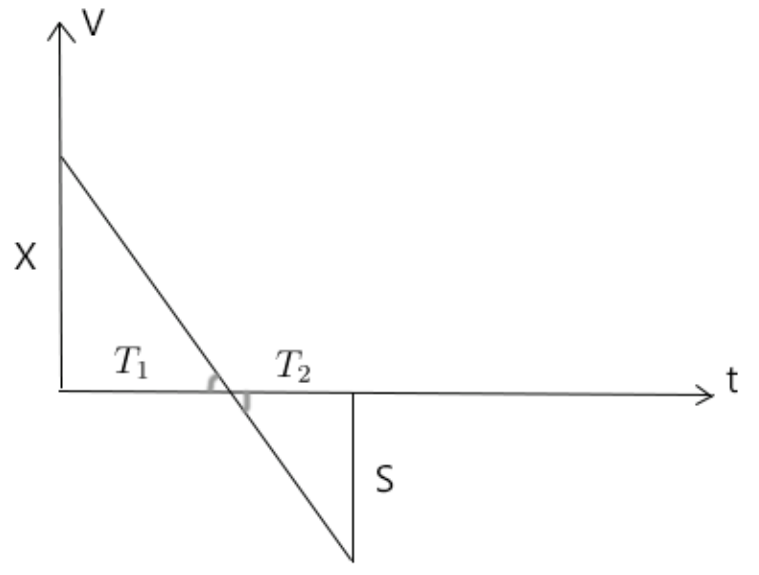
\includegraphics[scale=0.37]{images/1.png}

  Рис. 1: График модели управления запасами с задолженным дефицитом
\end{center}

Все предыдущие обозначения сохраняются с предущего параграфа с добавлением величины штрафа, а именно:
\begin{itemize}
	\item $\alpha$ - темп (объем спроса);
	\item $a$ - постоянные затраты поставки;
	\item $b$ - коэффицент затрат по хранению;
	\item $Q = \alpha \cdot T_1$ - величина поставки, размер партии;
	\item $L$ - величина суммарных затрат
	\item $g$ - величина штрафа за отсутствие запаса
	\item $X$ - максимальный объем запаса на складе
	\item $S$ - максимальный объем задолженного дефицита
\end{itemize}

В данной модели дефицит - это допущение отложенного спроса. В течение промежутка времени $T_1$ спрос удовлетворяется за счет имеющегося запаса. В течение $T_2$ запас отсутствует, возникает ситуация дефицита, постепенно накапливается долг величины $S$ по неудовлетворенному спросу. Этот долг удовлетворяется за счет поступившей партии $Q$, после чего на складе остается запас $X$ и все возобновляется по циклу. Длина цикла: $T=T_1 + T_2$.

Штраф за дефицит исчисляется на основе $g$ - издержек за единицу объёма дефицита за единицу времени.

Выразим данные величины через темп рост $\alpha$, как это делалось ранее:
$$X = \alpha T_1 \qquad S = \alpha T_2 \qquad Q = \alpha T$$

Величина суммарных средних затрат за цикл, которую по критерию оптимальности необходимо минимизировать, в данном случае выражается следующим образом:
$$L_{sr} = \frac{a+\frac{1}{2}bT_1X + \frac{1}{2}g T_2 S }{T_1 + T_2} \to \min$$
$$L_{sr} = \frac{a+\frac{1}{2}bT_1^2\alpha  + \frac{1}{2}g T_2^2 \alpha }{T_1 + T_2} \to \min$$
$$T_2 = \frac{b}{g} \cdot T_1 (?)$$

Приравниваем к нулю производные уравнений и решаем систему, получая оптимальные значения интервала удовлетворения спроса $T_1$ и интервала учета спроса (интервал отсутствия запаса и наличия дефицита) $T_2$:
$$T_1^* = \sqrt{\frac{2a}{b\alpha \cdot (1+\frac{b}{g})}}$$
$$ T_2^* = \frac{b}{g}  \sqrt{\frac{2a}{b\alpha \cdot (1+\frac{b}{g})}} =  \sqrt{\frac{2agb^2}{b\alpha \cdot (g+b) g^2}} =\sqrt{\frac{2ab}{\alpha \cdot (g+b) g}} $$

Если мы рссмотрим данные величины в пределе, то есть если коэффициент затрат по хранению будет меньше штрафа $g \to \infty$ (рост штрафа за дефицит приводит в пределе к запрету дефицита ввиду абсолютной невыгодности, $\frac{b}{g} \to 0$), то модель сведется к Формулам Уилсона, а дефицита и вовсе не будет в модели:
$$T_1^* \to \sqrt{\frac{2a}{b\alpha }} \qquad T_2^* \to 0$$

Найдем оптимальный маскимальный объем запаса на складе:
$$X^* = \alpha T_1 = \alpha  \sqrt{\frac{2a}{b\alpha \cdot (1+\frac{b}{g})}} $$

И оптимальный размер задолженного дефицита:
$$ S^* = \alpha T_2 = \alpha \sqrt{\frac{2ab}{\alpha \cdot (g+b) g}}$$

То есть при оптимальном случае, размер дефицита стремится к нулю $S^* \to 0$, а $X \to Q$.

\newpage
\subsection{Модель управления запасами с растянутой поставкой}

Рассмотрим модель с растянутой поставко и отсутствием дефицита. Пополнение запаса в такой модели происходит не мгновенно и занимает некоторое время, которым нельзя пренебречь и считать его равным $0$. График динамики запасов изображен ниже.

\begin{center}
  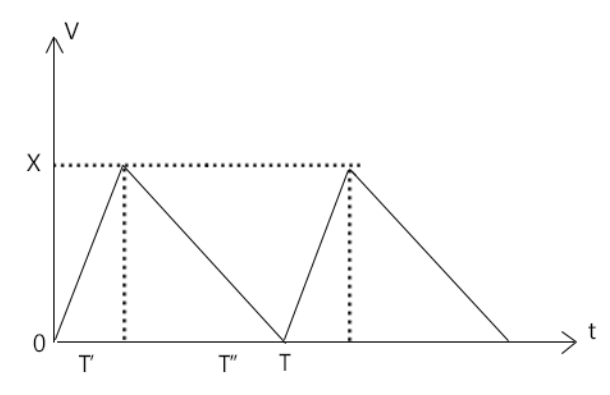
\includegraphics[scale=0.4]{images/2a.png}

  Рис. 2: График модели управления запасами с растянутыми поставками
\end{center}

На промежутке времени $T'$ продукция производится и отправляется на склад (но в то же время потребляется). Далее в течение промежутка $T''$ на оборудовании производится другая продукций, запас первой продукции не пополняется, он только потребляется. Через цикл управления запасами $T=T'+ T''$ на предприятии снова приступают к производству первой продукции и пополнению ее запасов. 

Постоянные затраты в такой ситуации связаны с переналадкой оборудования для запуска в производство партии изделий. Переменные затраты связаны с хранением.

Как известно, темп спроса $\alpha$.

\begin{definition}
	Обозначим за $\beta$ - \textbf{темп поставки} - объём поставки в единицу времени. 
\end{definition}

\begin{definition}
	\textbf{Реальная скорость пополнения} на промежутке $T'$ равна $\beta-\alpha$, эта разность определяет угол наклона прямой на промежутке $T'$: $\operatorname{tg} (\beta-\alpha)$. На промежутке $T''$ угол наклона прямой определяется величиной $\operatorname{tg} \alpha$.
\end{definition}

Все предыдущие обозначения сохраняются с предущего параграфа, а именно:
\begin{itemize}
	\item $\alpha$ - темп (объем спроса);
	\item $\beta$ - темп поставки
	\item $a$ - постоянные затраты поставки;
	\item $b$ - коэффицент затрат по хранению;
	\item $Q = \alpha \cdot T$ - величина поставки, размер партии;
	\item $L$ - величина суммарных затрат
	\item $T'$ - интервал поставки (время, в течение которого поступает партия)
	\item $T''$ - интервал отсутствия поставки
	\item $T$ - длина цикла управления запасами
	\item $X$ - максимальный объём запаса на складе
\end{itemize}

Выразим данные величины через темп рост $\alpha$, темп поставки $\beta$, как это делалось ранее:
$$X = \alpha T'' = (\beta-\alpha) \cdot T' \qquad Q = \alpha T \qquad $$
$$T = T' + T'' = \frac{X}{\beta-\alpha} + \frac{X}{\alpha}$$
$$Q = \alpha T = \alpha \cdot \left( \frac{X}{\beta-\alpha} + \frac{X}{\alpha}\right) = \frac{\alpha X}{\beta-\alpha} + X = \frac{X}{1-\frac{\alpha}{\beta}}$$
$$X =Q \cdot \left({1-\frac{\alpha}{\beta}}\right) = \alpha T \cdot \left({1-\frac{\alpha}{\beta}}\right)$$

Величина суммарных средних затрат за цикл, которую по критерию оптимальности необходимо минимизировать, в данном случае выражается следующим образом:
$$L_{sr} = \frac{a+\frac{1}{2}bXT}{T} = \frac{a+\frac{1}{2}b\alpha T^2 \cdot \left({1-\frac{\alpha}{\beta}}\right)}{T} = \frac{a}{T} + \frac{1}{2}b\alpha\left(1 - \frac{\alpha}{\beta} \right) \cdot T$$

Возьмем производную по $T$ и найдем оптимальный цикл поставки:
$$\frac{\partial L_{sr}}{\partial T} = - \frac{a}{T^2} + \frac{1}{2}b\alpha\left(1 - \frac{\alpha}{\beta} \right) = 0$$
$$T^2 = \frac{2a}{b\alpha\left(1-\frac{\alpha}{\beta}\right)}$$
$$T^* = \sqrt{ \frac{2a}{b\alpha\left(1-\frac{\alpha}{\beta}\right)}}$$

Если величина $\frac{\alpha}{\beta} \to 0$ в пределе, то формулы переходят в простейшую модель поставки, которая была рассмотрена ранее.

Из данного оптимального значения цикла поставки выведем другие оптимальные характеристики:
$$Q^* = \alpha \cdot T^* = \alpha \sqrt{ \frac{2a}{b\alpha\left(1-\frac{\alpha}{\beta}\right)}} = \sqrt{ \frac{2a\alpha}{b\left(1-\frac{\alpha}{\beta}\right)}}$$
$$X^* = Q^* \cdot \left({1-\frac{\alpha}{\beta}}\right) = \left({1-\frac{\alpha}{\beta}}\right) \sqrt{ \frac{2a\alpha}{b\left(1-\frac{\alpha}{\beta}\right)}}  =\sqrt{ \frac{2a\alpha\left(1-\frac{\alpha}{\beta}\right)}{b}} $$
$$L^* = a+\frac{1}{2}bX^*T^* = a +\frac{1}{2}b \sqrt{ \frac{2a\alpha\left(1-\frac{\alpha}{\beta}\right)}{b}} \cdot  \sqrt{ \frac{2a}{b\alpha\left(1-\frac{\alpha}{\beta}\right)}} = a + \sqrt{a \alpha}$$ 
$$T^{'*} = \frac{X^*}{\beta-\alpha} = \frac{\sqrt{ \frac{2a\alpha\left(1-\frac{\alpha}{\beta}\right)}{b}} }{\beta-\alpha} = \sqrt{\frac{2a\alpha}{\beta b (\beta-\alpha)}}$$
$$T^{''*} = \frac{X^*}{\alpha} = \frac{\sqrt{ \frac{2a\alpha\left(1-\frac{\alpha}{\beta}\right)}{b}} }{\alpha} = \sqrt{ \frac{2a\left(1-\frac{\alpha}{\beta}\right)}{\alpha b}} $$

\newpage
\subsection{Модель управления запасами с растянутой поставкой и задолженным дефицитом}

Рассмотрим модель с растянутой поставкой и допущением задолженного дефицита. 

Цикл управления разделяется на $4$ части:
$$T = T_1' + T_1'' + T_2' + T_2''$$

\begin{center}
  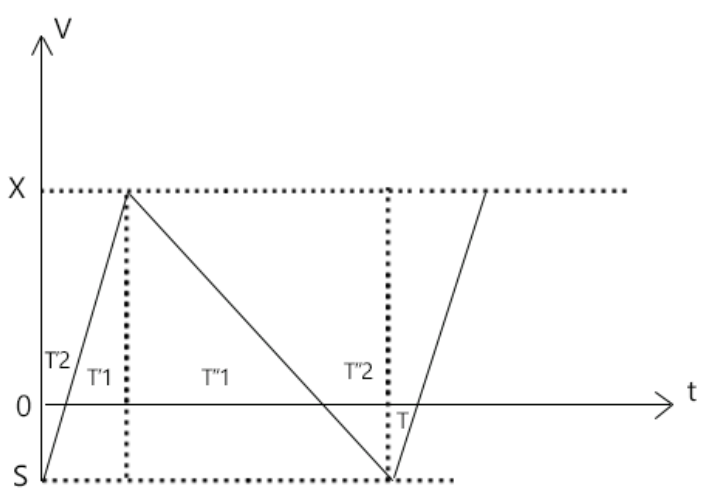
\includegraphics[scale=0.4]{images/3a.png}

  Рис. 3: График модели управления запасами с растянутой поставкой и задолженным дефицитомх
\end{center}

Как и в предущей модели в тот момент, когда приходит доставка запас увеличивается по какой-то линейной функции. Если $\beta$ - темп поставки, а $\alpha$ - темп роста, то угол наклона прямой разгрузки и поставки равен $\operatorname{tg} (\beta-\alpha)$.

В данной модели с дефицитом запасы уходят в минус со с тем же коэффициентом наклона прямой $\alpha$ и со скростью $\beta-\alpha$ повышаются.

Все предыдущие обозначения сохраняются с предущего параграфа, а именно:
\begin{itemize}
	\item $\alpha$ - темп (объем спроса);
	\item $\beta$ - темп поставки
	\item $g$ - величина затрат за единицу дефицита (величина штраф за отсутствие запаса)
	\item $a$ - постоянные затраты поставки, не зависят от объёма
	\item $b$ - коэффицент затрат по хранению;
	\item $Q = \alpha \cdot T$ - величина поставки, размер партии;
	\item $L$ - величина суммарных затрат
	\item $T_1'$ - интервал поставки (время, в течение которого поступает партия) (интервал наличия запаса и отсутствия дефицита)
	\item $T_1''$ - интервал удовлетворения спроса (интервал наличия запаса и отсутствия дефицита) в условиях отсутствия поставки
	\item $T_2'$ - интервал учета спроса (наличия дефицита и отсутствия поставки) в условияъ осуществления поставки
	\item $T_2''$ - интервал учета спроса (наличие дефицита и отсутствие запаса) в услових отсутствия поставки
	\item $T$ - длина цикла управления запасами
	\item $X$ - максимальный объём запаса на складе
	\item $S$ - максимальный размер дефицита
\end{itemize}

Рассмотрим разичные взаимосвязи между характеристиками, чтобы в последствии вычислить оптимальные характеристики:
$$X = \alpha T_1'' = (\beta-\alpha) \cdot T_1'$$
$$ S = \alpha T_2'' = (\beta-\alpha) \cdot T_2'$$
$$T = T_1' + T_1'' + T_2' + T_2'' = \frac{X}{\beta-\alpha} + \frac{X}{\alpha} + \frac{S}{\beta-\alpha} + \frac{S}{\alpha} = \frac{X+S}{\alpha \left(1-\frac{\alpha}{\beta}\right)}$$
$$Q = \alpha \cdot T = \alpha \frac{X+S}{\alpha \left(1-\frac{\alpha}{\beta}\right)} = \frac{X+S}{\left(1-\frac{\alpha}{\beta}\right)}$$
$$T_1 =T_1' + T_1'' \qquad T_2 = T_2' + T_2''$$

Величина суммарных средних затрат за цикл, которую по критерию оптимальности необходимо минимизировать, в данном случае выражается следующим образом:
$$L = \frac{a+\frac{1}{2}bT_1X +\frac{1}{2} g T_2 S}{T} = \frac{a+\frac{1}{2}bT_1X + \frac{1}{2}g T_2 S}{T_1 + T_2} \to \min$$

Должны минимизировать относительно $T_1,T_2,X,S$.
\begin{proof}
	Начнем вывод формул:
	$$T_1 = T_1'+T_1''  = \frac{X\beta}{\alpha(\beta-\alpha)} \Leftrightarrow X = \frac{\alpha(\beta-\alpha)}{\beta}T_1$$
	$$T_2 = T_2'+T_2'' = \frac{S\beta}{\alpha(\beta-\alpha)} \Leftrightarrow S = \frac{\alpha(\beta-\alpha)}{\beta}T_2$$

	Обозначим за
	$$\lambda = \frac{\alpha(\beta-\alpha)}{\beta} = \alpha \left(1 - \frac{\alpha}{\beta}\right)$$
	Подставим в формулу средних затрат вместо $X$ и $S$ выведенные значения:
	$$ L = \frac{a+\frac{1}{2}b\lambda T_1^2 + \frac{1}{2}g\lambda T_2^2 }{T_1 + T_2} \to \min $$

	Возьмем частные производные:

	$$ \frac{\partial L}{\partial T_1} = \frac{b\lambda T_1(T_1+T_2) - (a + \frac{1}{2}b\lambda T_1^2 + \frac{1}{2}g\lambda T_2^2)}{(T_1+T_2)^2} = 0$$
	$$ \frac{\partial L}{\partial T_1} = \frac{g\lambda T_2(T_1+T_2) - (a + \frac{1}{2}b\lambda T_1^2 + \frac{1}{2}g\lambda T_2^2)}{(T_1+T_2)^2} = 0$$

	Вычитая второе равенство из первого , получим следующее выражение:
	$$ (T_1+T_2) \lambda (bT_1 - gT_2) =0 \Rightarrow T_2 = \frac{b}{g}T_1$$

	Подставим $T_2$ в одно из равенств и решим относительно $T_1$ данное уравнение:
	$$ b\lambda T_1\left(T_1+\frac{b}{g}T_1\right) - \left(a + \frac{1}{2}b\lambda T_1^2 + \frac{1}{2}g\lambda \left(\frac{b}{g}T_1\right)^2\right) = 0$$
	$$ \frac{1}{2}b\lambda T_1^2 \left(1+\frac{b}{g}\right) = a$$

	Найдем оптимальные значения:
	$$T_1^* = \sqrt \frac{2a}{b\lambda (1+\frac{b}{g})} \qquad T_2^* = \frac{b}{g} \sqrt \frac{2a}{b\lambda (1+\frac{b}{g})} $$

	Через данные характеристики выводятся все остальные.

	Если $\frac{b}{g} \to \min , T_2^* = 0, S^* = 0$, то получится бездефицитная модель.
	Выразим $\lambda$: 
	$$ \lambda = \alpha (1-\frac{\beta}{\alpha})$$
	Если $\alpha \to 0$, то $\lambda \to \alpha $. И прямая становится все более вертикальной - разбираемся с растяжкой.
\end{proof}

\newpage
\subsection{Последовательность компьютерных моделей управления запасами}

\subsubsection{Модель 1. Определение оптимальной стратегии пополнения запасов в условиях полной определенности (период-неделя)}

Сначала мы строили простейшую модель, в которой в качестве исходных данных была информация за два периода времени и формат ввода исходных данных в данную и будущую неделю.

Расчетная форма состояла из двух частей - \textit{запасы, спрос, дефифит} в тоннах, а в правой части - \textit{данные о динамике денежных средств} - выручка, затраты, прибыль в рубля

\begin{center}
  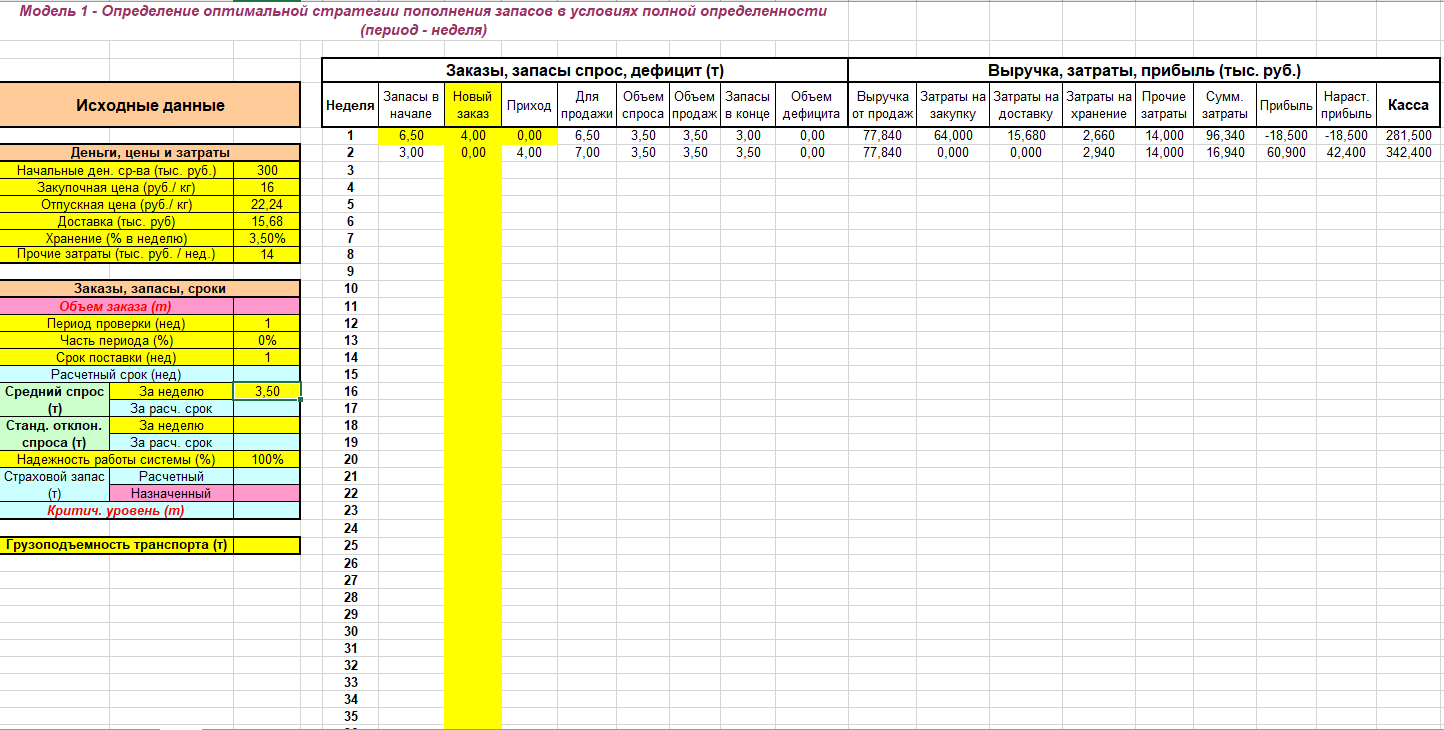
\includegraphics[scale=0.3]{images/4a.png}

  Модель 1
\end{center}

Мы вводили формулы и протягивали их вниз на $52$ недели, то есть на год. Необходимо было определить \textbf{размер поставки} (столбец Новый заказ) и \textbf{периодичиность поставки}. Для визулизации была построена диаграмма, отображаю динмику денежных средств и дефицита.

Поставки удовлетворялись двум условиям
\begin{enumerate}
	\item В системе не должно было быть дефицитов
	\item Поставки должны делать столбец Касса максимально возможным
\end{enumerate}

После этого мы по формулам Уилсона вывели оптимальные характеристиски управления запасами.

\subsubsection{Модель 2. Автоматическое определение критического уровня запасов}

Затем мы строили модель $2$ для автоматического определения уровня запасов, при достижении которого следовало подавать заказ на поставку. Для этого мы ввели несколько дополнительных столбцов (Заказы в пути, фиктивный запас), главным из которых являлся столбец \textsc{признак критического уровня}. Он показывал, когда фиктивный запас становился меньше фиксированного \textit{критического уровня} и являлся индикатором подачи заказа на поставку.

\begin{center}
  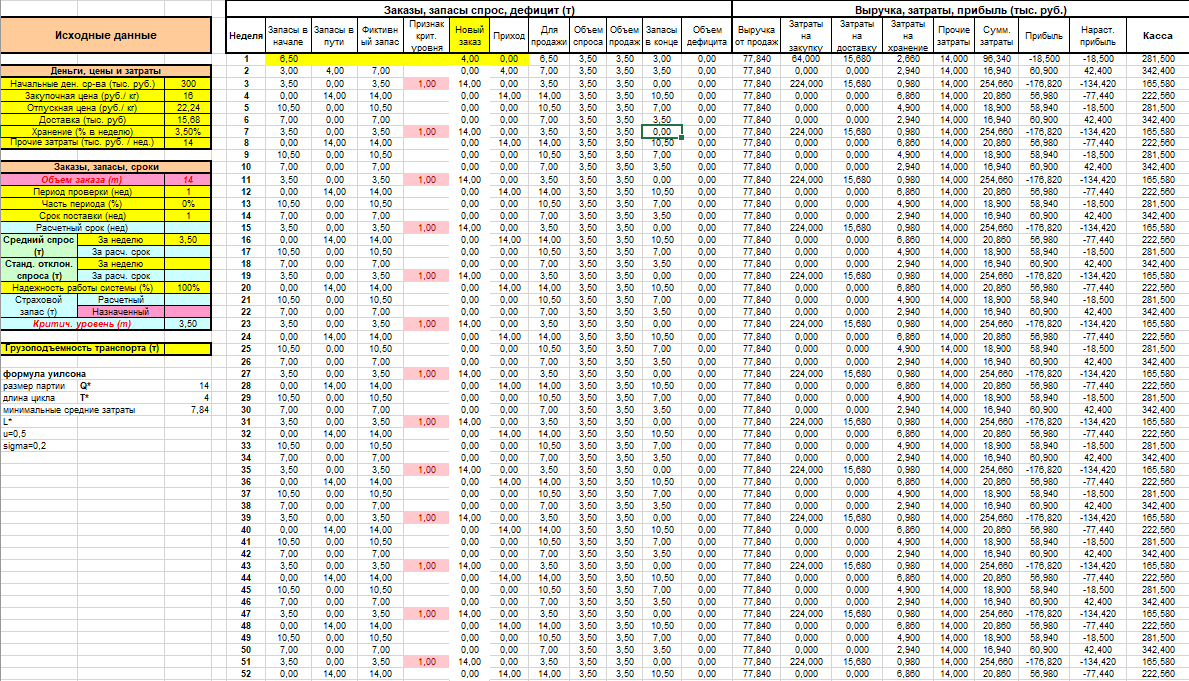
\includegraphics[scale=0.3]{images/4b.png}

  Модель 2
\end{center}

\subsubsection{Модель 3. Ежедневные данные}

Модель $3$ служила для обработки ежедневных данных в детерменированном случае.

\begin{center}
  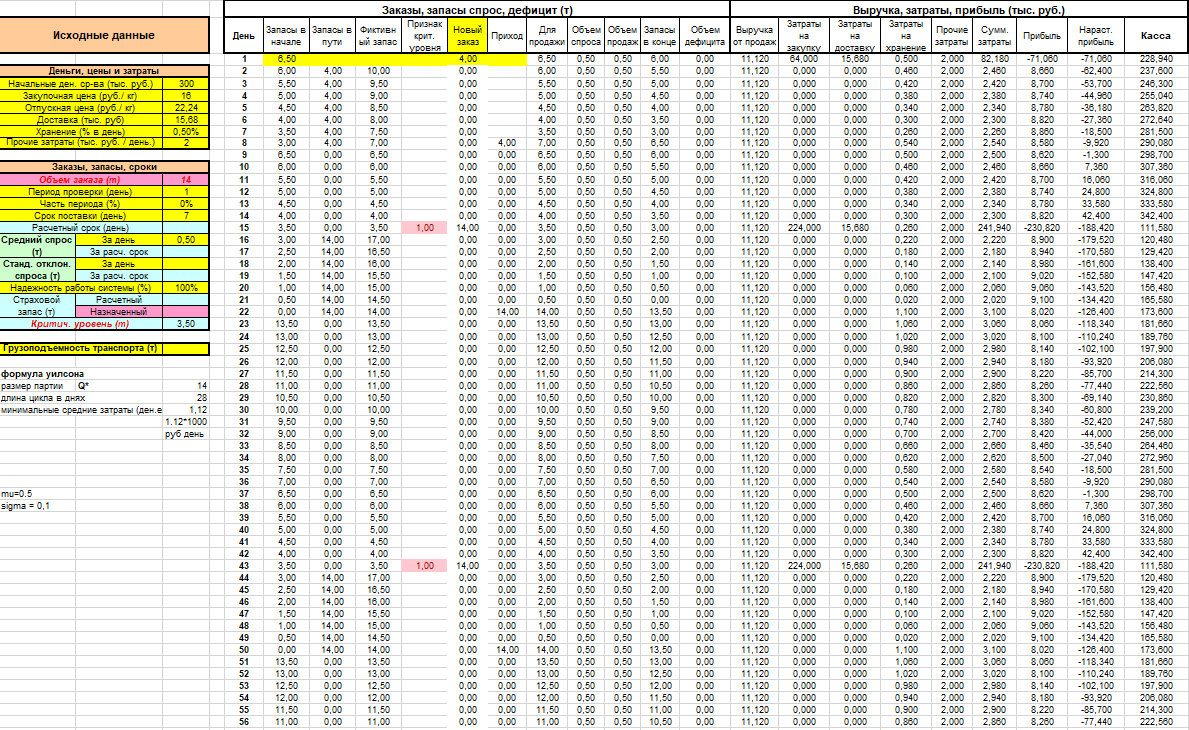
\includegraphics[scale=0.3]{images/4c.png}

  Модель 3
\end{center}

В исходных данных мы поделили на $7$ многие ячейки, чтобы преобразовать недельные данные в суточные, но срок проверки оставили равным $1$, так как проверка на наличие запасов должна происходить ежедневно. Так же был добавлен столбец \textsc{Приход}, в котором мы первый заказ сместили на $7$ дней вниз и данный столбец мы протянули вниз до конца года ($365$ дней). В результате получилась модель $3$.

\subsubsection{Модель 4. Организация обработки статистики в компьютерных моделях управления запасами}

Затем мы попытались смоделировать реальные системы управления запасов с помощью неопределенности в спросе. Мы хотели провести имитационное моделирование оптимальной стратегии управления запасами при заданном значении объема спроса и при неопределенности спроса. Для этого мы создали новый столбец \textsc{Сл.числ спрос} в модели $3$ и туда была введена формула \textsc{СЛЧИС} для случайной генерации спроса.

\begin{center}
  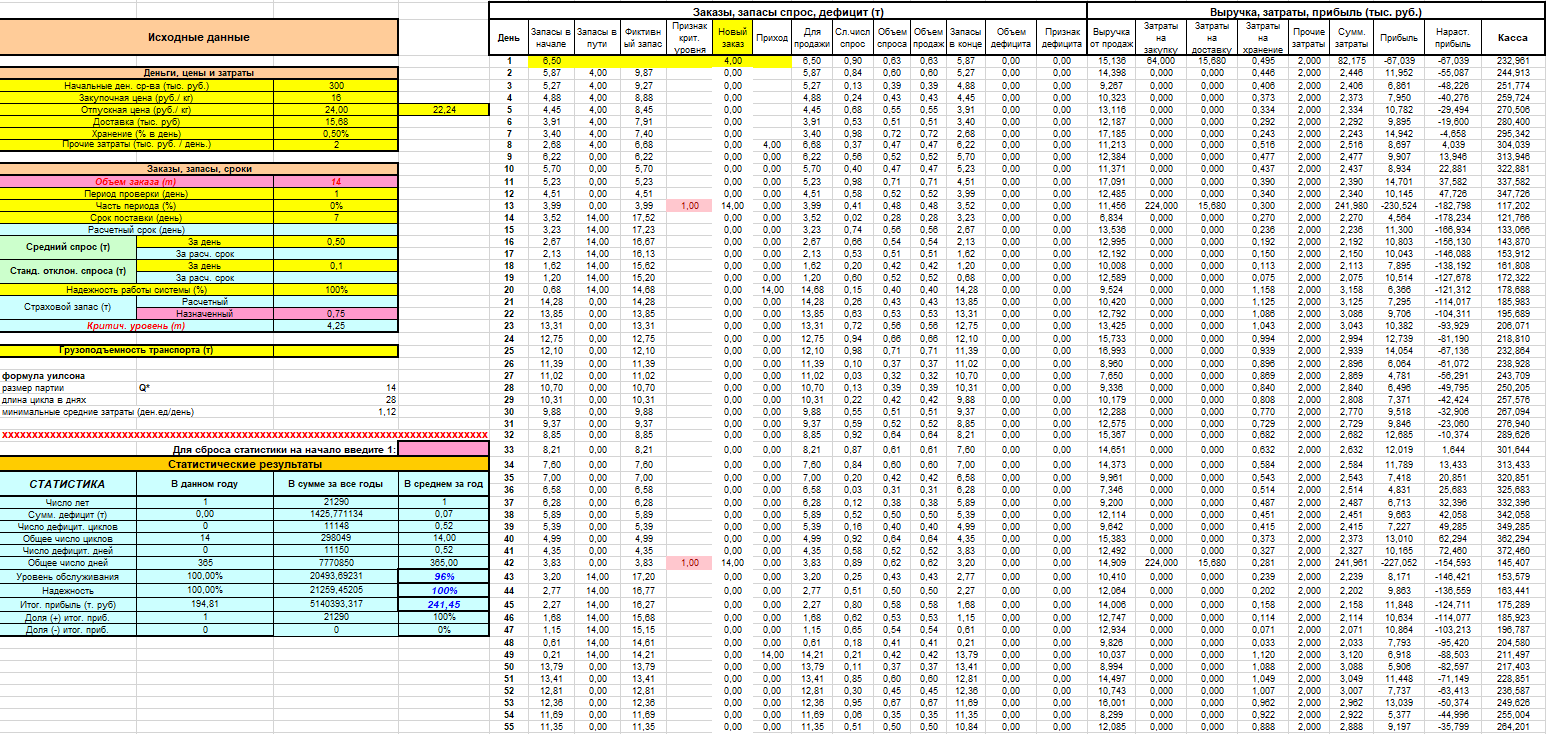
\includegraphics[scale=0.25]{images/4e.png}

  Модель 4
\end{center}

Из-за того, что при каждом пересчете числа случайные для спроса разные, то может возникать дефицит. В этом случае мы ввели понятие \textbf{страхового запаса} с заданным уровнем качества.

Величину страхового запаса мы хотели бы подобрать с помощью имитационного моделирования. Была построена следующая таблица имитацинного моделирования, содержащая $3$ столбца, с помощью которой мы хотели бы обрабатывать статистику.

\begin{center}
  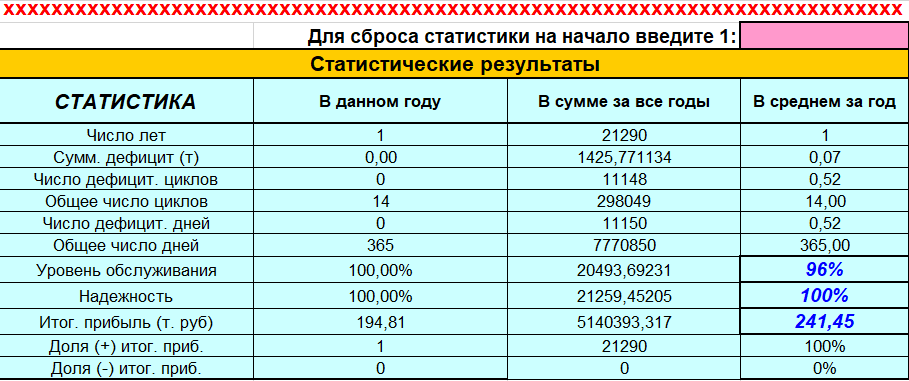
\includegraphics[scale=0.4]{images/4d.png}

  Обработка статистики
\end{center}

Очевидно, что первый столбец служит для расчета показателей по последнему году имитации, "в сумме за все годы" - накапливаются результыт по всем годам имитации, а "в среднем за год" данные в сумме за все года усредняются, делив на количество лет. Каждое нажатие обновления документа приводило к пересчету.

Некоторые полезные показатели выделены синим цветом:
\begin{itemize}
	\item \textsc{Уровень обслуживания} - числа дефицитных циклов должно быть как можно меньше, чтобы величина была ближе к $100$ процентам:
	$$\frac{\text{отношение общего числа циклов} - \text{число дефицитных циклов}}{\text{отношение общего числа циклов}}$$
	\item \textsc{Надежность} - число дефицитных дней должно быть очень небольшим, что величина надежности стремилась к $100$ процентам
	$$\frac{\text{общее число дней} - \text{число дефицитных дней}}{\text{общее число дней}}$$
	\item \textsc{Прибыль} - должна быть положительной при имитационном моделировании
\end{itemize}

\newpage
\subsubsection{Определение величины страхового запаса в компьютерных моделях управления запасами}

Имитацаионное моделирование мы проводили до тех пор, пока результаты при очередном обновлении не становились стабильными. Мы проводили имитационное моделирование на определение объема страхового запаса.

Ячейка критический уровень (\textsc{C27}) была равна величине среднего спроса, умноженного на срок поставки с прибавлением назначенного страхового запаса.

Для определения оптимального запаса необходимо было при заданном среднем спросе (ячейка \textsc{С20}) и при заданном уровне надежности системы (ячейка \textsc{C24}) подобрать такую величину страхового запаса, чтобы надежность была соответствующей, а уровень обслуживания варьировался в выбранной нами диапазоне доверия  (обычно выбирают больше $95\%$).

После этого строилась модель $5$, в которой было реализовано вероятностное распределение срока поставк.

\newpage
\section{Теория массового обслуживания}

\subsection{Общая схема системы обслуживания}

\begin{definition}
	\textbf{Теория массового обслуживания} является основной проектирования и анализа систем \textit{систем массивого обслуживания (СМО)}
\end{definition}

В борьбу за клиента в современной экономике вкладываются огромные средства. Во-многих слуяах неудовлетворенность клиента вызывается неудачной организацией его обслуживания (долгое ожидание в очереди, отказ обслуживания). Использование теории массового обслуживания позволяет фирме избежать подобных неприятностей.

На вход в \textsc{СМО} поступает \textit{поток требований} на обслуживание. В качестве требований могут выступать клиенты, пациенты, поломки в оборудовании и.т.д.

Требования поступают обычно в нерегулярные, случайные моменты времени. Случайный характер носит и продолжительность обслуживания. Все это создает нерегулярности в работе обслуживающей системы, является причиной ее перегрузок или недогрузок, причной сбоев в работе.

\begin{definition}
	\textbf{Детерменированный поток} - поток, который подчиняется некоторому расписанию.
\end{definition}
\begin{definition}
	\textbf{Регулярный поток} - поток с постоянным интервалом между соседними элементами.
\end{definition}

В \textsc{СМО} можно выделить четыер основных звена:

\begin{itemize}
	\item входящий поток требований
	\item накопитель
	\item узлы обслуживания
	\item выходящий поток
\end{itemize}

\begin{definition}
	\textbf{Накопитель} - место, где поступившие требования ждут начала обслуживания, перед тем как попасть в очередь. С накопителем могут связаваться пространственные или временные ограничения. 

	Накопитель может быть \textit{ограниченным} или неограниченным. Требование может пробыть некоторое время в очереди, покинуть ее, не дождавшись обслуживания. А может уйти в другую очередь.
\end{definition}

\begin{definition}
	\textbf{Узлы обслуживания} - место, где обслуживаются требования. В системе может быть один узнл, а может быть несколько. Число узлов может быть переменным (машина такси на остановке может рассматриваться как отдельный узел).

	Узлы могут быть \textit{универсальными} (обслуживающие любое требования) и \textit{специализированными}.

	Будучи универсальными они могут отличаться значениями своих характеристик. Среди таких характеристик одной из наиболее существенных является \textit{интенсивность обслуживания} - среднее число требований, которое способен обслужить узел в единицу времени.

	Узлы могут работать \textit{параллельно}, \textit{последовательно} или \textit{смешанным} образом.
\end{definition}

Обычно в каждый момент времени \textit{узел} обслуживает не более одного требования, но бывают \textsc{СМО}, в которых узлы обычно обслуживают сразу группы требований: преподаватель в вузе или экскурсовод.

\begin{definition}
	\textbf{Замкнутная} \textsc{СМО} - обслуженные требования после некоторой случайной, неизвестной заранее задержки опять поступают на вход.

	Замкнутой структурой является, например, поликлиника.
\end{definition}

\begin{definition}
	\textbf{Выходящий поток требований} - те требования, которые прошли обслуживание в узлах. Сам процесс обслуживания - случайный процесс.
\end{definition}

Мы рассмотрим базовые структуры и для рассмотренных ниже СМО предположим, что входящий поток является пуассоновским, а длительность обслуживания распределена по экспоненциальному закону. Это предположение применяется для широкого класса систем обслуживания и позволяют применить к изучению систем теорию \textit{марковских процессов}.

Давайте ознакомися с СМО!

\newpage
\subsection{Три свойства потоков требования}

Изучение потока требований нацелено на получение важнейших его характеристик. Характеристики вероятностного потока, естественно, являются вероятностными. 

К ним относятся, например:

\begin{enumerate}
	\item вероятности поступления того или иного числа требований на заданном отрезке времени;
	\item среднее число требований, поступающих за данное время;
	\item вероятностное распределение длин временных интервалов между соседними требованиями и т.д. 
\end{enumerate}

Оказывается, первая из названных характеристик является \textbf{фундаментальной}: зная ее, можно \textit{определить остальные}. 

Мы введем для нее специальное обозначение: \textsc{характеристика потока требования на промежутке}.

\begin{definition}
	$$V_k(t_0,t) $$ -  \textbf{вероятность возникновения $k$-требований} из рассматриваемого потока на промежутке времени, начинающийся в $t_0$ и имеет длину $t$.
\end{definition}

\begin{definition}
	$$V_{\geq k} (t_0,t) \qquad V_{\leq k} (t_0,t)$$ -  \textbf{вероятность возникновения не менее (не более) $k$-требований} (хотя бы $k$) из рассматриваемого потока на промежутке времени, начинающийся в $t_0$ и имеет длину $t$.
\end{definition}

\begin{definition}
	$$V_0(t_0,t)$$
	- \textbf{вероятность отсутствия требований} на нашем отрезке времени.
\end{definition}
\begin{definition}
	Вероятность $V_k(t_0,0)$:
	$$V_k(t_0,0) = \lim\limits_{t \to 0} V_k(t_0,t) \eqno(1.1)$$
	есть вероятность поступления $k$ требований на отрезке времени, длина которого равна $0$, то есть поступления $k$ требований в точке $t_0$ на оси времени.
\end{definition}

А следующее понятие поможет нам для анализа свойств потока:

\begin{definition}
	$x = o(x)$ - \textit{бесконечно малая величина} более высокого порядка, чем $x$, если:
	$$\lim\limits_{x \to 0} \frac{o(x)}{x} = 0 \eqno(1.2)$$
\end{definition}

Рассмотрим $3$ основных свойства потока требований

\subsubsection{Стационарность потока требования}

\begin{definition}
	Поток называется \textbf{стационарным}, если его базовая характеристика $V_k(t_0,t) $ не зависит от $t_0$, то есть не зависит от положения отрезка на оси времени (для двух отрезков $[t_0,t_0+t]$ и $[t_0',t_0' +t]$) выполнено равенство:
	$$ V_k(t_0,t) = V_k(t_0',t) \eqno(1.3)$$
\end{definition}

Вероятности $V_k$, а потому и другие вероятностные характеристики стационарного потока, не зависят от положения начальной точки, как следствие, и всего отрезка на оси времени.

В связи с этим для \textit{стационарных потоков} вместо $V_k(t_0,t)$ будем писать просто $V_k(t)$.

На относительно коротких промежутках многие потоки можно считать стационарными. В связи с этим длинный промежуток времени иногда разбивают на участки стационарности и рассматривают поток на каждом участке отдельно.


\subsubsection{Ординарность потока требований}

\begin{definition}
	Поток называется \textbf{ординарным}, если требования возникают по одному, то есть какова бы ни была точка $t_0$:
	$$\lim\limits_{t \to 0} \frac{V_{\geq 2}(t_0,t)}{t} = 0 \eqno(1.4)$$
\end{definition}

Условие \textit{ординраности} означает, что вероятность наступления хотя бы двух требований на отрезке $[t_0,t_0+t]$ стремится к $0$ при $t \to 0$ и при этом существенно быстрее, чем сама длина отрезка $t$.

Так как отрезок при $t \to 0$ стягивается в точку $t_0$, то свойство ординарности означает, что ни в какой момент времени $t_0$ \textit{невозможно наступление двух или более требований}, то есть в ординарном потоке требования поступают \textit{по одному}.

Условию $(1.4)$ можно придать другую эквивалетную формулировку через бесконечную малую величину - величину, стремящуюся к нулю быстрее, чем $t$:
$$V_{\geq 2}(t_0,t)  =  o(t) \eqno (1.5)$$

Если поток является стационарным, то условие ординарности упрощается и приобретает вид:
$$\lim_{t \to 0}  \frac{V_{\geq 2} (t_0,t)}{t} = 0 \eqno(1.6)$$
$$ V_{\geq 2} (t) = o(t) \eqno (1.7)$$

\subsubsection{Свойство отсутствия последействия}

\begin{definition}
	Поток требований называется \textbf{потоком без последействия}, если условные вероятности поступлений $k$ требований на произвольном отрезке, вычисленные при предположениях о распределении моментов поступления требований до $t_0$, совпадают с безусловной вероятностью.
\end{definition}

\textit{Отсутствие последействия} означает \textbf{независимость вероятностных характеристик потока} на отрезке времени от истории потока до этого отрезка, то есть означает внутреннюю независимость потока.

У потока отсутствует последействие, если его вероятностные характеристики, связанные с разными промежутками времени являются независимыми.
\begin{theorem}
	Для потоков \textit{без последействия} верна формула:
	$$V_k(t_0,t+\tau) = \sum_{m=0}^{k} V_m(t_0,t) \cdot V_{k-m} (t_0+t,\tau)\quad \eqno (1.8)$$
\end{theorem}
\begin{proof}
	Возьмем на оси времени два промежутка $t \text{ и } \tau$. 

	Определим вероятноть того, что за время $t+\tau$ событие наступит ровно $k$ раз. Это может осуществиться $k+1$ различными способами, а именно:

	\begin{itemize}
		\item за промежуток времени длительности $t$ произойдет $k$ событий, а за время $(t+\tau)$ - ни одного. Вероятность данного события:
		$$V_0(t_0,t) \cdot V_k(t_0+t,\tau)$$
		\item за промежуток времени длительности $t$ произойдет $k-1$ событий, а за время $(t+\tau)$ - 1. Вероятность данного события:
		$$V_1(t_0,t) \cdot V_{k-1}(t_0+t,\tau)$$
		\item за промежуток времени длительности $t$ произойдет $k-2$ событий, а за время $(t+\tau)$ - 2 
		\item $\ldots$
		\item за промежуток времени длительности $0$ не наступит ни одного события, а за время $(t+\tau)$  - $k$ событий.
	\end{itemize}

	Так как данные события являются независимыми и условная вероятность равна обычной вероятности, то по формуле полной вероятности, где в качестве события $A$ выступает вероятность наступления $k$ событий, получим следующую формулу, совпадаюущую с той, что мы пытались доказать:
	$$V_k(t_0,t+\tau) = \sum_{m=0}^{k} V_m(t_0,t) \cdot V_{k-m} (t_0+t,\tau)\quad \blacksquare \eqno (1.8) $$
	$$\sum_{k=0}^{\infty} V_k(t_0,t) = 1$$
\end{proof}

\begin{definition}
	Если поток удовлетворяет всем трем свойствам, то такой поток является \textbf{Пуассоновским}.
\end{definition}

\textbf{Примеры потоков:}
\begin{enumerate}
	\item стационарный + ординарный + отсутствие последствий: падение капли из не до конца завинченного крана.
	\item стационарный + ординарный + последствия: проходящая баржа под разведенными мостами ночью
	\item стационарный + не ординарный + последствия: машины, въезжающих на Володарский мост 
	\item стационарный + не ординарный + отсутствие последствий: поток пассажиров входящих в метро
	\item не стационарный + ординарный + последствия: появление поезда из туннеля в метро
	\item не стационарный + ординарный + отсутствие последствий: выход из квартиры человека
	\item не стационарный + не ординарный + отсутствие последствий: поток уборки станций в одно и то же время.
	\item не стационарный + не ординарный + последствия: появление вагонов из туннеля в метро
\end{enumerate}

\newpage
\subsection{Параметр и интенсивность потока}

Введем две важные характеристики потоков: \textit{параметр} и \textit{интенсивность}

\begin{definition}
	\textbf{Параметром стационарного потока} называется предел (если он существует для рассматриваемого потока):
	$$\lim_{t \to 0}  \frac{1 - V_{0} (t)}{t} = \lim_{t \to 0}  \frac{V_{\geq 1} (t)}{t} = \lambda \eqno (2.1)$$
\end{definition}

Так же можно записать определение предела на языке бесконечно малых функций:
$$1 - V_0(t) = V_{\geq 1}(t) = \lambda t + o(t)$$

Параметр показывает скорость сходимости к $0$ вероятности поступления хотя бы одного требования на отрезке $t$ при стремлении к $0$ длины отрезка. Очевидно, что параметр не может быть отрицательным.

Если параметр конечен, то:
$$V_{\geq 1}(0) = 0 \qquad V_0(t) = 1-\lambda t - o(t) = 1$$
то есть вероятность наступления хоты бы одного требования в точке равна $0$, а вероятность отсутствия требований равна $1$.

\begin{definition}
	\textbf{Интенсивностью стационарного потока} называется среднее число требований, поступающих из потока за единицу времени. Интенсивность обозначается буквой $\mu > 0$:
	$$\mu \cdot t = E(t) = \sum\limits_{k=0}^{\infty}k \cdot V_k(t) = \sum\limits_{k=1}^{\infty}k \cdot V_k(t)$$
	 - математическое ожидание числа требований.
\end{definition}

Если поток не предполагается стационарным, то значение параметра может меняться во времени. 

\begin{definition}
	Значением параметра в момент $t_0$ \textbf{(мгновенным значением параметра)} называется предел:
	$$\lambda (t_0) = \lim_{t \to 0}  \frac{1 - V_{0} (t_0,t)}{t} = \lim_{t \to 0}  \frac{V_{\geq 1} (t_0,t)}{t} \eqno (2.6)$$
\end{definition}

Аналогично может менять свое значение и интенсивность.
\begin{definition}
	Значением интенсивности в момент $t_0$ \textbf{(мгновенной интенсивностью)} называется предел
	$$ \mu (t_0) = \lim_{t \to 0}  \frac{\mathbb{E}(t_0,t)}{t} \eqno (2.7)$$
	где математическое ожидание числа требования на промежутке времени $\mathbb{E}(t_0,t)$:
	$$\mathbb{E}(t_0,t) = \sum_{k=0}^{\infty} k \cdot V_k(t_0,t) =  \sum_{k=1}^{\infty} k \cdot V_k(t_0,t) \eqno (2.8)$$.
\end{definition}

В стационарном случае значение $\lambda(t_0), \mu(t_0)$ постоянны:
$$\lambda(t_0) = \lambda, \quad \mu(t_0) = \mu$$

\begin{theorem}
	Мгновенные параметры и интенсивность связаны следующим соотношением: 
	$$\mu(t_0) \geq \lambda(t_0) \eqno(2.9)$$
\end{theorem}
\begin{proof}
$$\mathbb{E}(t_0,t) = \sum_{k=0}^{\infty} k \cdot V_k(t_0,t) =  \sum_{k=1}^{\infty} k \cdot V_k(t_0,t) \geq \sum_{k=1}^{\infty} V_k(t_0,t) = V_{\geq 1}(t_0,t)$$
$$\mathbb{E}(t_0,t) \geq  V_{\geq 1}(t_0,t)\eqno (2.10)$$
$$\mu (t_0) = \lim_{t \to 0}  \frac{\mathbb{E}(t_0,t)}{t} \geq  \lim_{t \to 0}  \frac{V_{\geq 1} (t_0,t)}{t} = \lambda(t_0) \Rightarrow \mu (t_0) \geq \lambda(t_0) $$
\end{proof}

\textbf{Следствие}: 

Для стационарных потоков выполняется 
$$\mu \geq \lambda \eqno(2.11)$$

\begin{proof}
	$$ \mu =\lim_{t \to 0} \frac{\sum_{k=0}^{\infty} k \cdot V_k(t)}{t} =\lim_{t \to 0} \frac{ \sum_{k=1}^{\infty} k \cdot V_k(t)}{t} \geq \lim_{t \to 0} \frac{ \sum_{k=1}^{\infty} V_k(t)}{t} =\lim_{t \to 0} \frac{ V_{\geq 1}(t)}{t} = \lambda$$
	$$\mu \geq \lambda $$ 	
\end{proof}

У потоков, моделирующих реальные процессы поступления требований, параметр (то есть предел (2.1) или (2.6)) обычно существует; в дальнейшем мы будем изучать только такие потоки.

\begin{theorem}
	Стационарные потоки, у которых параметр равен $0$ или $+\infty$ не представляют интереса для практики.
\end{theorem}
\begin{proof}
	Зафиксируем отрезок времени длины $t$, разделим его на $n$ равных частей. Если за время $t$ появилось хотя бы одно требование из потока, то это произошло хотя бы на одном из отрезков $\frac{t}{n}$. Следовательно:
	$$V_{\geq 1}(t) \leq n \cdot V_{\geq 1}(\frac{t}{n}) = \frac{V_{\geq 1}(\frac{t}{n})}{\frac{t}{n}} \cdot t$$
	где правая часть стремится к $\lambda t$ при $n \to \infty$. Таким образом:
	$$V_{\geq 1}(t) \leq \lambda t$$

	И если $\lambda = 0$, то вероятность возникновения хотя бы $1$ требования равна нулю, то есть ни на каком отрезке нет требований, список пуст и не содержит требований. Если $\lambda = + \infty$, то так как $\mu \geq \lambda$, то $\mu = +\infty$, то на любом отрезке $t$ бесконечное число требований $\mu t = +\infty$, поток является бесконечно плотным. 
\end{proof}

Для рассматриваемых в дальнейшем потоков всегда будет выполняться:
$$0 < \lambda < + \infty$$

Исходя из этого, мы можем теперь дать другую формулировку ординарности стационарных потоков, эквивалентную (1.6). 
$$\lim_{t \to 0}  \frac{V_{\geq 2} (t)}{t} = 0 \eqno(1.6)$$

\begin{theorem}
	Поток является ординарным тогда и только тогда, когда:
	$$\lim_{t \to 0}  \frac{V_{\geq 2} (t)}{t} = 0 \sim \lim_{t \to 0} \frac{V_{\geq 2}(t)}{V_{1}(t)} = 0 \eqno (2.15)$$
	то есть, когда вероятность поступления на малом отрезке в точке двух или меньшего числа требования есть величина более выоского порядка малости, чем вероятность наступления одонго требования
\end{theorem}
\begin{proof}
	Верно, что $$V_1(t) = V_{\geq 1}(t) - V_{\geq 2}(t) \eqno (2.16)$$
	так как:
	$$V_{\geq 1}(t) - V_{\geq 2}(t) = \sum\limits_{k=1}^{\infty} V_k(t) - \sum\limits_{k=2}^{\infty} V_k(t) = V_1(t)$$

	Откуда получаем:
	$$ \lim_{t \to 0} \frac {V_1(t) }{t} =\lim_{t \to 0} \frac {V_{\geq 1}(t) }{t} - \lim_{t \to 0} \frac {V_{\geq 2}(t) }{t} = \lambda - \lim_{t \to 0} \frac {V_{\geq 2}(t) }{t} \eqno (2.17) $$

	Пусть поток ординарен, то есть выполнено (1.6). Тогда из (2.17) следует:
	$$ \lim_{t \to 0} \frac {V_1(t) }{t} = \lambda \eqno (2.18)$$

	$$\lim_{t \to 0} \frac{V_{\geq 2}(t)}{V_1(t)} = \lim_{t \to 0} \frac{V_{\geq 2}(t)}{t} \cdot \lim_{t \to 0} \frac{t}{V_1(t)} = 0 \eqno (2.19)$$

	Достаточность тоже доказывается. 
\end{proof}

\textbf{Утв:} для стационарных потоков с конечной интенсивностью из условия $\mu = \lambda$ следует условие ординарности.

\textbf{Утв:} 
поток называется ординарным тогда и только тогда, когда
$$\lim_{t \to 0} \frac{V_{\geq 2}(t)}{V_{1}(t)} = 0 \sim \lim_{t \to 0} \frac{V_{\geq 2}(t)}{V_{\geq 1}(t)} = 0 $$


\textbf{Утв:} 
$$\lim_{t \to 0} \frac{V_{\geq 2}(t)}{V_{1}(t)} = 0 \sim \lim_{t \to 0} \frac{V_{1}(t)}{V_{\geq 1}(t)} = 1 $$


\newpage
\subsection{Пуассоновский поток в дискретном времени. Вывод формулы V0(t) для пуассоновского потока}

\begin{definition}
	Если поток удовлетворяет свойствам ординарности, стационарности и отсутствием последействия, то такой поток является \textbf{Пуассоновским}.
\end{definition}

\textbf{Пуассоновский поток в дискретном времени}

Представим себе, что ось времени разбита на примыкающие друг к другу маленькие отрезки одной и той же длины $\delta$:
\begin{center}
  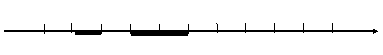
\includegraphics[scale=0.5]{images/4.png}

  Рис. 4: Пуассоновский поток
\end{center}

На каждом отрезке $\delta$ производится испытание, которое оканчивается удачей с вероятностью $p$ и неудачей с вероятностью $1-p$. Тогда последовательности отрезков, соответствующие удаче, можно рассматривать как \textit{последовательность требований}, поступающих из пуассоновского потока.

\begin{proof}
	Действительно:

	\begin{itemize}
		\item на каждом отрезке имеется лишь одно испытание - \textit{ординарность}
		\item вероятность удачи $p$ предполагается одной и той же, независимо от того, в аком месте на оси времени располоэен отрезок $\delta$ - \textit{стационарность}
		\item также вероятность удачи не зависит от того, чем кончились испытания на предыдущих отрезках - \textit{отсутствие последействия}.
	\end{itemize}
\end{proof}

Отличие пуассоновского потока состоит в том, что требования из потока поступают мгновенно, в то время как здесь этому соответствует целый отрезок длины $\delta$.

Данный поток называется \textit{пуассоновским потоком в дискретном времени}.

Чем меньше $\delta$, тем ближе наша последовательность зачерненных отрезков к последовательности требований, возникающих из пуассоновского потока. В пределе $\delta \to 0$ получаем пуассоновский поток.

Вероятность неудачи на $t$ отрезках подряд равна $q^t$. Аналогичная формула получится далее для пуассоновского потока.

\begin{definition}
	Пуассоновский поток в виду своей простоты называют иногда \textbf{простейшим}.
\end{definition}

Выведем формулу $V_0(t)$ для пуассоновского потока - \textbf{вероятности отсутствия требований} на промежутке времени длины $t$.
\begin{proof}

	Разделим единичный отрезок $n$ равных отрезков. Тогда:
	$$V_0(1) = \left(V_0\left(\frac{1}{n}\right)\right)^n \qquad V_0\left(\frac{1}{n}\right) = \left(V_0(1)\right)^{\frac{1}{n}}$$
	то есть вероятность отсутствия требований на единичном отрезке равно вероятности отсутствия требований на отрезке $\frac{1}{n}$ в $n$ степени.

	Рассматривая $k$ отрезок одинаковой длины $\frac{1}{n}$ получаем:
	$$V_0\left(\frac{k}{n}\right) = \left(V_0\left(\frac{1}{n}\right)\right)^k = \left(V_0(1)\right)^{\frac{k}{n}}$$

	То есть мы получили, что:
	$$V_0(t) = a^t \qquad t \in [0;1] \qquad V_0(1) = a$$
	откуда следует, что в виду монотонности вероятности, соотноение данное верно не только для рациональого, но и для любого $t\in[0,1]$.

	Любое число $t \in [0,+\infty]$ можно представить в виде суммы целой и дробной части. Формула верна и для любого $t \in [0,+\infty)$.

	Так как $a$-вероятность, то $0 \leq a \leq 1$. При $a=1$ - вероятность отсутствия требований равна $1$ и поток пуст. При $a=0$ - поток является бесконечно плотным, на любом отрезке наверняка есть требования. Оба эти случая не предоставляют интереса. Следовательно, $0 < a < 1$.

	Пусть $\alpha = - \ln \qquad 0 < \alpha < \infty$. Тогда:
	$$V_0(t) = a^t = e^{-\alpha t}$$

	Так как эспоненциальная функция может быть разложена через ряд Тейлора:
	$$e^x = 1 + \sum\limits_{n=1}^{\infty} \frac{x^n}{n!} = 1 + x + \frac{x^2}{2} + \ldots $$Параметр пуассоновского потока:
	$$\lambda  =\lim\limits_{t \to 0} \frac{1-V_0(t)}{t} = \lim\limits_{t \to 0}\frac{1-e^{-\alpha t}}{t} = \lim\limits_{t \to 0} \frac{1 - (1 - \alpha t + o(t))}{t} = \alpha$$

	Таким образом, $\lambda = \alpha$ и:
	$$V_0(t) = e^{-\lambda t}$$
\end{proof}

При выводе этой формулы мы не пользовались \textit{ординарностью потока}.

Очевидно, что чем большая время наблюдения, тем вероятность непоявления ни одного события меньше. Это соответствует тому, что если интенсивность появлений событий велика, то вероятность непоявления события быстро уменьшается со временем наблюдения.

Вероятность появления хотя бы одного события, наоборот, стремится со временем к единице, то есть при соответствующем длительном наблюдении событие таковое обязатеьно рано или поздно произойдет. Чем больше интенсивность появления события, тем быстрее наступает это событие и тем быстрее функция стремится к единице.

% 12 / 50

\newpage
\subsection{Вывод формул для вероятностей Vk элементарным методом}

Найдем вероятность поступления $k$ требований из пуассоновского потока на отрезке времени длины $t$.

Разделим отрезок $[0;t]$ на $n$ равных частей $n > k$.

Пусть $P_{k,n}'(t)$ - вероятность того, что на $[0,t]$ поступит $k$ требований, и при этом на каждой из $n$ частей окажется не более одного требования.

Пусть $P_{k,n}''(t)$ - вероятность того, что на $[0,t]$ поступит $k$ требований и при этом хотя бы на одной из $n$ частей окажется более одного требования. Тогда при любом $n$:
$$V_k(t) = P_{k,n}'(t) + P_{k,n}''(t)$$

Переходя в левой и правой части к пределу при $n \to \infty$, получим:
$$V_k(t) = \lim\limits_{n \to \infty} \left ( P_{k,n}'(t) + P_{k,n}''(t)\right)$$
$$P_{k,n}'(t) = C_n^k \cdot \left(V_1\left(\frac{t}{n}\right)\right)^k \cdot \left(V_0 \cdot \left(\frac{t}{n}\right)\right)^{n-k}$$
$$\left(V_0 \cdot \left(\frac{t}{n}\right)\right)^{n-k} = e^{-\lambda \cdot \frac{t}{n}(n-k)} = e^{-\lambda t} \cdot e^{\lambda t \frac{k}{n}}$$
$$\left(V_1\left(\frac{t}{n}\right)\right)^k = \left(1 - V_0\left(\frac{t}{n}\right) - V_{\geq 2} \left(\frac{t}{n}\right)\right)^k = \left(1 - e^{-\lambda \frac{t}{n}} + o\left(\frac{t}{n}\right)\right)^k=$$
$$=\left(1 - \left(1 - \lambda \cdot \frac{t}{n} + o\left(\frac{t}{n}\right)\right) + o\left(\frac{t}{n}\right)\right)^k = \left(\lambda \cdot \frac{t}{n} + o\left(\frac{t}{n}\right)\right)^k = $$
$$ = \frac{(\lambda t)^k}{n^k} \cdot \left(1 + \frac{o\left(\frac{t}{n}\right)}{\frac{t}{n}}\right)$$

Таким образом:
$$P_{k,n}'(t) = \frac{n!}{k! \cdot (n-k)!} \cdot  \frac{(\lambda t)^k}{n^k} \cdot \left(1 + \frac{o\left(\frac{t}{n}\right)}{\frac{t}{n}}\right) e^{-\lambda t} \cdot e^{\lambda t \frac{k}{n}}$$
но тут все пределы при $n \to \infty$ равны $1$.

Поэтому:
$$\lim\limits_{n \to \infty} P_{k,n}'(t) =  \frac{(\lambda t)^k}{k!}e^{-\lambda t}$$

А:
$$P_{k,n}''(t) \leq n \cdot V_{\geq 2}\left(\frac{t}{n}\right) = t \cdot \frac{ V_{\geq 2}\left(\frac{t}{n}\right)}{\frac{t}{n}}$$
и так как при $n \to \infty : \frac{t}{n} \to 0$, то имеем следующее по определению ординарности потока:
$$\lim\limits_{n \to \infty} P_{k,n}''(t) = 0$$

Поэтому формулы дают следующее выражение для вероятности возникновения $k$ требований в момент времени $t$:
$$V_k(t) = \frac{(\lambda t)^k}{k!}e^{-\lambda t}$$

Формула показывает, что для вычисления $V_k(t)$ нужно знать лишь одну вероятностную характеристику потока - значение его параметра $\lambda$. Пуассоновский поток полностью определяется значением его параметра. Два пуассоновских потока одинаковы, если равны их параметры.

Будет дан еще один метод вывод формулы - \textit{метод дифференциальных уравнений}.

\newpage
\subsection{Графики и свойства вероятностей Vk пуассоновского потока}

Рассмотрим, как выглядит графики вероятности $V_k$ (возникновения $k$ требований в момент времени $t$) для $\lambda = 0.25$ и $k = 0,\ldots, 15$.

\begin{center}
  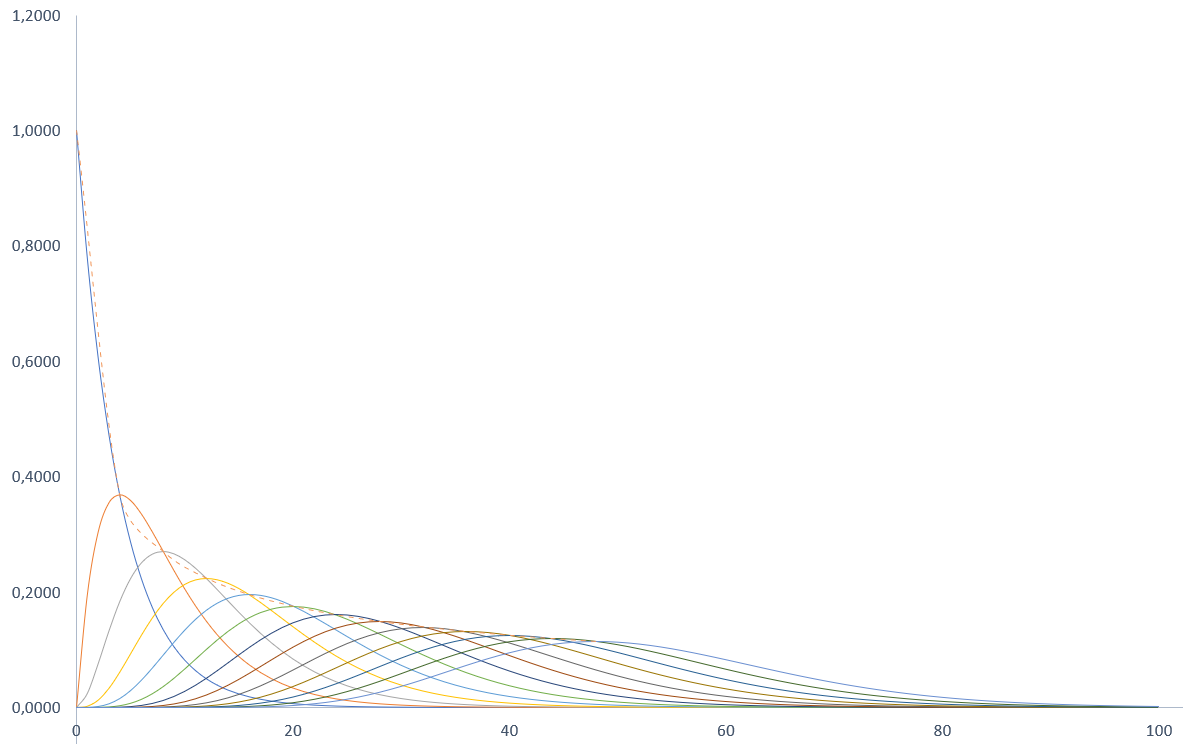
\includegraphics[scale=0.4]{images/6.png}

  Рис. 5: График вероятностей $V_k$ в зависимости от $t$ и $k$. $\lambda = 0.25$
\end{center}

На данных графиках мы можем видеть пунктирную линию. Эта линия соединяет точки максимумов каждого графика распределения вероятностей $V_k$. Можно видеть, что у каждой вероятност имеется единственная точка максимума и она находится на линии предыдущей вероятности, а еще эти максимумы равномено уменьшаются. Данный график позволил нам предсказать некоторые свойства вероятностей $V_k$ и давайте их докажем.

Реализация данного графика находится в файле:
$$\textsc{1. различные виды потоков.xlsx}$$

Вероятности $V_k(t)$ обладают следующими свойствами:

1. У каждой вероятности есть \textit{единственная точка максимума} и сама точка максимума находится на \textit{линии предыдущей вероятности}

\begin{proof}
	$$f(t) = \frac{(\lambda t)^k}{k!} \cdot e^{-\lambda t} \to \max $$
	$$\frac{\partial f(t)}{\partial t} = \frac{\lambda k (\lambda t)^{k-1}}{k!} \cdot e^{-\lambda t} - \lambda e^{-\lambda t} \frac{(\lambda t)^k}{k!} = 0$$
	$$e^{-\lambda t} \cdot \frac{(\lambda t)^{k-1}}{(k-1)!} = e^{-\lambda t} \frac{(\lambda t)^k}{k!} $$

	Действительно, точка максимума одна и в стационарной точке, являющейся максимумом, и совпадает с предыдущей вероятностью. 
\end{proof}


2. Точки максимумов располагаются \textit{равномерно} 
\begin{proof}
	Нам нужно доказать, что точки максимумов, являющиеся стационарными точками решений, убывают с одинаковым шагом.

	Возьмем выражение с предыдущего свойства для приравненной к нулю производной по $t$:
	$$e^{-\lambda t} \cdot \frac{(\lambda t)^{k-1}}{(k-1)!} = e^{-\lambda t} \frac{(\lambda t)^k}{k!} $$

	Заметим, что $\lambda \neq 0, k \geq 1, e^{-\lambda t} \neq 0$, то, следовательно, выражение принимает вид:
	$$\lambda t = k \Rightarrow t = \frac{k}{\lambda}$$

	Мы видим, что точки маскимума каждой вероятности $V_k$ находятся в момент времени $t$, причем он зависит от постоянного параметра $\lambda < 1$ и $k$, которая задает возрастающую последовательность. Следовательно, последовательность максимумов будет убывающей с шагом $t = \frac{k}{\lambda}$, то есть они располагаются равномерно, что и требовалось доказать
\end{proof}

3. Значение точек максимумов \textit{убывают с увеличением $t$}
\begin{proof}
	Подставим в исходную функцию значение точки максимума, выведенное в прошлом свойстве и воспользуемся Формулой Стирлинга: $k! \sim \sqrt{2\pi k} \left(\frac{k}{e}\right)^k$:
	$$f(\frac{k}{\lambda}) = \frac{k^k}{k!}e^{-k} = \frac{1}{k!}\cdot \left (\frac{k}{e} \right )^k \approx\frac{1}{\sqrt{2\pi k} \left(\frac{k}{e}\right)^k} \cdot \left (\frac{k}{e} \right )^k \sim \frac{1}{\sqrt {2\pi k}}$$

	Следовательно, последовательность точек максимумов стремится к нулю, что и требовалось доказать в данном свойстве.
\end{proof}

\subsubsection{Параметр и интенсивность пуассоновского потока}

Теперь докажем следующую теорему:
\begin{theorem}
	Интенсивность пуассоновского потока $\mu$ равна параметру $\lambda$.
\end{theorem}
\begin{proof}
	Так как 
	$$e^x = \sum\limits_{n=0}^{\infty} \frac{x^n}{n!}$$
	то можно записать следующую цепочку действий:
	$$\mu t = \mathbb{E}(t) =\sum_{k=0}^{\infty} k \cdot V_k(t) = \sum_{k=1}^{\infty} k \cdot V_k(t) (2.5) = \sum_{k=1}^{\infty} k \cdot \frac{(\lambda t)^k}{k!} \cdot e^{-\lambda t} =e^{-\lambda t}  \sum_{k=1}^{\infty} \frac{(\lambda t)^k}{(k-1)!} =$$
	$$=e^{-\lambda t} \lambda t \sum_{k=1}^{\infty} \frac{(\lambda t)^{k-1}}{(k-1)!} = e^{-\lambda t} \lambda t \sum_{k=0}^{\infty} \frac{(\lambda t)^{k}}{k!} =  e^{-\lambda t} \cdot \lambda t \cdot e^{\lambda t} = \lambda t$$
	Следовательно:
	$$\mu = \lambda$$
	
\end{proof}
\begin{theorem}
	В пуассоновском потоке дисперсия равна $D\xi = \lambda t$:
\end{theorem}
\begin{proof}
	$$E\xi^2 = \sum_{k=0}^{\infty} k^2 \cdot V_k(t) = \sum_{k=1}^{\infty} k^2 \cdot V_k(t) (2.5) = \sum_{k=1}^{\infty} k^2 \cdot \frac{(\lambda t)^k}{k!} \cdot e^{-\lambda t}=e^{-\lambda t}  \sum_{k=1}^{\infty} k \cdot \frac{(\lambda t)^k}{(k-1)!} =$$
	$$=e^{-\lambda t} (\lambda t)(\lambda t +1 ) e^{\lambda t} = \lambda t + \lambda^2 t^2$$
	$$ D \xi = E \xi^2 - (E \xi)^2 =\lambda t + \lambda^2 t^2 - (\lambda t)^2 =  \lambda t$$
\end{proof}

\newpage
\subsection{Распределение длин интервалов в пуассоновском потоке}

\textbf{Задача}

На шоссе мимо наблюдателя движется в одном направлении пуассоновский поток машин с известным значением параметра $\lambda$. В некоторый момент времени мимо наблюдателя проходит машина

\begin{enumerate}
	\item Найти вероятность того, что в течение заданного промежутка времени $t$ после этого момента мимо наблюдателя не прошла ни одна машина
	\item Пусть в течение времени $s$ после этого момента мимо наблюдателя не прошла ни одна машина. Найти вероятность того, что в течение заданного промежутка времени $t$, начинающегося в момент окончания $s$, мимо него не пройдет ни одна машина.
\end{enumerate}

\textbf{Решение:}

Пусть $\varphi_0(t)$ - условная вероятность отсутствия требований за время $t$ в первом пункте, а $\varphi(t |s )$ - во втором. Условие состоит в том, что этот промежуток времени начинает отсчитываться не с произвольного момента времени, а с такого, в который поступает требование. Ввиду отсутствия последействия:
$$\varphi_0(t) = V_0(t) = e^{-\lambda t}$$

Отсутствие последействия влечет независимость оставшегося времени ожидания $t$ от уже прошедшего $s$ - какое бы время наблюдатель ни провел в ожидании машины, предсказать отсутствие (или) появление машины на любом предстоящем отрезке времени он может с теми же шансами на успех, как если бы он совсем не ждал. 

Свойство отсутствия памяти - если время ожидания распределено о экспоненциальному закону, то информация о том, что событие не наступило к данному моменту не улучшает шансы на его поступление в дальнейшем.

Воспользуемся определением условной вероятности:
$$\varphi_0(\xi > t + s|\xi >t) = \frac{\varphi(\xi \geq t+s \cap \xi \geq t)}{\varphi_0(\xi \geq t)} = \frac{\varphi_0(\xi \geq t+s)}{\varphi_0(\xi \geq t)} = $$
$$ = \frac{1-(1-e^{-\lambda(t+s)})}{1-(1-e^{-\lambda t})} = \frac{e^{-\lambda(t+s)}}{e^{-\lambda t}} = e^{-\lambda s} = \varphi_0(\xi \geq s)$$

Мы получили совпадения условной и безусловной вероятности, следовательно $\varphi_0(t)$ есть экспоненциальная функция. Для стационарных и ординарных потоков отсутствие последействия эквивалентно \textit{экспоненциальности} функции $\varphi_0(t)$.

Действительно, вероятность $\varphi_0(t)$ тесно связана с функцией распределения $F(t)$ длин интервалов между соседними требованиями.

\begin{definition}
	Пусть $\xi$ - случайная величина - длина интервала между соседними требованиями в пуассоновском потоке.
\end{definition}

\begin{definition}
	\textbf{Функция распределения} $F_{\xi}(t)$ - функция, что ее значение в произвольной точке $t$ есть вероятность того, что длина интервала не превосходит $t$:
	$$F_{\xi}(t) = P(\xi \leq t)$$
\end{definition}

\begin{center}
  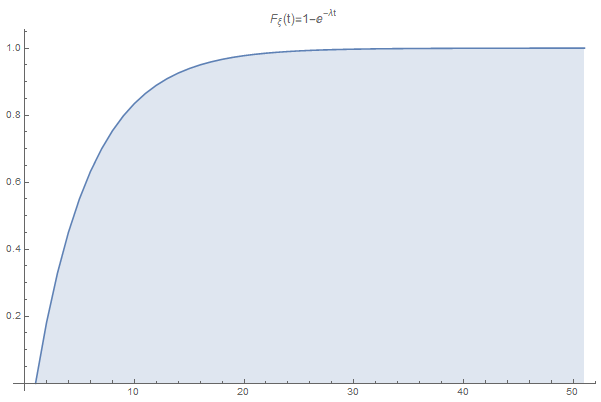
\includegraphics[scale=0.6]{images/7.png}

  Рис. 7: Функция экспоненциального распределения
\end{center}

Событие, состоящее в том, что $\xi \leq t$, совпадает с событием, состоящим в том, что за промежуток времени $t$, начинающийся в момент поступления требования $t$, поступит хотя бы одно требование:
$$V_{\geq 1}(t) = F_{\xi}(t) = P(\xi \leq t) = 1 -V_0(t) = 1-\varphi_0(t) = 1 - e^{-\lambda t}$$

\begin{definition}
	будем говорить, что случайная величина имеет абсолютное непрерывное распределение, если найдется функция $f_{\xi}(x) \geq 0$, что $\forall x \in \mathbb{R} (-\infty, \infty)$:
	$$F(x) = \int_{-\infty}^{x} f(t)dt$$
\end{definition}

$f_{\xi}(x)$ называется плотностью распределения случайной величины - функция, значение интеграла от нее на произвольном отрезке $[t_1,t_2]$ равно вероятности того, что $t_1 \leq \xi \leq t_2$

Если случайная величина $\xi$ имеет плотность распределения, то ее функция распределения непрерывна, поскольку интеграл - непрерывная функция верхнего предела.
$$ P(\omega : a \leq \xi(\omega) \leq b) =  F(b) - F(a) = \int_{-\infty}^b f(t)dt - \int_{-\infty}^a f(t)dt = \int_{a}^b f(t)dt$$

Свойства плотности вероятности:

\begin{enumerate}
	\item $\int_{-\infty}^{\infty} f(t)dt = 1$ - площад под кривой плотности распределения равна единице
	\item $f(x) = F'(x)$, если функция распределения дифференцируема
	\item $P(\xi = x ) = \int_{x}^{x} f(t)dt = 0$
\end{enumerate}

Пусть $[x;x+\delta x)$ - интервал произвольно малой длины. Вероятность попадания случайной величины в этот интервал приближенно равна проивезеднию значения плотности распределения в точке x на длину этого интервала. То есть пропорциональна длине интервала.

Выведем плотность распределения. $F_{\xi}(t)$ и $f_{\xi}(t)$ связаны с друг другом соотношением:
$$F_{\xi}(t) = \int\limits_0^t f_{\xi}(x)dx$$
$$f_{\xi}(t) = \frac{\partial F_{\xi (t)}}{dt} = \lambda \cdot e^{-\lambda t}$$

\begin{center}
  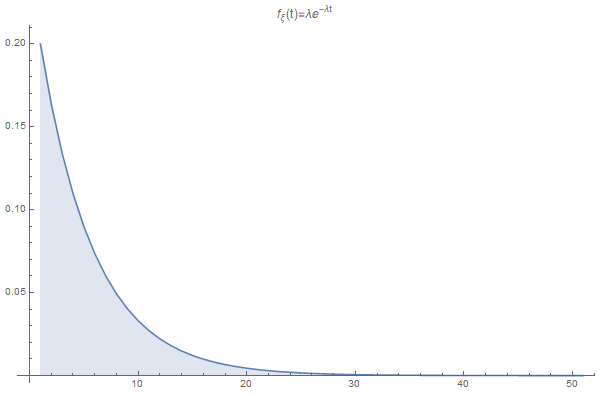
\includegraphics[scale=0.6]{images/8.png}

  Рис. 8: Плотность экспоненциального распределения
\end{center}

\begin{definition}
 	\textbf{Математическим ожиданием случайной величины $\xi$} с непрерывным распределением с плотностью распределения $f_{xi}(x)$ называется:
	$$ E\xi = \int\limits_{-\infty}^{\infty} x\cdot f_{\xi}(x)dx$$
	если данный интеграл абсолютно сходится, в противном случае говорят, что математическое ожидание не существует.
\end{definition} 

Найдем математическое ожидание интервала между соседними требованиями.

\begin{proof}
	Средняя длина интервала между соседними требованиями, то есть математическое ожидание $E\xi$ случайной величины $\xi$ определим по формуле:
	$$E\xi =  \int\limits_{0}^{\infty} x\cdot \lambda \cdot e^{-\lambda x}dx$$

	Проведем интегрирование по частям
	$$ \int_{0}^{\infty} udv = uv - \int_{0}^{\infty} vdu$$
	$$ u = \lambda x, du = \lambda dx, dv = e^{-\lambda x}, v = \frac{-e^{-\lambda x}}{\lambda}$$
	$$E\xi =  \int\limits_{0}^{\infty} x\cdot \lambda \cdot e^{-\lambda x}dx = \left(\lambda x \frac{-e^{-\lambda x}}{\lambda}\right)\left. \frac{}{}\right|_0^{\infty} - \int\limits_0^{\infty} \frac{-e^{-\lambda x}}{\lambda}\lambda dx = $$
	$$ = \left(-xe^{-\lambda x}\right)_0^{\infty} + \int\limits_0^{\infty} e^{-\lambda x} dx$$

	Заметим, что предел:
	$$\lim\limits_{x \to \infty} xe^{-\lambda x} = 0$$

	Тогда:
	$$E\xi = \int\limits_0^{\infty} e^{-\lambda x} dx = \frac{-e^{-\lambda x}}{\lambda} |_0^{\infty} = \frac{1}{\lambda}$$
\end{proof}

Мы определили среднюю длину промежутка между соседними требованиями в потоке. Она оказывается равной величине, обратной по значению параметру потока.

Мы получили, что вероятности $V_k(t)$ для пуассоновского потока простым способом выражаются через одну единственную $V_0(t)$. Вероятность $V_0(t)$ полностью определяется значением параметра $\lambda$, а значение $\lambda$ можно найти, зная вероятность $V_0(t)$ хотя бы для одного ненулевого конкректного значения $t=t_0$:
$$\lambda = - \frac{\ln V_0(t_0)}{t}$$

Таким образом, одно конкректное значение вероятности $V_0(t)$ полностью определяет все вероятностные характеристики пуассоновского потока.

\newpage
\subsection{Дисперсия длины интервала в пуассоновском потоке}

Дисперсия длины интервала в пуассоновском потоке равна:
$$D = \frac{1}{\lambda^2}$$

\begin{proof}
	$$D = \int\limits_{0}^{\infty} (x - \mathbb{E} )^2 \cdot f(x) dx =  \int\limits_{0}^{\infty} \left (x - \frac{1}{\lambda} \right)^2 \cdot \lambda e^{-\lambda x} dx$$
	$$E \xi^2 = \int\limits_{0}^{\infty} x^2 \cdot f(x) dx = \int\limits_{0}^{\infty} x^2 \lambda e^{-\lambda x} dx $$

	Проведем интегрирование по частям:
	$$ u = x^2, du = 2xdx, dv = \lambda e^{-\lambda x}, v = -e^{-\lambda x}$$
	$$ \int_{0}^{\infty} udv = uv - \int_{0}^{\infty} vdu$$
	$$\lim\limits_{\alpha \to \infty} \int_{0}^{\infty} x^2 \lambda e^{-\lambda x} dx = \lim\limits_{\alpha \to \infty} \left (x^2 \cdot (-e^{-\lambda x}) |^{\alpha}_{0} -  \int_{0}^{\alpha} 2x\cdot (-e^{-\lambda x}) dx \right ) = $$
	$$ = \lim\limits_{\alpha \to \infty} \left (x^2 \cdot (-e^{-\lambda x}) |^{\alpha}_{0} + 2 \cdot \frac{1}{\lambda} \int\limits_{0}^{\alpha} x \cdot \lambda\cdot (e^{-\lambda x}) dx \right )$$

	Видим, что второй предел в скобке является высчитанным на паром мат.ожиданием: $\mathbb{E} = \frac{1}{\lambda}$.
	$$E \xi^2 = \lim\limits_{\alpha \to \infty} \left (x^2 \cdot (-e^{-\lambda x}) |^{\alpha}_{0} + \frac{2}{\lambda^2} \right ) = 0 + \frac{2}{\lambda^2} = \frac{2}{\lambda^2}$$

	Следовательно, дисперсия равна:
	$$ D \xi = E \xi^2 - (E \xi)^2 = \frac{2}{\lambda^2} - \frac{1}{\lambda^2} = \frac{1}{\lambda^2}$$
\end{proof}

\newpage
\subsection{Случайная фильтрация пуассоновских потоков}

\begin{definition}
	\textbf{Случайная фильтрация (разрежение) потока} с вероятностью $p$ - операция, в результате применения которой каждое требование потока с вероятностью $p$ остается в нем, а с вероятностью $q=1-p$ удаляется из него. Эту операцию называют $p$-преобразованием.
\end{definition}

\begin{center}
  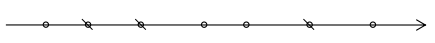
\includegraphics[scale=0.6]{images/9.png}

  Рис. 9: $p$-преобразование
\end{center}

\begin{theorem}
	Поток, получаемый в результате $p$-преобразования к пуассоновскому потоку, также является \textbf{пуассоновским}.
\end{theorem}
\begin{proof}
	Необходимо проверить, что полученный поток обладает тремя свойствами: стационарностью, ординарностью и отсутствием последействия.

	1) Вероятностные характеристики преобразованного потока зависят от $p$ и от характеристики исходного потока $\lambda$ параметра. Так как исходный поток стационарный, то и преобразованный тоже будет стационарным.

	2) Если за промежуток времени $t$ из преобразованного потока поступает не менее двух требований, то и из исходного так же поступает не менее двух. Следовательно, вероятности возникновения не мене $2$ требований равны:

	Структура потока не была изменена, следовательно, раз начальный поток был ординарным, то и преобразованный тоже явяется ординарным:
	$$V_{\geq 2}'(t) \leq V_{\geq 2}(t)$$ 

	3) Для проверки отсутствия последействия рассмотрим $V_0'(t)$. В преобразованном потоке требований нет за время $t$ в том и только том случае, когда их нет и в исходном поток, или и исходном потоке есть одно требование, но оно удалено, или в исходном потоке есть $2$ требования и они удалены. Таким образом:
	$$V_0'(t) = V_0(t) + V_1(t)q + V_2(t)q^2 + \ldots = \sum\limits_{k=0}^{\infty} V_k(t) \cdot q^k = $$
	$$ = \sum\limits_{k=0}^{\infty}\frac{(\lambda t)^k}{k!}\cdot e^{-\lambda t}\cdot q^k = e^{-\lambda t} \sum\limits_{k=0}^{\infty}\frac{(\lambda tq)^k}{k!} = e^{-\lambda t} \cdot e^{\lambda tq} = e^{-\lambda pt}$$

	Мы убедились в отсутствии последействия, а также получили параметр преобразованного потока:
	$$V_0'(t) = e^{-\lambda pt}$$
	$$\lambda' = \lambda p$$
\end{proof}

\textbf{Задача:}

По шоссе в одном направлении движется пуассоновский поток машин с интенсивностью $\mu = 2,5$ машины в минуту. Пост ГАИ,
находящийся на развилке, для разгрузки дальнейшей ремонтируемой части дороги, каждую машину с вероятностью $\frac{2}{3}$ отправляет в объезд по боковой дороге. Какова вероятность прохождения хотя бы одной машины в течение минуты мимо наблюдателя, стоящего на основной дороге? На боковой дороге?

\textbf{Решение:}

Вероятность удачи $p = \frac{1}{3}$, то есть машина поедет по ремонтной дороге и человек увидит ее в течение минуты хотя бы один раз:
$$V_{\geq 1}(t) = 1 - V_0(t) = 1- e^{-\lambda p t} = 1 - e^{-2.5\cdot \frac{2}{3} \cdot 1} \approx 0.56$$

Для наблюдателя, стоящего на второй дороге:
$$V_{\geq 1}(t) = 1 - V_0(t) = 1- e^{-\lambda p t} = 1 - e^{-2.5\cdot \frac{1}{3} \cdot 1} \approx 0.81$$


\newpage
\subsection{Объединение пуассоновских потоков}

Рассмотрим другой тип преобразования пуассоновских потоков. 

\begin{definition}
	\textbf{Объединение потоков} - операция объединения нескольких потоков в один поток.
\end{definition}
\begin{theorem}
	Если исходные потоки являются \textit{пуассоновскими} и \textit{независимыми} друг от друга, то их объединение тоже является \textbf{пуассоновским потоком}.
\end{theorem}
\begin{proof}
	Доказательство проведем для двух потоков, после чего методом математической индукции его можно распространить на любое количество потоков.

	Необходимо проверить, что полученный поток обладает тремя свойствами: стационарностью, ординарностью и отсутствием последействия.

	1) Характеристики объединенного потока зависят только от характеристик объединяемых потоков. Поскольку последние являются стационарными, то стационарным будет и результат их объединения.

	2) Для независимых потоков возможность одновременного поступления требования из одного потока и из другого практически нереализуема.

	Действительно, из объединенного потока за время $t$ поступает не менее $2$-х требований, то либо не менее двух поступает из одного из объединяемых потоков, либо из каждого поступает ровно по одному:
	$$V_{\geq 2}(t) \leq V_{\geq 2}'(t) + V_{\geq 2}''(t) + V_1'(t)\cdot V_1''(t)$$
	$$\frac{V_{\geq 2}(t)}{t} \leq \frac{V_{\geq 2}'(t)}{t} + \frac{V_{\geq 2}''(t)}{t} + \frac{V_1'(t)\cdot V_1''(t)}{t}$$Первые два слагаемых стремятся к нулю по определению ординарности, а:
	$$\frac{V_{\geq 2}(t)}{t} \leq e^{-t(\lambda' + \lambda'')}t \lambda'\lambda''$$
	в пределе $t \to 0$ дает бесконечно малую, таким образом, объединенный поток является ординарным ($V_1'(t) = o(\sqrt{t})$)

	3) Для доказательства отсутствия последействия заметим, что:
	$$V_0(t) = V_0'(t)\cdot V_0''(t) = e^{-t(\lambda' + \lambda'')}$$
	$$\lambda =  \lambda' + \lambda''$$

	Для другого доказательства отсутствия последействия, напишем формулу отсутствия последействия $(1.8)$, которую мы доказывали ранее по формуле полной вероятности:
	$$V_k(t) = \sum\limits_{n=0}^k V_n'(t) \cdot V_{k-n}''(t) = \sum\limits_{n=0}^k \frac{(\lambda't)^n}{n!}e^{-\lambda t} \cdot \frac{(\lambda'' t)^{k-n}}{(k-n)!}e^{-\lambda'' t} =$$
	$$ =  \frac{e^{-t(\lambda'+\lambda'')} \cdot t^k}{k!} \cdot \sum\limits_{n=0}^k \frac{k!}{n!(k-n)!}(\lambda')^n\cdot (\lambda'')^{k-n}$$

	Последняя формула является Биномом Ньютона, так как:
	$$(\lambda'+\lambda'')^k = \sum\limits_{n=0}^k \frac{k!}{n!(k-n)!}(\lambda')^n\cdot (\lambda'')^{k-n}$$
	так что:
	$$V_k(t) = \frac{e^{-t(\lambda'+\lambda'')} \cdot t^k}{k!} \cdot (\lambda'+\lambda'')^k = \frac{e^{-\lambda t}(\lambda t)^k}{k!}$$

	Следовательно, получили формулу вероятности для $k$ требований для пуассоновского потока по формуле отсутствия последействия. Объединенный поток обладает тремя свойствам, следовательно, он пуассоновский.
\end{proof}

\newpage

\subsection{Нестационарные потоки}

\begin{definition}
	\textbf{Простейшим потоком с возможной нестационарностью} называется поток, обладающий свойствами ординарности, отсутствия последействия, и имеющий в каждый момент времени $t$ конечное мгновенное значение параметра $\lambda(t)$.
\end{definition}

Очевидно, что пуассоновский поток является стационарным частным случаем потоков этого типа, для пуассоновского потока параметр является величиной постоянной:
$$\lambda(t) = \lambda$$

Простейшие потоки с возможной нестационарностью называют также \textit{нестационарными пуассоновскими потоками}.

\subsubsection{Вывод формул для V0(t0,t)}

Найдем вероятности $V_0(t_0,t)$ для потоков этого типа. Рассмотрим два примыкающих друг к другу отрезка времени $[t_0,t_0 + t]$ и $[t_0+t,t_0+t+\tau]$.

В силу отсутствия последействия по формуле $(1.8)$:
$$V_0(t_0,t+\tau) = V_0(t_0,t) \cdot V_0(t_0+t,\tau)$$

Так как $1-V_0(t) = V_{\geq 1}(t) = \lambda t + o(t)$, то:
$$V_0(t_0+t,\tau) = 1 - \lambda(t_0+t) \cdot \tau + o(\tau)$$

Тогда переходя к пределу при $\tau \to 0$ получаем:
$$V_0(t_0,t+\tau) = V_0(t_0,t) \cdot (1 - \lambda(t_0+t) \cdot \tau + o(\tau))$$
$$\frac{V_0(t_0,t+\tau)- V_0(t_0,t)}{\tau} = - \lambda(t_0+t)V_0(t_0,t) + \frac{o(\tau)}{\tau}$$
$$\frac{\partial V_0(t_0,t)}{\partial t} = -\lambda (t_0+t)V_0(t_0,t)$$
$$\frac{\partial \ln V_0(t_0,t)}{\partial t} = -\lambda (t_0+t)$$

Проинтегрируем обе части на отрезке $[0,t]$
$$\ln V_0(t_0,t) - \ln V_0(t_0,0) = -\int\limits_0^t \lambda(t_0+y)dy$$

Вероятность отсутствия требования равна $1$, следовательно:
$$V_0(t_0,0) = 1 \Rightarrow \ln V_0(t_0,0) = 0$$

Интеграл зависит от $t_0$ и $t$. Введем обозначения:
$$\Lambda (t_0,t) = \int\limits_0^t \lambda(t_0+y)dy$$

Произведем замену переменной:
$$\Lambda (t_0,t) = \int\limits_{t_0}^{t_0+t}\lambda(z)dz$$
$$\ln V_0(t_0,t) = -\int\limits_0^t \lambda(t_0+y)dy = - \Lambda (t_0,t)$$
$$V_0(t_0,t) = e^{- \Lambda (t_0,t)}$$

Так как пуассоновские потоки являются частным случае потока рассматриваемого типа, то формула должна оказаться обобщением соответствующей формулы $V_0(t) = e^{-\lambda t}$.

Чтобы убедиться в этом рассмотрим интегральное среднее функци $\lambda(z)$ на отрезке $[t_0,t_0+t]$:
$$\overline{\Lambda} (t_0,t) = \frac{1}{t}\int\limits_{t_0}^{t_0+t}\lambda(z)dz = \frac{1}{t}\Lambda(t_0,t)$$

Эта средняя величина равна высоте такого прямоугольника, построенного на основании $[t_0,t_0+t]$, площадь которого равна площади подграфика $\lambda(z)$ с тем же основанием ($\lim\limits_{t \to 0 } \overline{\Lambda}(t_0,t) = \lambda(t_0)$).

В частности, если функция $\lambda(z)$ является константой $\lambda(z) = \lambda$, то ее подграфик представляет прямоугольник и ее значение (высота прямоугольника) совпадает с интегральным средним. Таким образом, для потока с постоянным параметром:
$$V_0(t_0,t) = e^{- \overline{\Lambda} (t_0,t) t }  =  e^{-\lambda t}$$

Вероятность $V_0(t_0,t)$ не зависит от $t_0$ и ее обозначим за $V_0(t)$. Это то, что мы и хотели показать.

Вся нестационарность, имеющаяся в потоках рассматриваемого здесь типа, может быть выражена через нестационарность параметра. Если параметр постоянный, то и поток стационарный. Это обстоятельство позволяет для проверки на стационарность ограничиться проверкой неименности его параметра (или его интенсивности), как увидим даже.

\subsubsection{Вывод дифференциальных уравнений Vk(t0,t)}

Выведем формулы для вероятностей $V_k(t_0,t)$.
\begin{proof}
По формуле отсутствия последействия:
$$V_k(t_0,t+\tau) = \sum_{m=0}^{k} V_m(t_0,t) \cdot V_{k-m} (t_0+t,\tau)$$
$$V_k(t_0,t+\tau) = \sum_{m=0}^{k-2} V_m(t_0,t) \cdot V_{k-m} (t_0+t,\tau) + V_1(t_0+t,\tau) \cdot V_{k-1}(t_0,t) + V_0(t_0+t,\tau) \cdot V_k(t_0,t)$$

По условию ординарности $(1.5)$:
$$V_{\geq 2}(t_0+t,\tau) = o(\tau)$$

Так как $1-V_0(t) = V_{\geq 1}(t) = \lambda t + o(t)$, то:
$$V_0(t_0+t,\tau) = 1 - \lambda(t_0+t) \cdot \tau + o(\tau)$$
и
$$V_1(t_0+t,\tau) = 1 - V_0(t_0+t,\tau) - V_{\geq 2}(t_0+t,\tau) = \lambda(t_0+t) \cdot \tau + o(\tau)$$
то приведем к другому виду:
$$V_k(t_0,t+\tau) = o(\tau) + ( \lambda(t_0+t) \cdot \tau + o(\tau)) \cdot V_{k-1}(t_0,t) + (1 - \lambda(t_0+t) \cdot \tau + o(\tau)) \cdot V_k(t_0,t)$$
так как вероятность возникновения больше $2$ требований стремится к $0$ при $t \to 0$ и при этом существенно быстрее, чем сама длина отрезка $t$.

Преобразуем данное выражение привичным нам способом:
$$\frac{V_k(t_0,t+\tau) - V_k(t_0,t)}{\tau} = -\lambda(t_0+t) \cdot \left(V_k(t_0,t) - V_{k-1}(t_0,t)\right) + \frac{o(\tau)}{\tau}$$

При переходе к пределу при $\tau \to 0$:
$$\frac{\partial V_k(t_0,t)}{\partial t} = -\lambda(t_0+t) \cdot \left(V_k(t_0,t) - V_{k-1}(t_0,t)\right)$$

Это уравнение можно рассматривать как запись бесконечной системы уравнений, каждое из которых соответствует своему конкректному значению $k$ при $k \geq 2$, но по аналогичным рассуждениям оно верно и для $k \geq 0$, если положить $V_{-1}(t_0,t) \equiv 0$.

\subsubsection{Решение дифференциальных уравнений Vk(t0,t)}

Для решения системы введем производящую функцию:
$$f(t_0,t,x) = \sum\limits_{k=0}^{\infty} V_k(t_0,t) \cdot x^k$$

Умножим левую и правую часть на $x^k$ и просуммируем получившиеся равенства по всем $k$. Получаем:
$$\sum\limits_{k=0}^{\infty} \frac{\partial V_k(t_0,t)}{\partial t} x^k= -\lambda(t_0+t) \cdot \left(\sum\limits_{k=0}^{\infty} V_k(t_0,t)x^k - \sum\limits_{k=0}^{\infty} V_{k-1}(t_0,t)x^k\right)$$

Преобразуем в дифференциальное уравнение относительно функции $f$:
$$\frac{\partial f(t_0,t,x)}{\partial t} = -\lambda(t_0+t)(f(t_0,t,x) - x \cdot f(t_0,t,x))$$
$$\frac{\partial \ln f(t_0,t,x)}{\partial t} = -\lambda(t_0+t)(1-x)$$

Проинтегрируем обе части на отрезке $[0,t]$, получаем:
$$\ln f(t_0,t,x) - \ln f(t_0,0,x) = - \int\limits_0^t \lambda(t_0 + y)dy (1-x) = - \Lambda(t_0,t)(1-x)$$
$$f(t_0,t,x) = e^{-\Lambda(t_0,t)(1-x)} = e^{-\Lambda(t_0,t)} \cdot e^{\Lambda(t_0,t)x}$$

Разложим в ряд экспоненту:
$$e^{\Lambda(t_0,t)x} = \sum\limits_{k=0}^{\infty}\frac{(\Lambda(t_0,t)x)^k}{k!} = \sum\limits_{k=0}^{\infty}\frac{(\Lambda(t_0,t))^k}{k!} \cdot x^k$$

Подставим в формулу для производящей функции:
$$f(t_0,t,x) = \sum\limits_{k=0}^{\infty} V_k(t_0,t) \cdot x^k = e^{-\Lambda(t_0,t)}\sum\limits_{k=0}^{\infty}\frac{(\Lambda(t_0,t))^k}{k!} \cdot x^k$$
$$V_k(t_0,t) = \frac{(\Lambda(t_0,t))^k}{k!} \cdot e^{-\Lambda(t_0,t)}$$
где 
$$\Lambda (t_0,t) = \int\limits_0^t \lambda(t_0+y)dy = \int\limits_{t_0}^{t_0+t}\lambda(z)dz$$
	
\end{proof}

Приведенные рассуждения показывают, что данная формула является обобщенем формулы для пуассоновских потоков.

\subsubsection{Мгновенные параметр и интенсивность нестационарного потока, их связь}

\begin{theorem}
	Мгновенная интенсивность нестационарного простейшего потока $\mu(t_0)$ равна мгновенному значению параметра $\lambda(t_0)$:
	$$\mu(t_0) = \lambda(t_0)$$
\end{theorem}
\begin{proof}
	Проведем следующую цепочку преобразований:
	$$E(t_0,t) = \sum\limits_{k=0}^{\infty} k \cdot V_k(t_0,t ) = \sum\limits_{k=1}^{\infty} k \cdot V_k(t_0,t) =  \sum\limits_{k=1}^{\infty} k \cdot \frac{(\Lambda(t_0,t))^k}{k!} \cdot e^{-\Lambda(t_0,t)} = $$
	$$ = e^{-\Lambda(t_0,t)} \sum\limits_{k=1}^{\infty} \frac{(\Lambda(t_0,t))^k}{(k-1)!} = e^{-\Lambda(t_0,t)} \cdot \Lambda(t_0,t) \sum\limits_{k=0}^{\infty} \frac{(\Lambda(t_0,t))^k}{k!} = $$
	$$ = e^{-\Lambda(t_0,t)} \cdot \Lambda(t_0,t) \cdot e^{\Lambda(t_0,t)} = \Lambda(t_0,t)$$

	На основе доказанного предела:
	$$\mu(t_0) = \lim\limits_{t \to 0} \frac{E(t_0,t)}{t} = \lim\limits_{t \to 0} \frac{\Lambda(t_0,t)}{t} = \lambda(t_0)$$

	Тем самым равенство доказано. Оно является обобщением равенства $\mu = \lambda$ на случай простейшего потока с возможной нестационарностью.
\end{proof}

\newpage
\subsection{Неординарные потоки. Фомулы для Vk(t) для начальных k}

\begin{definition}
	\textbf{Простейший поток с возможной неординарностью} - поток, обладающий свойствами стационарности и отсутствия последействия. Требования могут поступать не по одному, а пакетами.
\end{definition}

Наряду с потоком требований следует рассматривать \textit{поток пакетов}, то есть новый поток, требования которого соответствуют пакетам требований исходного потока. В пакет объединяются все требования, поступающие одновременно.

Таким образом, несколько пакетов, поступивших одновременно, объединяются по определению в единый пакет, так что поток пакетов является ординарным.

Вероятность поступления $2$-х или большего числа пакетов за промежуток времени $t$ является величиной, бесконечно малой по отношению к $t$.

\begin{definition}
	Вероятность $V_0(t)$ - вероятность отсутствия пакетов, то есть вероятность отсутствия требований определяется так же , как и для пуассоновских потоков:
	$$V_0(t) = e^{-\lambda t} \eqno (10.1)$$
	так как при выводе этой формулы мы не пользовались ординарностью.

	Параметр потока требования равен параметру потока пакетов.
\end{definition}

Можно доказать, что при любом $k \geq 1$ существует предел:
$$\lim\limits_{t \to 0} \frac{V_k(t)}{V_{\geq 1}(t)} = p_k$$

Это выражение является условной вероятностью - вероятность возникновения $k$ требований за время $t$ при учете, что за это время $t$ поступает хотя бы одно требование. При $t \to 0$ отрезок $t$ стягивается в точку, так что в пределе мы получаем вероятность поступления $k$ требований в некоторый момент времени, если в него вообще поступают требования. Требования образуют пакет требований

Таким образом $p_k$ - вероятность того, что в поступившем пакете сожержится ровно $k$ требований.

Рассмотрим отрезок $\tau$ и примыкающий к нему $t$:
$$V_k(\tau + t) = \sum\limits_{m=0}^k V_m(\tau) \cdot V_{k-m}(t)$$
Так как $1-V_0(t) = V_{\geq 1} (t) = \lambda t + o(t) \Rightarrow V_0(t) = 1 - \lambda t + o(t)$, то при $k \geq 1$:
$$V_k(\tau + t) = V_0(\tau) \cdot V_k(t) + \sum\limits_{m=1}^k V_m(\tau) \cdot V_{k-m}(t) =  (1 - \lambda \tau + o(\tau))\cdot V_k(t) + \sum\limits_{m=1}^k V_m(\tau) \cdot V_{k-m}(t)$$
$$\frac{V_k(\tau + t) - V_k(t)}{\tau} = -\lambda V_k(t) + \sum\limits_{m=1}^k \frac{V_m(\tau)}{\tau} \cdot  V_{k-m}(t) + \frac{o(\tau)}{\tau}$$

Заметим, что по $(2.18)$:
$$\frac{V_m(\tau)}{\tau} = \frac{V_m(\tau)}{V_{\geq 1(\tau)}} \cdot \frac{V_{\geq 1(t)}}{\tau} \xrightarrow[t \to 0]{}p_m \cdot \alpha$$

Тогда мы получаем дифференциальное уравнение при $t \to 0$:
$$V_k'(t) = -\lambda \cdot V_k(t) + \lambda \cdot \sum\limits_{m=1}^k p_m \cdot V_{k-m}(t)$$

Это уравнение можно рассматривать как систему уравнений, каждое из которых соответствует своему значению $k$ для $k \geq 1$. Так как по $10.1$:
$$V_0(t) = e^{-\lambda t}$$ то
$$V_0'(t) = -\lambda e^{-\lambda t} = -\lambda V_0(t)$$

Если положить в дифференциальном полученном уравнении $k=0$, то оно будет выполнено, хоть и неосмысленно для суммы, поэтому будем считать, что оно выполнено $\forall k \geq 0$.

Приступим к решению данного дифференциального уравнения:
$$V_k'(t) = -\lambda \cdot V_k(t) + \lambda \cdot \sum\limits_{m=1}^k p_m \cdot V_{k-m}(t)$$
\begin{proof}
	Введем производящую функцию числа требований, поступающих за время $t$:
	$$q(t,x) = \sum\limits_{k=0}^{\infty} V_k(t) \cdot x^k$$
	и производящую функцию числа требований, содержащихся в пакете:
	$$h(x) = \sum\limits_{m=1}^{\infty}p_m \cdot x^m$$

	Умножим дифференциальное уравнение на $x^k$:
	$$V_k'(t) x^k= -\lambda \cdot V_k(t) x^k + x^k \lambda \cdot \sum\limits_{m=1}^k p_m \cdot V_{k-m}(t)$$
	просуммируем по $k=0,\ldots,\infty$ правые и левые части:
	$$\sum\limits_{k=0}^{\infty}V_k'(t) x^k = -\lambda \sum\limits_{k=0}^{\infty}V_k(t) x^k +  \lambda\sum\limits_{k=0}^{\infty} \left(x^k \cdot \sum\limits_{m=1}^k p_m \cdot V_{k-m}(t) \right)$$
	Рассмотрим коэффициент при $p_m$, получившийся в правой части после приведения подобных членов:
	$$\sum\limits_{k=0}^{\infty} \left(x^k \cdot \sum\limits_{m=1}^k p_m \cdot V_{k-m}(t) \right) = \sum\limits_{m=1}^{\infty} \left(p_m \cdot \sum\limits_{k=m}^{\infty} V_{k-m}(t) \cdot  x^k \right) =$$
	$$ = \sum\limits_{m=1}^{\infty} \left(p_m \cdot \sum\limits_{n=0}^{\infty} V_{n}(t) \cdot  x^{n+m} \right)= \sum\limits_{m=1}^{\infty} \left(p_m x^m \cdot \sum\limits_{n=0}^{\infty} V_{n}(t) \cdot  x^n \right) = q(t,x) \cdot h(x)$$

	Тогда перобразуем вышестоящее дифференциальное уравнение на языке производящих функций:
	$$\frac{\partial q(t,x)}{\partial t} = -  \lambda \cdot q(t,x) + \lambda \cdot q(t,x) \cdot h(x)$$

	Прологарифмировав получим:
	$$\frac{\partial \ln q(t,x)}{\partial t} =\lambda(h(x)-1) (?)$$
	Проинтегрируем обе части на отрезке $[0,t]$ и , так как вероятность поступления хотя бы одного требования в момент времени на отрезке времени длины $0$ равна $0$, то:
	$$\ln q(t,x) - \ln q(0,x) = \lambda \cdot (h(x)-1) \cdot t$$
	$$q(t,x) = e^{ \lambda \cdot (h(x)-1)} $$

	Мы нашли производящую функцию числа требований, поступающих за время $t$:
	$$q(t,x) = e^{ \lambda \cdot (h(x)-1)}  = e^{-\lambda t}e^{\lambda t \cdot h(x)} = e^{-\lambda t} \sum\limits_{n=0}^{\infty}\frac{(\lambda t h(x))^n}{n!} =\sum\limits_{n=0}^{\infty}\frac{(\lambda t)^n}{n!} \left( \sum\limits_{m=1}^{\infty}p_m \cdot x^m\right)^n$$

	Мы нашли производящую функцию, теперь найдем оставшийся коэффициет $x^k$, чтобы выразить все.

	Зафиксируем $k$ и найдем сначала коэффициент при $x^k$, который получается в выражении:
	$$\left( \sum\limits_{m=1}^{\infty}p_m \cdot x^m\right)^n$$
	после возведения в степень (умножения суммы на себя $n$ раз и приведения подобных членов). Обозначим этот коэффициент посредством $Q_k^{(n)}$.

	При $n=0$ выражение обращается в $1$, так что: 
	$$Q_k^{(0)}\begin{cases}
		1, k =0 \\
		0, k \geq 1
	\end{cases}$$

	При произвольном $n \geq 1$:
	$$Q_k^{(n)} = \begin{cases}
		0, k \leq n -1 \\
		\sum\limits_{\sum\limits_{j=1}^n m_j = k} \prod\limits_{j=1}^n p_{m_j}, k \geq n
	\end{cases}$$

	Данное равенство верно для любых $n, k \geq 0$. При фиксированном $k$ и растущем $n$ лишь конечное число коэффициентов отлично от нуля.

	Тогда вероятности $V_k(t)$ можно выразить через $Q_{k}^{(n)}$:
	$$V_k(t) = e^{-\lambda t}\sum\limits_{n=0}^{\infty}\frac{(\lambda t)^n}{n!} \cdot Q_{k}^{(n)} =  e^{-\lambda t}\sum\limits_{n=0}^{k}\frac{(\lambda t)^n}{n!} \cdot Q_{k}^{(n)}$$

	То есть общий вид формулы:
	$$V_k(t) = e^{-\lambda t}\sum\limits_{n=0}^{k} \left(\frac{(\lambda t)^n}{n!} \cdot \sum\limits_{\sum\limits_{j=1}^n m_j = k} \prod\limits_{j=1}^n p_{m_j}\right)$$

	Каждое слагаемое внешней суммы при том или ином значении $n$ соответствует поступлению определенного числа пакетов, каждое слагаемое само распадается в сумму (внутренняя сумма), слагаемые которой соответствуют возможным распределениям $k$ требований по пакетам.
\end{proof}

\textbf{Вывод:} вероятностные характеристики простейшего потока с возможной неординарностью полностью определяются значением параметра $\lambda$ и вероятностями $p_m$ того, что в пакете содержится $m$ требований. 

При $k=0$:
$$V_0(t) = e^{-\lambda t}$$

Слагаемые в формулах имеют естественную интерпретацию. Поступление одного требования за время $t$ возможно, когда за это время поступает один пакет и в нем сожержится $1$ требование. 

При $k=1$:
$$V_1(t) = e^{-\lambda t} \cdot \lambda t \cdot p_1$$

Поступление двух требований за время $t$ означает либо поступление одного пакета с двумя требованиями, либо двух пакетов с одним требованием в каждом. Первое слагаемое - вероятность поступления одного пакета на вероятность $p_2$, что в этом пакете содержится два требования,  второе - вероятность поступления двух пакетов на вероятность $p_1^2$ того, что в каждом из них содержится по одному требованию.

При $k=2$:
$$V_2(t) = e^{-\lambda t} \cdot \lambda t \cdot p_2 + e^{-\lambda t} \frac{(\lambda t)^2}{2!} \cdot p_1^2$$

\newpage
\subsection{ Параметр и интенсивность неординарного потока}

Найдем интенсивность $\overline{\mu}$ требований простейшего потока с возможной неординарностью. Обозначим посредством $c$ - среднее число требований в пакете:
$$c = \sum\limits_{i=1}^{\infty} m \cdot p_m \geq \sum\limits_{i=1}^{\infty}p_m  = 1$$

$\mu$ - интенсивность пуассоновского потока. 

\begin{theorem}
	Верно равенство $\overline{\mu} = c \cdot \mu$	
\end{theorem}
\begin{proof}
	Зафиксируем отрезок времени $t$. Если за время $t$ поступает $n$ пакетов, то среднее число требований составляет $cn$ ($E(c\xi) = c E\xi)$. Вероятность поступления $n$ пакетов равна:
	$$\frac{(\lambda t)^n}{n!} \cdot e^{-\lambda t}$$

	Следовательно, среднее число требований за время $t$ есть вероятность сумма вероятностей получения $n$ пакетов на среднее значение числа требований в $n$ пакетах, то есть:
	$$\overline{\mu} \cdot t =  \sum\limits_{n=1}^{\infty} c \cdot n \cdot \frac{(\lambda t)^n}{n!} \cdot e^{-\lambda t} = c \mu t$$
	$$\overline{\mu} = c \cdot \mu$$
\end{proof}

Равенство $\overline{\mu}= \lambda = \mu$ происходит при $c=1$, а такое возможно, если вероятность $1$ требования в пакете равна $1$, а все а вероятность другого любого числа требования равно $0$ ($p_1=1,p_m=0 \qquad m \geq 2$), то есть когда в каждом пакете содержится ровно одно требование и, тем самым, поток является ординарным и, следовательно, пуассоновским.

\textbf{Утверждение:} равенство интенсивности и параметра равносильно ординарности потока.

Мы распространим это утверждение на случай потоков с последействием. Если поток является неординарным, то его интенсивность строго больше параметра.  

\begin{theorem}
	Если $p_1=1,p_m=0 \qquad m \geq 2$ условие выполняется, то формулы для неординарного потока переходят в формулы для пуассоновского потока.
\end{theorem} 
\begin{proof}
	Действительно, при $n<k$ сумма, равная $k$, больше, чем число слагаемых $n$. Следовательно, хотя бы для одного $m_j$ выполняется неравенство $m_j \geq 2$, что обращает в $0$ каждое произведение $n<k$. 

	При $n=k$ сумма $\sum\limits_{j=1}^n m_j$ равна числу составляющих слагаемых. Это возможно, если $m_j=1$. Тогда внутренная сумма состоит из одного слагаемого, имеющего вид произведения, все сомножители которого равны $1$. Следовательно, вся внутренняя сумма равна $1$, а рассматриваемое слагаемое внешней суммы равно:
	$$\frac{(\lambda t)^k}{n!}=\frac{(\lambda t)^k}{k!}$$

	Таким образом, получается, что при условии $p_1=1,p_m=0 \qquad m \geq 2$ формула преобразуется в:
	$$V_k(t) = \frac{(\lambda t)^k}{k!} e^{-\lambda t}$$
	совпадающую с формулами вероятности пуассоновского потока, что и требовалось доказать.
\end{proof}

\newpage
\subsection{Потоки с последействием. Функции Пальма-Хинчина. Вывод системы дифференциальных уравнений для Vk(t0, t)}

\begin{definition}
	\textbf{Простеший поток с возможным последействием} - поток, обладающий свойствами стационарности и ординарности, но не обладающий третим свойством пуассоновского потока.

	Условная вероятность постулпления некоторого числа требований на $t$, вычисленная при предположениях о предыстории потока, может отличаться от безусловной вероятности.
\end{definition}

Рассмотрим промежуток времени $\tau$ и примыкающий к нему справа промежуток $t$. Пусть $h_k(\tau,t)$ - вероятность того, что за время $\tau$ поступит хотя бы одно требование и за $t$ поступит ровно $k$ требований. Тогда:
$$\frac{h_k(\tau,t)}{V_{\geq 1}(\tau)}$$
является улсовной вероятность - вероятность поступления $k$ требований на промежутке времени $t$  при условии, что на $\tau$ поступает хотя бы одно требование, действительно:
$$V_k(t | \tau) = \frac{h_k(\tau,t)}{V_{\geq 1}(\tau)}$$

Если бы события, связанные с промежутками $\tau$ и $t$ были независимыми, то эта дробь оказалась бы равна вероятности $V_k(t)$ по определению независимости. Но мы такой независимости не предполагаем.

\begin{definition}
	\textbf{Функция Пальма-Хинчина} - предел следующего выражения:
	$$\lim\limits_{\tau \to 0} \frac{h_k(\tau,t)}{V_{\geq 1}(\tau)} = \varphi_k(t)$$
	- вероятность поступления $k$ требований за время $t$ при условии, что в начальный момент этого промежутка $t$ поступает хотя бы одно (по ординарности одно) требовани.
\end{definition}

Рассмотрим событие, состоящее в том, что за время $\tau+t$ поступает $k$ требований. Обозначим посредством $n_1$ число требований, поступивших на промежутке времени $\tau$, $n_2$ - на $t$. Тогда:
$$V_k(\tau+t) = \sum\limits_{m=0}^k P(n_1=m, n_2 = k-m)$$

Вероятность того, что $P(n_2=k)$ можно разбить хитрым способом:
$$P(n_2=k) = P(n_1=0,n_2=k) + P(n_1\geq 1,n_2=k)$$ тогда
$$P(n_1=0,n_2=k) = P(n_2=k) - P(n_1\geq 1,n_2=k) = V_k(t) - h_k(\tau,t)$$

Аналогично:
$$P(n_1=1,n_2=k-1) = P(n\geq 1, n_2=k-1) - P(n_1\geq 2, n_2 = k-1) = h_{k-1}(\tau,t) + o(\tau)$$

В силу ординарности потока выполнено условие:
$$\sum\limits_{m=2}^kP(n_1=m,n_2=k-m) = o(\tau)$$
так как вероятность настплуения хотя бы двух требований на отрезке стремится к нулю при $\tau \to 0$.

Соответственно, условие можно перезаписать при $k \geq 1$:
$$V_k(\tau+t) = \sum\limits_{m=0}^k P(n_1=m, n_2 = k-m) = P(n_1=0,n_2=k) +  P(n_1=1,n_2=k-1) = $$
$$ = V_k(t) - h_k(\tau,t) +  h_{k-1}(\tau,t) + o(\tau)$$

Откуда:
$$\frac{V_k(\tau+t)-V_k(t)}{\tau} = - \frac{h_k(\tau,t)}{\tau}  + \frac{ h_{k-1}(\tau,t)}{\tau} + \frac{o(\tau)}{\tau}$$

Заметим, что:
$$\frac{h(\tau,t)}{\tau}  = \frac{h(\tau,t)}{V_{\geq 1}(\tau)} \cdot \frac{V_{\geq 1}(\tau)}{\tau} \xrightarrow[\tau \to 0]{}\varphi(t)\lambda$$

Получаем дифференциальное уравнение:
$$V_k'(t) = -\lambda(\varphi_k(t) - \varphi_{k-1}(t))$$

Это уравнение рассматривается как система уравнения, каждое из которых соответствует $k$ имеет для $k=0$ не осмысленную, но верную подстановку:
$$V_0'(t) = -\lambda \cdot \varphi_0(t)$$
то есть данное уравнение верно для $k \geq 0$ при $\varphi_{-1} \equiv 0$

\subsubsection{Решение системы дифференциальных уравнений. Вывод формул для Vk(t)}

Чтобы решить, проинтегрируем уравнение на отрезке $[0;t]$:
$$V_k(t) - V_0(t) = -\lambda \int\limits_{0}^t (\varphi_k(x) - \varphi_{k-1}(x))dx$$

Вероятность наступления хотя бы одного требования в точке равна $0$, а вероятность отсутствия требований равна $1$, следовательно и так как $\varphi_{-1} \equiv 0$, то при $k \geq 1$:
$$V_k(t) = -\lambda \int\limits_{0}^t (\varphi_k(x) - \varphi_{k-1}(x))dx$$
а при $k=0$:
$$V_0(t) = 1 - \lambda \int\limits_{0}^t \varphi_0(x)dx$$

Мы выразили безусловные вероятности через условные и тем самым получили искомые формулы для $V_k(t)$.

Формулы для вероятностей поступления не более $k$ требований за время $t$:
$$V_{\leq k}(t) =  \sum\limits_{n=0}^k V_n(t) = 1 - \lambda \cdot \int\limits_0^t \varphi_k(x)dx$$

Дифференцируя, получаем функцию Пальма-Хинчина через безусловные вероятности:
$$\varphi_k(t) = - \frac{V_{\leq k}'}{\lambda}$$

\subsubsection{Параметр и интенсивность потока с последействием}

\begin{theorem}
	Параметр для простейших потоков с возможным последействием $\lambda$ равен интенсивности $\mu$ 
\end{theorem}
\begin{proof}
	Было доказано, что для стационарных потоков $\mu \geq \lambda$. Следовательно, нужно доказать обратное неравенство:
	$$\mu \leq \lambda$$
	для потоков данного типа.
	$$\mu t = \sum\limits_{k=1}^{\infty} k \cdot V_k(t) =  -\lambda  \sum\limits_{k=1}^{\infty} k \int\limits_{0}^t (\varphi_k(x) - \varphi_{k-1}(x))dx = $$
	$$=-\lambda \left(\sum\limits_{k=1}^{\infty} k \int\limits_0^t \varphi_k(x) dx - \sum\limits_{k=0}^{\infty} (k+1) \int\limits_0^t \varphi_{k}(x) dx\right) = \lambda \cdot \sum\limits_{k=0}^{\infty}\int\limits_{0}^t \varphi_k(x)dx$$

	В конечных суммах операции суммирования и интегрирования можно менять местами, кроме того:
	$$\sum\limits_{k=0}^n \varphi_k(x) = \varphi_{\leq n}(x) \leq 1$$
	так как это есть вероятность. Следоательно:
	$$ \sum\limits_{k=0}^{n}\int\limits_{0}^t \varphi_k(x)dx = \int\limits_{0}^{t}\sum\limits_{k=0}^{n} \varphi_k(x)dx \leq \int\limits_0^t 1dx = t $$

	При $n \to \infty$:
	$$\mu t = \lambda \cdot \sum\limits_{k=0}^{\infty}\int\limits_{0}^t \varphi_k(x)dx \leq \lambda t$$
	$$\mu \leq \lambda $$

	Тем самым доказывая теорему.
\end{proof}

Прежде мы доказывали, что равенство интенсивности и параметра влечет условие ординарности. Теперь мы доказали обратное утверждение. Для стационарных потоков с конечной интенсивностью эти два условия равносильны.

\newpage

\subsection{Регулярные потоки. Вывод формул для Vk(t)}

\begin{definition}
	\textbf{Регулярным} называется поток, если события в потоке следуют один за другим через строгие равные интервалы времени $a$.
\end{definition}

Регулярный поток является \textit{ординарным}, \textit{стационарным} и потоком \textit{с последействием}.

Регулярный поток отнюдь не является простейшим, так как в нем ярко выражено последействие: моменты появления следующих друг за другом событий связаны жесткой функциональной зависимостью. Именно из-за наличия последействия анализ процессов, протекающих в системе массового обслуживания при регулярном потоке заявок, гораздо сложнее, чем при простейшем.

Интенсивность потока равна $ \lambda = \frac{1}{a}$.

Попытаемся вывести формулы $V_k(t)$.

Заметим, что функция Пальма-Хинчина для $t \leq a$ равна $1$ - вероятность поступления $0$ требований за $t$, если в начальный момент промежутка $t$ поступает хотя бы одно (по ординарности) требование:
$$\varphi_0(t) = \begin{cases}
	1, t < a \\
	0, t \geq a
\end{cases}$$

Для функции $\varphi_k(t)$:
$$\varphi_k(t) = \begin{cases}
	1, ak \leq t \leq a(k+1)  \\
	0, t < ak , t> a(k+1)
\end{cases}$$
$$V_k(t) = -\lambda \int\limits_{0}^t (\varphi_k(x) - \varphi_{k-1}(x))dx$$

Тогда формулы приобретают следующий вид:
$$V_k(t) = \begin{cases}
	-\lambda (-(t-a(k-1))) = \frac{t}{a} - (k-1) \qquad t \in [a(k-1),a-k] \\
	-\lambda (t-a(k+1)) = (k+1) - \frac{t}{a} \qquad t \in [ak,a(k+1)] \\
	0, t < a(k-1), t > a(k+1)
\end{cases}$$

\newpage
\subsection{Марковские цепи}

Предположим, что некоторый объект $S$ в каждый момент времени находится в одном из состояний из данного конечного или счетного множества состояний.

Пусть смена состояний наблюдается в определенные дискретные моменты времени. Функционирование объекта $S$ заключается для нас в смене состояний. Переход из одного состояния в другое осуществляется на вероятностном языке. Предположим, что вероятность такого перехода \textit{не зависит} от того, каким образом (через какую последовательность состояний) объект $S$ попал в первое из двух рассматриваемых состояний).

\begin{definition}
	Если вероятность перехода независит каким образом объект $S$ попал в первое из двух рассматриваемых состояний, то в таком случае говорят, что функционирование $S$ описывается \textbf{цепью Маркова}. 
\end{definition}
\begin{definition}
	Состояния $S$ называются \textbf{состояниями цепи Маркова}.
\end{definition}
\begin{definition}
	Вероятность перехода из состояния $A$ в состояние $B$ обозначается посредством:
	$$P_{AB} = P(A \to B)$$
	и является условной вероятностью оказаться в состоянии $B$ при условии, что предыдущим состоянием было $A$.
\end{definition}
\begin{definition}
	Свойство независимости от истории называется \textbf{марковским свойством}, то есть условная вероятность не зависит от истории объекта $S$, не зависит от траектории, по которой объект пришел в состояние $B$.
\end{definition}

\subsubsection{Матрица вероятностей переходов}

Состояния нумеруются целыми числами, $p_{ij}$ - вероятность перехода.  Иногда состояния удобно обозначать наборами целых чисел, в этом случае вероятности перехода записывают в виде:
$$p_{(i_1,\ldots,i_k)(j_1,\ldots,j_k)}$$

\begin{definition}
	Совокупность всех вероятностей записывается в виде матрицы:
	$$P = \begin{bmatrix}
		p_{11} & p_{12} & \ldots & p_{1n} \\
		p_{21} & p_{22} & \ldots & p_{2n} \\
		\ldots & \ldots & \ldots & \ldots \\
		p_{n1} & p_{n2} & \ldots & p_{nn}
	\end{bmatrix}$$
\end{definition}

В соответствии с конечностью или бесконечностью числа состояний и сама матрица $P$ является конечной или бексонечной.

\begin{definition}
	Данная матрица называется \textbf{матрицей вероятностей переходов} \textit{(переходной матрицей)}
\end{definition}

Свойства матрицы вероятностей переходов:

\begin{itemize}
	\item $0 \leq p_{ij} \leq 1$ - обычное свойство вероятностей
	\item $\sum\limits_j p_{ij} = 1$ - сумма элементов любой строки равна $1$, соответствует тому, что объект $S$ из любого состояние $i$ обязательно переходит в какое-то состояние $j$ (может перейти и в прежнее $i$).
\end{itemize}

\begin{definition}
	Всякая матрица, элементы которой удовлетворяют данным двум свойствам, называется \textbf{стохастической матрицей} и ее можно рассматривать как переходную матрицу некоторой марковской цепи.
\end{definition}

Для того, чтобы решить задачу о функционировании объекта с
помощью теории марковских цепей, требуется правильно ввести
состояния объекта. Состояния должны быть определены таким образом,
чтобы, с одной стороны, информация о состояниях объекта помогала нам
решить задачу, а с другой стороны, - чтобы переходы из состояния в
состояние обладали марковским свойством.


\subsubsection{Вероятности перехода за несколько шагов}

\textbf{Матрицы и графы}

В задачах, связанных с марковскими цепями, удобным оказывается язык
теории графов. Вершины графа соответствуют \textit{состояниям цепи}, а
\textit{ориентированные дуги} - возможным \textit{переходам} из одного состояния в
другое. 

\begin{center}
  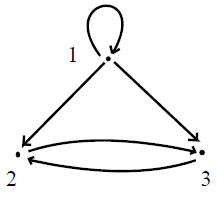
\includegraphics[scale=0.6]{images/10.png}

  Рис. 10 Представление марковской цепи в виде графа
\end{center}

На рисунке $10$ граф соответствует цепи с тремя состояними с ненулевыми следующими вероятностями, составляющие следующую матрицу такой цепи:
$$\begin{bmatrix}
	p_{11} & p_{12} & p_{13} \\
	0 & 0 & p_{23} \\
	0 & p_{32} & 0
\end{bmatrix}$$

Около дуг графа пишут значения вероятностей соответствующих переходов, вся информация, содержащаяся в матрице, переносится на граф.

Мы рассматривали вероятности перехода за $1$ шаг. Получи формулы для вероятностей перехода за несколько шагов.

Переход из состояния $i$ в состояние $j$ за два шага осуществляется следующим образом: за $1$ шаг переходим из $i$ в $k$ (промежуточное состояние), а потом за второй шаг из $k$ в $j$. таким образом, вероятность $p_{ij}^{(2)}$ перехода из $i$ в $j$ за $2$шага равна:
$$p_{ij}^{(2)} = \sum\limits_{k}p_{ik}\cdot p_{kj}$$
где суммирование ведется по всем состояниям $k$.

В общем случае переход из $i$ в $j$ за $m$ шагов можно разбить на два этапа: за первые $t$ шагов $0 < t < m$ осуществляется переход из $i$ в некоторое промежуточное состояние $k$, затем за оставшиеся $m-t$ шагов переход из $k$ в $j$. Вероятность $p_{ij}^{(m)}$ перехода из $i$ в $j$ за $m$ шагов:
$$p_{ij}^{(m)} = \sum\limits_{k}p_{ik}^{t} \cdot p_{kj}^{(m-t)}$$

При $t=1$ и $t=m-1$:
$$p_{ij}^{(m)} = \sum\limits_{k}p_{ik} \cdot p_{kj}^{(m-1)}$$
$$p_{ij}^{(m)} = \sum\limits_{k}p_{ik}^{m-1} \cdot p_{kj}$$

Эти формулы позволяют найти вероятности перехода за любое число шагов, если предварительно определеные вероятности перехода за меньшее число шагов.

\textbf{Пример:}

Дана матрица $P$ цепи Маркова с тремя состояними:
$$P = \begin{bmatrix}
	p_{11} & p_{12} & p_{13} \\
	p_{21} & p_{22} & p_{23} \\
	p_{31} & p_{32} & p_{33}
\end{bmatrix} = \begin{bmatrix}
	0 & \frac{1}{2} & \frac{1}{2} \\
	\frac{1}{3} & \frac{1}{3} & \frac{1}{3} \\
	\frac{1}{4} & \frac{1}{2} & \frac{1}{4}
\end{bmatrix}$$

Найти вероятность $p_{32}^{(3)}$, то есть вероятность перехода из $3$-его во $2$-е состояние за $3$ шага.

\begin{proof}
	Решение

	Согласно формуле для $t=1$ при $m=3$:
	$$p_{32}^{(3)} = \sum\limits_{k=1}^3 p_{3k} \cdot p_{k2}^{(2)} = p_{31}\cdot p_{12}^{(2)} + p_{32}\cdot p_{22}^{(2)} + p_{33}\cdot p_{32}^{(2)}$$

	Вероятности для второго шага:
	$$p_{12}^{(2)} = \sum\limits_{k=1}^3 p_{1k} \cdot p_{k2} = p_{11}\cdot p_{12} + p_{12}\cdot p_{22} + p_{13}\cdot p_{32} = \frac{5}{12}$$
	$$p_{22}^{(2)} = \sum\limits_{k=1}^3 p_{2k} \cdot p_{k2} = p_{21}\cdot p_{12} + p_{22}\cdot p_{22} + p_{23}\cdot p_{32} = \frac{4}{9}$$
	$$p_{32}^{(2)} = \sum\limits_{k=1}^3 p_{3k} \cdot p_{k2} = p_{31}\cdot p_{12} + p_{32}\cdot p_{22} + p_{33}\cdot p_{32} = \frac{5}{12}$$

	Следовательно:
	$$p_{32}^{(3)} = p_{31}\cdot p_{12}^{(2)} + p_{32}\cdot p_{22}^{(2)} + p_{33}\cdot p_{32}^{(2)} = \frac{31}{72}$$
\end{proof}

При фиксированном значении $m$ запись массива вероятностей $p_{ij}^{(m)}$ можно оформить в виде матрицы:
$$p^{(m)} = \begin{bmatrix}
		p_{11}^{(m)} & p_{12}^{(m)} & \ldots & p_{1n}^{(m)} \\
		p_{21}^{(m)} & p_{22}^{(m)} & \ldots & p_{2n}^{(m)} \\
		\ldots & \ldots & \ldots & \ldots \\
		p_{n1}^{(m)} & p_{n2}^{(m)} & \ldots & p_{nn}^{(m)}
	\end{bmatrix}$$

В этих обозначениях исходная матрица $P$ совпадает с $P^{(1)}$. Согласно правилу умножения и формуле $1.8$ вероятности за два шага, которая является ничем иным, как представление элемента при перемножении матриц при фиксированной строке и столбце, соответствующие индексу элементами. Поэтому, элементы матрицы $P^{(2)}$ совпадают с соответствующими элементами произведения матрицы $P$ на себя, так что $P^{(2)} = P^2$. 

\begin{remark}
	Верно следующее равенство:
	$$P^{(m)} = P^m$$
\end{remark}

\textbf{Утв:} матрица вероятностей перехода за $m$ шагов является стохастической.

\subsubsection{Финальные вероятности состояний и их вычисление}

Мы рассмотрели вероятности перехода из данного исходного состояние. Предположим, что исходное состояние нам не известно.

Пусть дано распределение вероятностей исходного состояния, то есть набор (стохастический вектор)
$$Q = (q_1,\ldots,q_n)$$
где $q_j$ - вероятность того, что исходным является $j$-е.

Свойства данного стохастического набора:
\begin{itemize}
	\item $0\leq q_j \leq 1$
	\item $\sum\limits_j q_j = 1$
\end{itemize}

Случай, когда исходное состояние полностью определено, соответствует тому, что одна из компонент вектора $Q$ равна $1$, а остальные равны $0$.

Пусть $q_j^{(m)}$ - вероятность того, что объект $S$ через $m$ шагов после начала функционирования окажется в $j$-м состоянии, если его начальное состояние задано вектором $(1.3)$, а вероятность перехода - матрицей $(1.2)$. Набор таких вероятностей обозначим посредством $Q^m$:
$$Q^{(m)} = (q_1^{(m)},q_2^{(m)},\ldots,q_n^{(m)})$$
при этом $Q = Q^{(0)}$ (0 шагов).

Нетрудно видеть, что:
$$q_j^{(m)} = \sum\limits_{k=1}^n q_kp_{kj}^{(m)}$$
то есть вероятность того, на $m$-м шаге окажется в $j$-м состоянии (вектор вероятностей $q$ на столбец вероятности $j$).

Откуда следует, что:
$$Q^{(m)} = Q \cdot P^{(m)}  = Q \cdot P^m$$

\textbf{Пример}

Дана матрица $P$ цепи Маркова с тремя состояними:
$$P = \begin{bmatrix}
	p_{11} & p_{12} & p_{13} \\
	p_{21} & p_{22} & p_{23} \\
	p_{31} & p_{32} & p_{33}
\end{bmatrix} = \begin{bmatrix}
	0 & \frac{1}{2} & \frac{1}{2} \\
	\frac{1}{3} & \frac{1}{3} & \frac{1}{3} \\
	\frac{1}{4} & \frac{1}{2} & \frac{1}{4}
\end{bmatrix}$$

и стохастический вектор вероятности того, что исходным является одно из $3$ состояний:
$$Q = \left(0,\frac{1}{4},\frac{3}{4}\right)$$

Найти вероятность того, что через $2$ шага после начала функционирования объет окажется во $2$ состоянии, то есть $q_2^{(2)}$:
$$q_2^{(2)} = \sum\limits_{k=1}^n q_kp_{k2}^{(2)} = q_1\cdot p_{12}^{(2)} +  q_2\cdot p_{22}^{(2)} + q_3\cdot p_{32}^{(2)} = \frac{61}{144}$$

\textbf{Обобщения}

Отметим два обобщения понятия марковской цепи.

\begin{enumerate}
	\item Первое связано с отказом от стационарности вероятностей перехода за один шаг, то есть элементы матрицы $P$ могут менять свои значения в зависимости от времени (числа шагов), прошедшего после начала функционирования. Такие цепи называются нестационарными.
	\item Второе связано с введением ограниченной зависимости от истории. Допускается, что зависимость вероятностей $p_{ij}$ от фиксированного $k$ состочний, предшествующих $i$. Такие цепи называются \textbf{$k$-связными}. При $k=0$ получаем обычную марковскую цепь.
\end{enumerate}

В дальнейшем мы будем рассматривать лишь стационарные обыкновенные цепи.

\newpage

\subsection{Марковские процессы}

Рассмотрим модификацию марковской цепи: откажемся от условия, что смена вероятностей возможна лишь в определенные дискретные моменты времени, то есть будем считать \textit{допустимой} смену состояний в любой момент.

\begin{definition}
	В такое случае говорят не о марковской цепи (дискретном процесса), а о \textbf{марковском процессе}.
\end{definition}

Различие между цепью и процессом связано с \textit{дискретностью или непрерывностью времени}. Множество состояний по-прежнему остается конечным или счетным, то есть дискретным.

Для процессов теряет смысл понятие перехода за один или несколько шагов, так как теряет смысл понятие шага. Матрица перехода заменяется матрицей:
$$P^{(t)} = \begin{bmatrix}
		p_{11}^{(t)} & p_{12}^{(t)} & \ldots & p_{1n}^{(t)} \\
		p_{21}^{(t)} & p_{22}^{(t)} & \ldots & p_{2n}^{(t)} \\
		\ldots & \ldots & \ldots & \ldots \\
		p_{n1}^{(t)} & p_{n2}^{(t)} & \ldots & p_{nn}^{(t)}
	\end{bmatrix}$$
где $p_{ij}^{(t)}$ есть вероятность перехода из $i$ в $j$ за время $t$.

Элементами этой матрицы являются не числа, а функции - конкректная числовая вероятность перехода получается при конкретизации времени $t$, за которое осуществляется переход.

Матрица переходов в непрерывном случае является стохастической, то есть $\forall t$ выполняются свойства стохастической матрицы:
\begin{itemize}
	\item $0\leq p_{ij}^{(t)} \leq 1$
	\item $\sum\limits_j p_{ij}^{(t)} = 1$
\end{itemize}

Вероятности перехода из состояния $i$ в состояние $j$ за время $t_1 + t_2$ можно выразить через вероятности переходов из состояния $i$ в различные другие промежуточные состояния $k$ за время $t_1$ и вероятности переходов из этих состояний $k$ в целевое состояние $j$ за время $t_2$. Соответствующая формула аналогична формуле для марковских цепей:
$$p_{ij}^{(t_1+t_2)} = \sum\limits_{k}p_{ik}^{(t_1)} \cdot p_{kj}^{(t_2)}$$

Матрицы вероятностей переходв за различные промежутки времени связаны между собой соотношением:
$$P^{(t_1+t_2)} = P^{(t_1)} \cdot P^{(t_2)}$$

Если дан вектор $Q$ вероятностей исходного состояния:
$$Q = (q_1,\ldots,q_n)$$
то вероятность $q_j^{(t)}$ того, что объект через время $t$ после начала окажется в состоянии $j$ может быть определен по формуле:
$$q_j^{(t)} = \sum\limits_{k=1}^n q_kp_{kj}^{(t)}$$

Таким образом, вектор $Q^{(t)}$ состояний через время $t$, компонентами которого являются $q_j^{(t)}$, удовлетворяет равенству:
$$Q^{(t)} = Q \cdot P^{(t)}$$

\newpage
\subsection{Процессы гибели и рождения}

Понятие марковского процесса является весьма плодотворным в
описании процессов обслуживания. Особенно важную роль при этом
играет частный случай марковских процессов – процессы гибели и
рождения. Эти процессы определяются следующим образом.

Для каждого состояния $i$ выделяется некоторое множество состояний $A_i$, содержащее $i$: состояния $j \in A_i$ называются состояниями, \textbf{соседними с состоянием $i$}.

\begin{definition}
	Марковский процесс называется процессом \textbf{гибели и рождения}, если вероятности перехода из одного состояния в другое удовлетворяют условиям:
	$$p_{ij}^{(t)} = o(t) \quad j \not \in A_i$$
	$$p_{ij}^{(t)} = a_{ij} \cdot t + o(t) \quad j \in A_i, j \neq i$$
	$$p_{ij}^{(t)} = 1- \sum\limits_{j \in A_i, j \neq i} \alpha_{ij} \cdot t + o(t)$$
\end{definition}

Первое условие показывает, что вероятность перехода не в соседнее состояние за малый промежуток времени есть величина, бесконечно малая по сравнению с длиной этого промежутка. Таким образом, переход не в соседнее состояние невозможен. 

Второе равенство позволяет выделить в вероятности перехода линейную часть.

Третье равенство дополняет сумму остальных до $1$.

В дальнейшем множество состояний будем нумеровать с $1$:
$$M = \{0,1,\ldots,n\}$$
$$M = \{0,1,\ldots,n\}$$
в случае конечного и бесконечного числа состояний.

Множество соседних состояний $A_i$ к состоянию $i$ будет определяться следующим образом:
$$A_i = \{i-1,i,i+1\}$$
при $i=0$ и при $i=n$:
$$A_0 = \{0,1\} \qquad A_n = \{n-1,n\}$$

Будем рассматривать далее обычное множество соседних состояний, не оговаривая каждый раз естественные изменения.

Равенства из определения при условии множества соседних состояний можно записать в следующем виде:
$$p_{ij}^{(t)} = o(t) \quad j<i-1 \quad j > i +1$$
$$p_{i,i-1}^{(t)} = a_{i,i-1} \cdot t + o(t)$$
$$p_{i,i+1}^{(t)} = a_{i,i+1} \cdot t + o(t)$$
$$p_{i,i}^{(t)} = 1 - a_{i,i-1} \cdot t - a_{i,i+1} \cdot t + o(t)$$

Для коэффициентов $\alpha$ приняты специальные обозначения:
$$a_{i,i-1} = v_i \quad  a_{i,i+1} = \lambda_i$$
так что:
$$p_{i,i-1}^{(t)} = v_i \cdot t + o(t)$$
$$p_{i,i+1}^{(t)} = \lambda_i \cdot t + o(t)$$
$$p_{i,i}^{(t)} = 1 - (v_i + \lambda_i) \cdot  t + o(t)$$

\begin{center}
  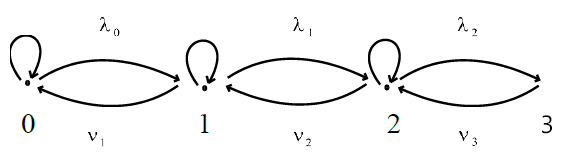
\includegraphics[scale=0.5]{images/11.png}

  Рис. 11 Граф непосредственных переходов
\end{center}

Величины $\lambda_i$ и $v_i$ не являются вероятностями переходов, они лишь управляют вероятностями, являясь коэффициентами в соответствующих выражениях. Эти величины неотрицательны. Может оказаться, что некоторые из них равны $0$.

\begin{definition}
	Если $\lambda_i = 0$, то процесс называется процессом \textbf{чистой гибели}. В соответствующем графе возможны переходы только налево (в состояние с меньшим либо равным номером). Через некоторое время процесс приходит в граничное нулевое состояние, в котором зацикливается.
\end{definition}

\begin{definition}
	Если $v_i = 0$, то процесс называется процессом \textbf{чистого рождения}. Он разворачивается только направо и уходит по последовательности состояний в бесконечность.
\end{definition}

Свое название такие процессы получили в связи с тем, что впервые
они были применены к биологическим проблемам изучения динамики
популяции, распространения эпидемий и другим. Если номер состояния
интерпретировать как число индивидов в популяции, то переход направо
соответствует рождению, а налево - гибели одного из индивидов.

В дальнейшем процессы гибели и рождения нашли важное
применение в экономике, технике и других областях знания. Как мы
увидим далее, они играют фундаментальную роль в моделировании
процессов обслуживания.

В случае конечного числа состояний процесс чистого рождения, удовлетворяющий условиям множества соседних событий, можно заменить процессом чистой гибели, удовлетворяющим тем же условиям и наоборот.

\subsubsection{Задача об агрегате}

В станке имеются два одинаковых дублирующих друг друга узла. Если работают оба узла, то для каждого из них вероятность бесеребойной работыв течение времени $t$ равна:
$$P(t_w \geq t) = e^{-\lambda t}$$

Если один из узлов сломался, то станок продолжает работать, но ввиду увеличения нагрузки на оставшийся узел вероятность его бесперебойной работы в течение времени $t$ определяется другой формулой и равна:
$$P(t_w \geq t) = e^{-3\lambda t}$$

Ремонтный рабочий ремонтирует сломанный узел, причем вероятность того, что время ремонта займет не меньше $t$ равна:
$$P(t_{\text{рем}} \geq t) = e^{-v t}$$

Если сломаны два узла, то они ремонтируются по очереди. Требуется описать функционирование этой системы в терминах марковских процессов и найти вероятности переходов.
\begin{proof}
	Решение:

	Введем три состояния: $0,1,2$ по числу сломанных узлов.

	Экспоненциальный закон распределения обеспечивает отсутствие последействия в функционировании нашей системы. Таким обращом, функционирование описывается марковским процессом. Найдем вероятности переходов.

	Переход $0 \to 1$ означает поломку одного из двух узлов, переход в ситуацию, когда один из узлов сломан, а другой продолжает работать:
	$$P_{0,1}^{(t)} = 2 \cdot (1-e^{-\lambda t}) \cdot e^{-\lambda t} = 2 \cdot (\lambda t + o(t)) \cdot (1-\lambda t + o(t)) = 2\lambda t + o(t)$$

	Переход $1 \to 2$ означает поломку оставшегося узла при условии, что сломанный ранее узел не успели отремонитровать:
	$$P_{1,2}^(t) = (1-e^{-3\lambda t}) \cdot  e^{-v t} = (3\lambda t + o(t)) \cdot (1-vt +o(t)) = 3\lambda t + o(t)$$

	Для вероятности перехода $0 \to 2$ можно написать равенство:
	$$P_{0,2}^{(t)} \leq (1-e^{-\lambda t})^2 = o(t)$$
	то есть вероятность того, что оба станка сломаются очень маленькая по сравнению с промежутком времени $t$.

	Аналогично:
	$$P_{2,1}^{(t)} = 1-e^{-vt} = vt +o(t)$$
	$$P_{1,0}^{(t)} = (1-e^{-vt}) \cdot  e^{-3\lambda t}$$
	$$P_{2,0}^{(t)} \leq (1-e^{-vt})^2 = o(t)$$

	Перед нами процесс гибели и рождения с $N=3$, соответствующим условиям. При этом:
	$$\lambda_0 = 2\lambda, \lambda_1 = 3\lambda, v_2 = v_1 = v$$

	Посчитаем вероятности нахождения в состояних:
	$$p_{0,0}^{(t)} = e^{-\lambda t}e^{-\lambda t} = 1 - 2\lambda t + o(t)$$
	что соответствует условию:
	$$p_{0,0}^{(t)} = 1 - (v_0 + \lambda_0) \cdot  t + o(t) = 1 -2\lambda t $$
	$$p_{1,1}^{(t)} = e^{-3\lambda t}e^{-v t} = 1 -(3\lambda +v)t + o(t)$$
	что соответствует работе станка нагруженно при непочинке нерабочего станка
	$$p_{1,1}^{(t)} = 1 - (v_1 + \lambda_1) \cdot  t + o(t) = 1 -(v + 3\lambda) t +o(t)$$
	$$p_{2,2}^{(t)} = 1 - (v_2 + \lambda_2) \cdot  t + o(t) = 1 - v\cdot  t +o(t)$$
	
\end{proof}

\subsubsection{Задача о станке-автомате}

На станок автомат каждую минуту может поступить деталь одного из двух типов. Время обработки первой детали  - $1$ минута, второго типа - $2$ минуты. Если деталь поступает тогда, когда станов занят, то она получает отказ и переходит на другой станок. Вероятность поступления детали в очередную минуту равна $p$, вероятнотсть отсутствия - $q$. Вероятности того, что поступившая деталь окажется деталью первого ии второго типа равны $b_1$ и $b_2$ соответственно.

\textbf{Найти:} доли времени, когда станок занят обработкой и когда он свободен.
\begin{proof} Решение

	Опишем функционирование в терминах марковской цепи.

	Введем три состояния: $0$ - станок свободен (деталь не поступила), $1$ - станок заняет и оставшееся время обработки равно $1$ минуте (как деталь первого, так и деталь второго), $2$ - станок занят и оставшееся время обработки равно $2$ минутам.

	$p_{00} = q$ - вероятность того, что станок из состояния $0$ перейдет в состояние $0$, то есть равна вероятности непоступления детали.

	$p_{10} = q$ - так как если станок находился в состоянии $1$, то к следующей минуте он окончил работу и освободится, а вероятность того, что он останется свободным равна $q$.

	$p_{01} = pb_1$ - вероятность поступления детали первого типа умноженную на вероятность поступления детали в принципе.

	$p_{11} = pb_1$ - вероятность поступления детали первого типа, умноженную на вероятность поступления детали в принципе.

	$p_{02} = p_{12} = pb_2$

	$p_{20} = p_{22} = 0$

	$p_{21} = 1$

	Таким образом, матрица переходов:
	$$\begin{bmatrix}
		q & pb_1 & pb_2 \\
		q & pb_1 & pb_2 \\
		0 & 1 & 0 \\
	\end{bmatrix}$$

	Финальные вероятности есть следующая система векторов:
	$$\begin{cases}
		p_0 = qp_0 + qp_1 \\
		p_1 = pb_1 \cdot p_0 + pb_1 \cdot p_1 + p_2 \\
		p_2 = pb_2 \cdot p_0 + pb_2 \cdot p_1 \\
		p_0 + p_1 + p_2 =  1
	\end{cases}$$

	Решением данной системы является:
	$$p_0 = \frac{q}{1+pb_2} \qquad p_1 = \frac{p}{1+pb_2} \qquad p_2 = \frac{pb_2}{1+pb_2}$$

	Доля времени, когда станок свободен  - $p_0$, доля времени, когда станок занят - $p_1+p_2$.
\end{proof}

\newpage
\subsection{Финальные вероятности состоний для процессов гибели и рождения}

Будем рассматривать процесс с бесконечным числом состояний, удовлетворяющие условиям множества соседних событий.

Обозначим $P_k(t)$ - вероятность того,что процесс через время $t$ после своего начала окажется в состоянии $k$. Сформулируем уравнения для таких вероятностей.

Рассмотрим два момента времени $t$ и $t + \tau$. За небольшой промежуток времени $\tau$ процесс мог попасть в $k$ лишь из соседних состояний. Для $k \geq 1$:
$$P_k(t + \tau) = \sum\limits_{i=0}^{\infty}P_i(t) \cdot p_{ik}^{(\tau)} = P_{k-1}(t) \cdot p_{k-1,k}^{(\tau)} +  P_{k}(t) \cdot p_{k,k}^{(\tau)} +  P_{k+1}(t) \cdot p_{k+1,k}^{(\tau)} = $$
$$ =  P_{k-1}(t) \cdot (\lambda_{k-1} \cdot \tau+ o(\tau)) + P_k(t) \cdot (1 - (v_k + \lambda_k) \cdot  \tau + o(\tau)) + P_{k+1}(t) \cdot ( v_{k+1} \cdot \tau + o(\tau)) + o(\tau)$$

Преобразуем данное выражение и устремими $\tau \to 0$:
$$\frac{P_k(t + \tau)  - P_k(t)}{\tau} = \lambda_{k-1} \cdot P_{k-1}(t) -(v_k + \lambda_k)P_k(t) + v_{k+1} \cdot P_{k+1}(t) + \frac{o(\tau)}{\tau}$$
$$P_k'(t) = \lambda_{k-1} \cdot P_{k-1}(t) -(v_k + \lambda_k) \cdot P_k(t) + v_{k+1} \cdot P_{k+1}(t)$$
получаем дифференциальное уравнение, которое можно рассматривать как систему уравнений. Все члены этого уравнения осмыслены лишь при $k \geq 1$, при $k=0$ возникают неосмысленные выражения, но можно провести отдельно вывод для $k=0$, получив:
$$P_0'(t) = -\lambda_0 \cdot P_0(t) + v_1 \cdot P_1(t)$$

Если множество состояний конечно и $v_i,\lambda_i$ отличны от $0$, то для последнего состояния $n$ по аналогичным причинам уравнение принимает вид:
$$P_n'(t) = -\lambda_{n-1} \cdot P_{n-1}(t) + v_n \cdot P_n(t)$$

Можно доказать, что:
$$\lim\limits_{t \to \infty} P_k(t) = P_k > 0$$

Для любого $t$:
$$\sum\limits_{k=0}^n P_k(t) = 1$$
так что в пределе получаем такое же соотношение финальных вероятностей:
$$\sum\limits_{k=0}^n P_k = 1$$

Если число состояний бесконечно, то строгая положительность $v_i, \lambda_i$ не гарантирует выполнения аналогичных равенств, может оказаться, что
$$\sum\limits_{k=0}^n P_k(t) < 1$$

Это может быть связано с тем, что процесс в своем движении по
состояниям направо за ограниченное время $t$ проходит бесконечно
большое число состояний. 

\begin{definition}
	Такой процесс описывает явление \textbf{типа "взрыва".}
\end{definition}

\begin{theorem}
	Для того, чтобы существовали пределы $\lim\limits_{t \to \infty} P_k(t) = P_k > 0$ для любого $t$ и выполнялось равенство:
	$$\sum\limits_{k=0}^{\infty} P_k(t) = 1$$
	достаточно выполнения следующего условия: существует такая величина $\beta$, что для всех $k$, начиная с некоторого, выполнено неравенство:
	$$\frac{\lambda_k}{v_{k+1}} \leq \beta <1$$
\end{theorem}

То есть начиная с некоторого $k$ передвигаться по состояниям налево становится легче, чем направо , что и предотвращает взрыв. В ТМО это условие обычно (но не всегда) выполнено, так что существуют финальные вероятности, дающие в сумме $1$, то есть существует установившийся режим работы системы обслуживания.

\begin{theorem}
	Найдем финальные вероятности в предположении, что они существуют
\end{theorem}
\begin{proof}
	Перейдем к пределу в дифференциальных уравнениях при $t \to \infty$. Пределы левых частей уравнений существуют, так как существуют пределы правых.

	Пусть $\lim\limits_{t \to 0} P_k'(t) = c_k$. Тогда $c_k = 0 \forall k$. 

	То есть предел производных равен $0$ и переход к пределу дает систему линейных алгебраических уравнений:
	$$\begin{cases}
		\lambda_{k-1} \cdot P_{k-1}(t) -(v_k + \lambda_k) \cdot P_k(t) + v_{k+1} \cdot P_{k+1}(t) = 0\\
		-\lambda_0 \cdot P_0(t) + v_1 \cdot P_1(t) = 0
	\end{cases}$$

	Обозначим за $x_{k+1} = -\lambda_k P_k + v_{k+1}P_{k+1}$, тогда:
	$$\begin{cases}
		x_{k+1} - x_k = 0 \\
		x_1 = 0
	\end{cases}$$

	Следовательно $x_{k+1} = x_k = \ldots = x_{1} = 0$, то есть единственным решением является $x_k = 0$ для $k \geq 1$. Получаем для любого $k \geq 1$:
	$$x_{k} = -\lambda_{k-1} P_{k-1} + v_{k}P_{k}  = 0$$
	$$P_k =\frac{\lambda_{k-1}}{v_k} \cdot P_{k-1} \qquad P_{k-1} =\frac{\lambda_{k-2}}{v_{k-1}} \cdot P_{k-2} \qquad P_1 = \frac{\lambda_0}{v_1} \cdot P_0$$

	Отсюда получаем:
	$$P_k = \frac{\lambda_{k-1}}{v_k} \cdot \frac{\lambda_{k-2}}{v_{k-1}} \cdot \ldots \cdot \frac{\lambda_0}{v_1} \cdot P_0 = \prod_{i=1}^k \frac{\lambda_{i-1}}{v_i} \cdot P_0$$

	Мы выразили все финальные вероятности $P_k$ через $P_0$. Вероятность $P_0$ найдем из нормирующего условия:
	$$\sum\limits_{k=0}^{\infty} P_k = 1$$
	$$\sum\limits_{k=0}^{\infty} \prod_{i=1}^k \frac{\lambda_{i-1}}{v_i} \cdot P_0 = 1$$
	$$P_0 = \frac{1}{1+ \sum\limits_{k=1}^{\infty} \prod\limits_{i=1}^k \frac{\lambda_{i-1}}{v_i}}$$

	Откуда для $j \geq 1$ получаем окончательные формулы для финальных вероятностей $p_j$:
	$$P_j = \frac{ \prod\limits_{i=1}^j \frac{\lambda_{i-1}}{v_i}}{1+ \sum\limits_{k=1}^{\infty} \prod\limits_{i=1}^k \frac{\lambda_{i-1}}{v_i}}$$
\end{proof}

Формулы позволяют выразить финальные вероятности состояний через параметры вероятностей переходов из одного состояния в другое. При практических расчетах удобнее использовать формулу:
$$P_k = \frac{\lambda_{k-1}}{v_k} \cdot \frac{\lambda_{k-2}}{v_{k-1}} \cdot \ldots \cdot\frac{\lambda_0}{v_1} \cdot P_0 = \prod_{i=1}^k \frac{\lambda_{i-1}}{v_i} \cdot P_0$$
позволяющую выразить искомые вероятности через одну и ту же вероятность $P_0$ вместе с формулой 
$$P_0 = \frac{1}{1+ \sum\limits_{k=1}^{\infty} \prod\limits_{i=1}^k \frac{\lambda_{i-1}}{v_i}}$$
позволяющей определить саму вероятность $P_0$.

\textbf{Пример:}

Выведем финальные вероятности для задачи об агрегате:
\begin{proof}
	Напомним результаты, которые мы получили:

	Перед нами процесс гибели и рождения с $N=3$, соответствующим условиям. При этом:
	$$\lambda_0 = 2\lambda, \lambda_1 = 3\lambda, v_2 = v_1 = v$$

	Тогда:
	$$P_0 = \frac{1}{1+\frac{\lambda_0}{v_1} + \frac{\lambda_0\lambda_1}{v_1v_2} + \frac{\lambda_0\lambda_1\lambda_2}{v_1v_2v_3}} = \frac{2\lambda}{v} + \frac{6\lambda^2}{v^2}$$
	$$\lambda_i \quad i \geq n \qquad  v_i = 0 \quad i\geq n+1$$
	$$P_1 =  \prod_{i=1}^1 \frac{\lambda_{i-1}}{v_i} \cdot P_0 = \frac{\lambda_0}{v_1}P_0 = \frac{4\lambda^2(v+3\lambda)}{v^3}$$
	$$P_2 =  \prod_{i=1}^2 \frac{\lambda_{i-1}}{v_i} \cdot P_0 = \frac{\lambda_0}{v_1} \cdot \frac{\lambda_1}{v_1} \cdot P_0 = \frac{12\lambda^3(v+3\lambda)}{v^4}$$
\end{proof}

\newpage
\subsection{СМО с отказанием}

Мы рассмотрим в этом параграфе систему обслуживания, удовлетворящему следующим:

\begin{enumerate}
	\item Если в момент поступления требования имеется хотя бы один свободный узел обслуживания, то требование сразу начинает обслуживаться (любым из свободных узлов)
	\item Каждый узел в любой момент времени обслуживает не более одного требования
	\item Каждое требование обслуживается одним узлом 
	\item Обслуживание не прерывается
	\item По окончании обслуживания требование покидает систему
	\item Входящий поток является пуассоновским
	\item Продолжительность обслуживания является случайной величиной, распределенной по экспоненциальному закону, одному и тому же для всех узлов обслуживания - узлы предполагаются \textit{одинаковыми} по \textit{вероятностным характеристикам}, причем вероятность тго, что время обслуживания больше заданного времени $t$ равна:
	$$P(t_{\text{обл}} > t) = e^{-vt}$$
	где $v$ - интенсивность обслуживания - среднее число требования, обслуживаемых узлом в единицу времени.
\end{enumerate}

Такой системой обслуживания является \textbf{телефонная станция}. Исследовалась датским ученым \textit{А.К.Эрлангом}.

\subsubsection{Функционирование системы как процесс гибели и рождения}

Пусть $\lambda$ - параметр входящего пуассоновского потока требования. Пусть $N \geq 1$ - число узлов обслуживаний. Опишем функционирование СМО в терминах процессов гибели и рождения.

Для этого необходимо:

\begin{itemize}
	\item Ввести понятие состояния
	\item Обосновать, что процесс перехода из состояния в состояние является марковским 
	\item Доказать, что вероятности перехода удовлетворяют условиям процессов гибели и рождения
\end{itemize}

\textbf{1. Формализация понятия состояния}

\begin{definition}
	\textbf{Состоянияем СМО с отказами} назовем число требований, находящихся в системе, то есть число требований, находящихся в узлах обслуживания. 

	Состояними являются целые неотрицательные числа в пределах от $0$ до $N$:
	$$\{0,1,\ldots,N\}$$
\end{definition}

\textbf{2. Процесс функционирования является марковским}

Действительно, пусть в момент времени $t$ состоянием является $i$, в момент $t + \tau$ состоянием является $j$. Изменение состояния (изменение числа требований), находящихся в системе обслуживания, имеет две причины:
\begin{enumerate}
	\item Поступление новых требований из входящего потока - так как входящий поток пуассоновский, то поступление требований на любом отрезке не зависит от истории потока до начального момента этого отрезка (отсутствие последействия в пуассоновском потоке). Оно не зависит и от требований, поикдающих систему. Таким образом, изменение состояния о первой причине облажает марковским свойством
	\item Уход обслуженных требований - если в момент времени $t$ требование уже обслуживалось, то вероятность окончания обслуживания до момента $t + \tau$ не зависит от того, сколько длилось обслуживание до момента $t$. Это обстоятельство связано с экспоненциальностью распределения длительности обслуживания (отсутствие памяти). Рассматривая интервал между началом и окончанием обслуживания, мы можем убедиться в этом. Таким образом, данной свойство также обладает марковским свойством и процесс функционирования является марковским.
\end{enumerate}

\textbf{3. Вероятности переходов из одного состояния в другое}

Переход из $i \to i+1$ за $t$ связан с поступлением одного требования в систему за это требование и уходом нуля требований (с тем, что ни один из занятых узлов за это время обслуживания не закончил).

Число занятых узлов равно $i$ умноженную на вероятность поступления одного требования
$$P_{i,i+1}^{(t)} = e^{-\lambda t} \cdot \lambda t \cdot e^{-ivt} = \lambda t (1-\lambda t + o(t))(1-ivt+o(t)) = \lambda t + o(t)$$

Переход $i \to i-1$ связан с поступлением нуля требований и уходом одного (ровно один из занятых узлов окончил обслуживание):
$$P_{i,i-1}^{(t)} = e^{-\lambda t}\cdot C_i^1 (1-e^{-vt})\left(e^{-vt}\right)^{i-1} = ivt + o(t)$$

Переход $i \to i$ связан с отсутствием поступления требований в систему и уходу требований из системы. Такой переход имеет вероятность:
$$P_{i,i}^{(t)} = e^{-\lambda t}\cdot e^{-ivt} = 1 - \lambda t - ivt +o(t)$$

Все остальные вероятности переходов величины бесконечно малые.

При определении вероятностей мы учли не все возможные случаи. Например, переход $i \to i +1$ возможен не только при поступлении одного, но и при поступлении $n$ требований и уходе $n-1$ требований, но вероятности таких событий при $n \geq 2$ (и их сумма) являются бесконечно малыми, единственный существенный вклад в эту вероятность даст случай, учтенный выше - $n=0$.

Мы убедились, что вероятности переходов удовлетворяют условиям процессов гибели и рождения. При этом коэффициенты $\lambda_i$ и $v_i$, характеризующие процессы, определяются формулами:
$$ \lambda_i  = \lambda$$
$$v_i = iv$$
по определению процессов гибели и рождения.

\subsubsection{Финальные вероятности состояний}

Воспользуемся формулой финальных вероятностей для процессов гибели и рождения:
$$P_k = \frac{\lambda_{k-1}}{v_k} \cdot \frac{\lambda_{k-2}}{v_{k-1}} \cdot \ldots \cdot \frac{\lambda_0}{v_1} \cdot P_0 = \prod_{i=1}^k \frac{\lambda_{i-1}}{v_i} \cdot P_0 = \frac{\lambda}{kv} \cdot \frac{\lambda}{(k-1)v} \cdot \ldots \cdot \frac{\lambda}{1\cdot v} \cdot P_0 = \frac{\lambda^k}{v^k k!} P_0$$

\begin{definition}
	Величина $\rho = \frac{\lambda}{v}$ является отношением интенсивности входящего потока к интенсивности осблуживания и называется \textbf{загрузкой системы}.

	Данная величина является безразмерной и, в отличие от $\lambda$ и $v$, она не зависит от того, какой интервал времени выбран в качестве единицы. $\rho$ является естественной и важной характеристикой систем обслуживания и через нее выражаются многие другие характеристики
\end{definition}

Подставим в формулу вероятностей $P_k(t)$:
$$P_k = \frac{\rho^k}{k!} \cdot P_0$$

Так как $\sum\limits_{k=0}^N P_k = 1$, то:
$$P_0 = \frac{1}{\sum\limits_{k=0}^N \frac{\rho^k}{k!}}$$
и отсюда имеем формулы любых вероятностей:
$$P_j = \frac{\frac{\rho^j}{j!}}{\sum\limits_{k=0}^N \frac{\rho^k}{k!}}$$

Эти формулы носят название \textbf{формул Эрланга}. Эти формулы верны для СМО с отказами при любом законе распределения длительности обслуживания, при интенсивности обслуживания, равной $v$.

\subsubsection{Важнейшие характеристики функционирования системы}

\textbf{1. Вероятность отказа}

Требование, поступающее в систему, получает отказ в том и только том случае, когда все узлы заняты. Поэтому вероятность отказа $P_{\text{отк}}$ равна:
$$P_{\text{отк}} = P_N = \frac{\frac{\rho^N}{N!}}{\sum\limits_{k=0}^N \frac{\rho^k}{k!}}$$

\begin{definition}
	\textbf{Вероятность отказа} $P_{\text{отк}}$ характеризует долю требований, получающих отказ.
\end{definition}

\begin{definition}
	Величина
	$$\alpha = 1 - P_{\text{отк}} = 1 - P_N$$
	определяется долю обслуженных требованийи называется \textbf{относительной пропускной способностью} СМО.
\end{definition}

\begin{definition}
	\textbf{Абсолютная пропускная способность системы} - среднее число требований, поступающих в узлы осблуживания за единицу времени:
	$$A = \lambda \cdot (1-P_N) = \lambda \cdot \alpha$$
\end{definition}

\begin{definition}
	\textbf{Среднее число занятых узлов обслуживания $M_{\text{зан}}$} равна:
	$$M_{\text{зан}} = \sum\limits_{k=0}^N k \cdot P_k = \sum\limits_{k=1}^N k \cdot \frac{\rho^k}{k!} \cdot P_0 = \rho \cdot \sum\limits_{m=0}^{N-1} \frac{\rho^m}{m!} \cdot P_0 = $$
	$$ = \rho \cdot \sum\limits_{m=0}^{N-1} \frac{\rho^m}{m!}\cdot  \frac{1}{\sum\limits_{k=0}^N \frac{\rho^k}{k!}} = \rho\cdot \frac{\sum\limits_{k=0}^{N} \frac{\rho^k}{k!} - \frac{\rho^N}{N!}}{\sum\limits_{k=0}^N \frac{\rho^k}{k!}} = $$
	$$ = \rho \cdot \left(1- \frac{\frac{\rho^N}{N!}}{\sum\limits_{k=0}^N \frac{\rho^k}{k!}}\right) = \rho \cdot (1-P_N)$$
\end{definition}
\begin{definition}
	\textbf{Среднее число свободных узлов} $M_{\text{св}}$ равно разности:
	$$M_{\text{св}} = N - M_{\text{зан}}$$
\end{definition}

Для случая, когда в СМО с отказами имеется всего один узел обслуживания, мы получаем:
$$P_0 =  \frac{1}{\sum\limits_{k=0}^{1} \frac{\rho^k}{k!}} = \frac{1}{1+\rho}$$
$$P_{\text{отк}} = P_1 =  \frac{\rho}{1+\rho}$$
$$M_{\text{зан}} = \rho \cdot (1- P_N ) = \rho \cdot(1-P_1) = \rho \cdot \left (1 -  \frac{\rho}{1+\rho}\right) = \frac{\rho}{1+\rho}$$

Для случая, когда в СМО с отказами имеется всего два узла обслуживания, мы получаем:
$$P_0 =  \frac{1}{\sum\limits_{k=0}^{2} \frac{\rho^k}{k!}} = \frac{1}{1+\rho+\frac{\rho^2}{2}}$$
$$P_{\text{отк}} = P_2 =  \frac{\frac{\rho^2}{2!}}{1+\rho+\frac{\rho^2}{2}}$$
$$M_{\text{зан}} = \rho \cdot (1- P_N ) = \rho \cdot(1-P_2) = \rho \cdot \left (1 -   \frac{\frac{\rho^2}{2!}}{1+\rho+\frac{\rho^2}{2}}\right) = \frac{\rho}{1+\rho} = \frac{2\rho \cdot (1-\rho)}{2+\rho(2+\rho)}$$

Если число узлов велико по сравнению с загрузкой системы, то $N = \infty$. 

\begin{theorem}
	Для систем с бесконечным числом узлов:
	$$P_0 = e^{-\rho}$$
	$$P_k = \frac{\rho^k}{k!} \cdot e^{-\rho}$$
	$$M_{\text{зан}} =\rho$$
\end{theorem}
\begin{proof}
	$$P_0 = \frac{1}{\sum\limits_{k=0}^{\infty} \frac{\rho^k}{k!}} = \frac{1}{e^{\rho}} = e^{-\rho}$$
	$$P_k = \frac{\rho^k}{k!} \cdot P_0 = \frac{\rho^k}{k!} \cdot e^{-\rho}$$

	При $N \to \infty$ $P_N \to 0$:
	$$M_{\text{зан}} = \rho (1-P_N) = \rho$$
\end{proof}

\newpage
\subsection{СМО с ожиданием}

Мы рассмотрим в этом параграфе систему обслуживания с накопителем, удовлетворяющую следующим условиям:

\begin{enumerate}
	\item Если в момент поступления требования имеется хотя бы один свободный узел обслуживания, то требование сразу начинает обслуживаться (любым из свободных узлов)
	\item Если все узлы заняты, то поступившее требование становится в очередь за уже имеющимся в накопителе требованиям
	\item Если в момент освобождения узла имеется хотя бы одно требование в накопителе, то первое из них по очереди сразу поступает на обслуживание 
	\item Каждый узел в любой момент времени обслуживает не более одного требования
	\item Каждое требование обслуживается одним узлом 
	\item Обслуживание не прерывается
	\item По окончании обслуживания требование покидает систему
	\item Входящий поток является пуассоновским
	\item Продолжительность обслуживания является случайной величиной, распределенной по экспоненциальному закону, одному и тому же для всех узлов обслуживания - узлы предполагаются \textit{одинаковыми} по \textit{вероятностным характеристикам}, причем вероятность тго, что время обслуживания больше заданного времени $t$ равна:
	$$P(t_{\text{обл}} > t) = e^{-vt}$$
	где $v$ - интенсивность обслуживания - среднее число требования, обслуживаемых узлом в единицу времени.
\end{enumerate}

Из $2-3$ условий следует, что очередь в накопителе упорядочена естественным образом, не предусматривается, что требования обладают приоритетом перед другими. Любой узел доступен непосредственно из накопителя, то есть узлы работают не последовательно, а параллельно. Свободные узлы - пустой накопитель.

Из $4-6$ - требования обслуживаются независимо и узлы работают независимо. 

$7$ - разомкнутость системы.

\subsubsection{Функционирование системы как процесс гибели и рождения}

Пусть $\lambda$ - параметр входящего пуассоновского потока требования. Пусть $N \geq 1$ - число узлов обслуживаний. Опишем функционирование СМО в терминах процессов гибели и рождения.

Для этого необходимо:

\begin{itemize}
	\item Ввести понятие состояния
	\item Обосновать, что процесс перехода из состояния в состояние является марковским 
	\item Доказать, что вероятности перехода удовлетворяют условиям процессов гибели и рождения
\end{itemize}

\textbf{1. Формализация понятия состояния}

\begin{definition}
	\textbf{Состоянияем СМО с отказами} назовем число требований, находящихся в системе, то есть сумму числа требований в узлах и числа требований в накопителе.

	При этом $0$ соответствует отсутствию требований в системе, состояние $k$ при $k \leq N$ соответствуют отсутствию очереди, при $k \geq N$ - занятость всех узлов, а при $k > N$ - еще и наличие очереди.
\end{definition}

\textbf{2. Процесс функционирования является марковским}

Действительно, пусть в момент времени $t$ состоянием является $i$, в момент $t + \tau$ состоянием является $j$. Изменение состояния (изменение числа требований), находящихся в системе обслуживания, имеет две причины:
\begin{enumerate}
	\item Поступление новых требований из входящего потока - так как входящий поток пуассоновский, то поступление требований на любом отрезке не зависит от истории потока до начального момента этого отрезка (отсутствие последействия в пуассоновском потоке). Оно не зависит и от требований, поикдающих систему. Таким образом, изменение состояния о первой причине облажает марковским свойством
	\item Уход обслуженных требований - если в момент времени $t$ требование уже обслуживалось, то вероятность окончания обслуживания до момента $t + \tau$ не зависит от того, сколько длилось обслуживание до момента $t$. Это обстоятельство связано с экспоненциальностью распределения длительности обслуживания (отсутствие памяти). Рассматривая интервал между началом и окончанием обслуживания, мы можем убедиться в этом. Таким образом, данной свойство также обладает марковским свойством и процесс функционирования является марковским.
\end{enumerate}

\textbf{3. Вероятности переходов из одного состояния в другое}

Переход из $i \to i+1$ за $t$ связан с поступлением одного требования в систему за это требование и уходом нуля требований (с тем, что ни один из занятых узлов за это время обслуживания не закончил).

Число занятых узлов равно $i$ при $i \leq N$ и равно $N$ при $i \geq N$. При $i \leq N$ имеем:
$$P_{i,i+1}^{(t)} = e^{-\lambda t} \cdot \lambda t \cdot e^{-ivt} = \lambda t (1-\lambda t + o(t))(1-ivt+o(t)) = \lambda t + o(t)$$

Аналогично при $i \geq N$: 
$$P_{i,i+1}^{(t)} = \lambda t \cdot e^{-\lambda t} \cdot (e^{-vtN}) = \lambda t(1-\lambda t +o(t)) \cdot (1-Nvt +o(t)) = \lambda t + o(t)$$

Переход $i \to i-1$ связан с поступлением нуля требований и уходом одного (ровно один из занятых узлов окончил обслуживание). При $i \leq N$:
$$P_{i,i-1}^{(t)} = e^{-\lambda t}\cdot C_i^1 (1-e^{-vt})\left(e^{-vt}\right)^{i-1} = ivt + o(t)$$

При $i \geq N$:
$$P_{i,i-1}^{(t)} = e^{-\lambda t}\cdot C_N^1 (1-e^{-vt})\left(e^{-vt}\right)^{N-1} = Nvt + o(t)$$

Переход $i \to i$ связан с отсутствием поступления требований в систему и уходу требований из системы. Такой переход имеет вероятность при $i \leq N$:
$$P_{i,i}^{(t)} = e^{-\lambda t}\cdot e^{-ivt} = 1 - \lambda t - ivt +o(t)$$

При $i \leq N$:
$$P_{i,i}^{(t)} = e^{-\lambda t} \cdot (e^{-vt})^N = 1-\lambda t - Nvt +o(t)$$

Все остальные вероятности переходов величины бесконечно малые.

При определении вероятностей мы учли не все возможные случаи. Например, переход $i \to i +1$ возможен не только при поступлении одного, но и при поступлении $n$ требований и уходе $n-1$ требований, но вероятности таких событий при $n \geq 2$ (и их сумма) являются бесконечно малыми, единственный существенный вклад в эту вероятность даст случай, учтенный выше - $n=0$.

Мы убедились, что вероятности переходов удовлетворяют условиям процессов гибели и рождения. При этом коэффициенты $\lambda_i$ и $v_i$, характеризующие процессы, определяются формулами:
$$ \lambda_i  = \lambda$$
$$v_i = \begin{cases}
	iv, i \leq N \\
	Nv, i \geq N
\end{cases}$$
по определению процессов гибели и рождения.

\subsubsection{Финальные вероятности состояний}

Воспользуемся формулой финальных вероятностей для процессов гибели и рождения. При $k \leq N$
$$P_k = \frac{\lambda_{k-1}}{v_k} \cdot \frac{\lambda_{k-2}}{v_{k-1}} \cdot \ldots \cdot \frac{\lambda_0}{v_1} \cdot P_0 = \prod_{i=1}^k \frac{\lambda_{i-1}}{v_i} \cdot P_0 = \frac{\lambda}{kv} \cdot \frac{\lambda}{(k-1)v} \cdot \ldots \cdot \frac{\lambda}{1\cdot v} \cdot P_0 = \frac{\lambda^k}{v^k k!} P_0$$

При $k \geq N$:
$$P_k = \frac{\lambda}{Nv} \cdot \ldots \cdot  \frac{\lambda}{Nv} \cdot  \frac{\lambda}{Nv} \cdot  \frac{\lambda}{(N-1)v} \cdot \ldots \cdot  \frac{\lambda}{1v} \cdot P_0 = \frac{\lambda^k}{v^k \cdot N! \cdot N^{k-N}} \cdot P_0$$

\begin{definition}
	Величина $\rho = \frac{\lambda}{v}$ является отношением интенсивности входящего потока к интенсивности осблуживания и называется \textbf{загрузкой системы}.

	Данная величина является безразмерной и, в отличие от $\lambda$ и $v$, она не зависит от того, какой интервал времени выбран в качестве единицы. $\rho$ является естественной и важной характеристикой систем обслуживания и через нее выражаются многие другие характеристики
\end{definition}

Подставим в формулу вероятностей $P_k(t)$:
$$P_k = \begin{cases}
	\frac{\rho^k}{k!} \cdot P_0 \qquad k \leq N\\
	\frac{\rho^k}{N! \cdot N^{k-N}} \cdot P_0 \qquad k \geq N
\end{cases}$$

Для упрощения формулы можно ввести обозначение:
$$h_N(t) = \begin{cases}
	k! \qquad k \leq N \\
	N! \cdot N^{k-N} \qquad k \geq N
\end{cases}$$

Тогда:
$$P_k = \frac{\rho^k}{h_N(k)} \cdot P_0$$

Мы выразили вероятность $P_k$ через $P_0$. Сумма вероятностей всех состояний равна $1$, получим:
то:
$$P_0 = \frac{1}{\sum\limits_{k=0}^N \frac{\rho^k}{k!} + \sum\limits_{k=N+1}^{\infty} \frac{\rho^k}{N! \cdot N^{k-N}}}$$
$$P_0 = \frac{1}{\sum\limits_{k=0}^N \frac{\rho^k}{k!} + \frac{N^N}{N!}\sum\limits_{k=N+1}^{\infty} \left(\frac{\rho}{N}\right)^k}$$

Данная прогрессия является убывающей и имеет конечную сумму при $\frac{\rho}{N} <1$, при невыполнении этого условия, все вероятности будут равны $0$ и наступает являение "взрыва".

Будем предполагать условие выполненным. Тогда:
$$\sum\limits_{k=N+1}^{\infty} \left(\frac{\rho}{N}\right)^k = \frac{b_1}{1-q} = \frac{\left(\frac{\rho}{N}\right)^{N+1}}{1-\frac{\rho}{N}} = \frac{\rho \cdot \left(\frac{\rho}{N}\right)^{N}}{N-\rho}$$
$$\frac{N^N}{N!} \cdot  \frac{\rho \cdot \left(\frac{\rho}{N}\right)^{N}}{N-\rho} = \frac{\rho^{N+1}}{N! \cdot (N-\rho)}$$

И формулы для $P_0$ принимают вид:
$$P_0 = \frac{1}{\sum\limits_{k=0}^N \frac{\rho^k}{k!} +\frac{\rho^{N+1}}{N! \cdot (N-\rho)}}$$
\subsubsection{Важнейшие характеристики функционирования системы}

Итого, \textbf{вероятность отсутствия требований} в системе обслуживания $P_0$ определяется формулой:
$$P_0 = \frac{1}{\sum\limits_{k=0}^N \frac{\rho^k}{k!} +\frac{\rho^{N+1}}{N! \cdot (N-\rho)}}$$

В последующих расчетах будет использоваться вероятность $P_0$.

\textbf{Вероятность наличия очереди} в системе обслуживания $P_{\text{оч}}$ есть вероятность того, что число требований в системе больше числа узлов обслуживания:
$$P_{\text{оч}} =\sum\limits_{k=N+1}^{\infty} P_k =  \frac{\rho^{N+1}}{N! \cdot (N-\rho)} \cdot P_0$$

\textbf{Вероятность того, что все узлы обслуживания заняты}:
$$P_{\text{зан}} =  \frac{\rho^{N}}{(N-1)! \cdot (N-\rho)} \cdot P_0$$


\newpage
\subsection{СМО с ограниченным накопителем}

Обычно в СМО с ожиданием накопитель велик и его можно считать бесконечным, однако иногда приходится учитывать его \textit{ограниченность}. СМО с накопителем ограниченного объёма удовлетворяют всем условиям $(1-9)$ и еще одному новому условию.

\begin{itemize}
	\item Если требование приходит, когда накопитель заполнен, то оно получает отказ и сразу покидает систему
\end{itemize}

Посредством $S$ обозначим объём накопителя, $\lambda$ - параметр входящего пуассоновского потока, $N$ - число узлов обслуживаний, $v$ - интенсивность обслуживания - среднее число требований, обслуживаемых узлом в единицу времени.

\subsubsection{Функционирование системы как процесс гибели и рождения}

Под состоянием будем, как и раньше, понимать число требований, находящихся в системе. Множество состояний есть:
$$\{0,1,\ldots,N,N+1,\ldots,N+S\}$$

Можно доказать, что функционирование системы описывается процессом гибели и рождения (аналогично предыдущему параграфу), причем:
$$ \lambda_i  = \lambda \qquad (0\leq i \leq N+S-1)$$
$$v_i = \begin{cases}
	iv, 1\leq i \leq N \\
	Nv, N \leq i \geq N + S
\end{cases}$$

\subsubsection{Финальные вероятности состояний}

Используя ранее выведенные формулы получаем:
$$P_k = \begin{cases}
	\frac{\rho^k}{k!} \cdot P_0 \qquad k \leq N\\
	\frac{\rho^k}{N! \cdot N^{k-N}} \cdot P_0 \qquad N \leq k \leq N + S
\end{cases}$$

Поскольку сумма финальных вероятностей равна единицу, то из описанных выше вероятностей получаем:
$$P_0 = \frac{1}{\sum\limits_{k=0}^N \frac{\rho^k}{k!} + \sum\limits_{k=N+1}^{N+S} \frac{\rho^k}{N! \cdot N^{k-N}}} =  \frac{1}{\sum\limits_{k=0}^N \frac{\rho^k}{k!} + \frac{N^N}{N!}\sum\limits_{k=N+1}^{N+S}\left(\frac{\rho}{n}\right)^k}$$
$$\sum\limits_{k=N+1}^{N+S}\left(\frac{\rho}{n}\right)^k = \frac{b_1 \cdot (1-q^s)}{1-q} = \left(\frac{\rho}{n}\right)^{N+1} \cdot \frac{1-\left(\frac{\rho}{n}\right)^S}{1-\frac{\rho}{n}} = \frac{\rho \cdot \left(\frac{\rho}{N}\right)^{N}}{N-\rho} \cdot \left(1-\left(\frac{\rho}{n}\right)^S\right)$$

Тогда $P_0$ принимает вид:
$$P_0 = \frac{1}{\sum\limits_{k=0}^N \frac{\rho^k}{k!} + \frac{N^N}{N!}\sum\limits_{k=N+1}^{N+S}\left(\frac{\rho}{n}\right)^k} = \frac{1}{\sum\limits_{k=0}^N \frac{\rho^k}{k!} + \frac{\rho^{N+1}}{N! \cdot (N-\rho)}\cdot \left(1-\left(\frac{\rho}{n}\right)^S\right)} $$

При этом в данной формуле не требуется выполнения условий, предохраняющих от ситуации взрыва, поскольку множество состояний данной СМО конечно.

Формулы весьма напоминают вероятности, которые мы получали раньше. При $S=0$ получаем СМО с отказами, а при $S = \infty$ получаем СМО с ожиданием. Данная формула и формула для характеристик является обобщением.
\subsubsection{Важнейшие характеристики функционирования системы}

\textbf{Вероятность отказа $P_{\text{отк}}$} системы с ограниченным накопителем:
$$P_{\text{отк}} =  P_{N+S} = \frac{\rho^{N+S}}{N^S \cdot N!} \cdot P_0$$

Относительная пропускная способность $\alpha$ есть величина, дополняющая вероятность отказа до $1$, а абсолютная пропускная способность $A$ равна:
$$A = \lambda \cdot (1-P_{\text{отк}})$$

\textbf{Вероятность наличия очереди $P_{\text{оч}}$} определяется формулой:
$$ P_{\text{оч}} = \sum\limits_{k=N+1}^{N+S} P_k = \frac{\rho^{N+1}}{N! \cdot (N-\rho)}\cdot \left(1-\left(\frac{\rho}{n}\right)^S\right) \cdot P_0$$

\textbf{Вероятность того, что все узлы обслуживания заняты}:
$$P_{\text{зан}} = \sum\limits_{k=N+1}^{N+S} P_k =  \frac{\rho^{N}\cdot \left(N - \rho \cdot \left(\frac{\rho}{N}\right)^S\right)}{N! \cdot (N-\rho)} \cdot P_0$$

\newpage
\subsection{СМО с ограниченным временем ожидания. Функционирование системы как процесс гибели и рождения}

В предыдущей системе было наложено ограничение на объем
накопителя. Теперь мы будем считать его неограниченным по объему, но
введем другое ограничение – по времени. Предположим, что требования
являются "нетерпеливыми" и могут уходить из очереди (и тем самым из
системы), не дождавшись начала обслуживания.

Рассмотрим систему, удовлетворяющую условиям $(1-9)$ и, кроме того, следующим дополнительным условиям:
\begin{itemize}
	\item Требования могут покидать систему до начала обслуживания
	\item Интервал вреени между моментом прихода в систему и моментов такого ухода распределен по экспоненциальному закону
\end{itemize}

Посредством $\alpha$ обозначим \textbf{интенсивность ухода нетерпеливых требований}, $\lambda$ - параметр входящего пуассоновского потока, $N$ - число узлов обслуживаний, $v$ - интенсивность обслуживания - среднее число требований, обслуживаемых узлом в единицу времени.

Состоянием системы назовем количество содержащихся в нем требований. Множество состояний бесконечно. Функционирование системы описывается марковским процессом. Определение вероятностей перехода показывает, что это процесс гибели и рождения. Мы выпишем формулы лишь для некоторых вероятностей.

При $i \geq N$:
$$P_{i,i+1}^{(t)} = \lambda t e^{-\lambda t}(e^{-\lambda t})^{i-N} \cdot (e^{-vtN}) = \lambda t + o(t)$$
то есть вероятность поступления одного требования в течение промежутка времени $t$ на вероятность продолжения обслуживания в $N$ узлах на вероятность поступления требования в $i-N$ узлов.
$$P_{i,i-1}^{(t)} = (N+(i-N)\beta)\cdot vt + o(t)$$
где $\beta = \frac{\alpha}{v}$.

Можно доказать, что функционирование системы описывается процессом гибели и рождения (аналогично предыдущему параграфу), причем:
$$ \lambda_i  = \lambda $$
$$v_i = \begin{cases}
	iv, i \leq N \\
	 (N+(i-N)\beta)\cdot v, i \geq N
\end{cases}$$

При $\beta > 0$ условия выполняются всегда, так что процесс гибели и рождения обладает установившимся режимом, условие $\frac{\rho}{n} < 1$, предохраняющее от ситуации взрыва, для системы с нетерпеливыми требованиями не является необходимым.

Подставляя параметры в формулу получим:
$$P_k = \begin{cases}
	\frac{\rho^k}{k!} \cdot P_0 \qquad k \leq N\\
	\frac{\rho^k}{N! \cdot (N+\beta)\cdot (N+2\beta) \cdot \ldots \cdot (N+(k-N)\beta)} \cdot P_0 \qquad k \geq N
\end{cases}$$

Откуда:
$$P_0 = \frac{1}{\sum\limits_{k=0}^N \frac{\rho^k}{k!} + \frac{\rho^N}{N!}\cdot \sum\limits_{j=1}^{\infty}\frac{\rho^j}{(N+\beta)\cdot \ldots \cdot (N+j\beta)}}$$

и по признаку Даламбера ($\lim\limits_{n \to \infty} \frac{a_{k+1}}{a_k} = D < 1$) ряд в знаменателе сходится и сходится быстро, не являясь геометрической прогрессией. При практических расчетах бывает достаточно вычислить несколько его первых членов.


\end{document}